\section{Módulo 1}\label{muxf3dulo-1}

\protect\hypertarget{_Hlk127342659}{}{}Neste módulo, por meio do
trabalho com o gênero textual fábula, espera-se que os alunos consigam
localizar informações explícitas, inferir informações implícitas,
inferir o sentido de palavras ou expressões e reconhecer o significado
de palavras derivadas com base em seus afixos.
\protect\hypertarget{_Hlk127342929}{}{}Habilidades da BNCC: EF35LP03,
EF15LP03, EF35LP04, EF35LP05 e EF03LP10.

\textbf{Habilidades do SAEB}

- Identificar a ideia central o texto.

- Localizar informação explícita.

- Inferir informações implícitas em textos.

- Inferir o sentido de palavras ou expressões em textos.

- Reconhecer em textos o significado de palavras derivadas a partir de
seus afixos.

\textbf{\textless{}início de boxe de conteúdo\textgreater{}}

\subsection{Conteúdo}\label{conteuxfado}

\textbf{Fábulas}

Histórias que têm animais como personagens existem há muito tempo. Você
já leu ou escutou alguma história na qual os animais se comportam como
os humanos?

As fábulas são narrativas com essas características, com personagens
como animais, plantas ou objetos com características humanas, e
geralmente trazem um ensinamento, uma moral ou um conselho.

Esopo, que viveu na Grécia Antiga, é autor de diversos textos desse
gênero.

As fábulas são consideradas um gênero literário e são uma das mais
antigas formas de se contar uma história. Elas podem ser escritas
em~prosa~(texto em parágrafos) ou em versos. Os títulos normalmente se
referem às personagens, e o tempo e o espaço relacionam-se ao ambiente
delas.~A linguagem apresenta-se de modos simples, objetivo e direto. Sua
estrutura apresenta começo, desenvolvimento e fim.

\textbf{\textless{}fim do boxe de conteúdo\textgreater{}}

\subsection{Atividades}\label{atividades}

Leia, agora, a fábula ``O leão e o mosquito'', de Esopo.

Oriente os alunos a realizar, primeiramente, a leitura silenciosa do
texto, seguida de leitura em voz alta. Essa estratégia de leitura
possibilita que o aluno desenvolva fluência leitora, facilitando a
compreensão global do texto lido. As atividades introdutórias são de
compreensão do texto e têm a finalidade de desenvolver habilidades de
constatar, localizar informações, realizar simples inferências, deduzir
significados de termos do texto e inferir o tempo em que ocorre a
narrativa.

\textbf{\textless{}início de texto citado\textgreater{}}

\textbf{O leão e o mosquito}

Um leão ficou com raiva de um mosquito que não parava de zumbir ao redor
de sua cabeça, mas o mosquito não deu a mínima.

--- Você está achando que vou ficar com medo de você, só porque você
pensa que é rei? --- disse ele, altivo, e em seguida voou para o leão e
deu uma picada ardida no seu focinho.

Indignado, o leão deu uma patada no mosquito, mas a única coisa que
conseguiu foi arranhar-se com as próprias garras. O mosquito continuou
picando o leão, que começou a urrar como um louco.
\protect\hypertarget{_Hlk127196779}{}{}No fim, exausto, enfurecido e
coberto de feridas provocadas por seus próprios dentes e garras, o leão
se rendeu. O mosquito foi embora zumbindo, para contar a todo mundo que
tinha vencido o leão, mas entrou direto numa teia de aranha. Ali, o
vencedor do rei dos animais encontrou seu triste fim, comido por uma
aranha minúscula.

\emph{Muitas vezes o menor de nossos inimigos é o mais terrível.}

O LEÃO e o mosquito. Disponível em:
http://www.dominiopublico.gov.br/download/texto/me000589.pdf. Acesso em:
13 fev. 2023.

\textbf{\textless{}fim de texto citado\textgreater{}}

\subsubsection{1. }\label{section}

Quem são os personagens da fábula? O leão, o mosquito e a aranha.

\_\_\_\_\_\_\_\_\_\_\_\_\_\_\_\_\_\_\_\_\_\_\_\_\_\_\_\_\_\_\_\_\_\_\_\_\_\_\_\_\_\_\_\_\_\_\_\_\_\_\_\_\_\_\_\_\_\_\_\_\_\_\_\_\_\_\_\_\_\_\_\_\_\_\_\_\_\_\_\_\_\_\_\_\_\_\_\_\_\_\_\_\_\_\_\_\_\_\_\_\_\_\_\_\_\_\_\_\_\_\_\_\_\_\_\_\_\_\_\_\_\_\_\_\_\_\_\_\_\_\_\_\_\_\_\_\_\_\_\_

\subsubsection{2. }\label{section-1}

Por que o leão ficou com raiva? O leão ficou com raiva porque o mosquito
picou seu focinho.

\_\_\_\_\_\_\_\_\_\_\_\_\_\_\_\_\_\_\_\_\_\_\_\_\_\_\_\_\_\_\_\_\_\_\_\_\_\_\_\_\_\_\_\_\_\_\_\_\_\_\_\_\_\_\_\_\_\_\_\_\_\_\_\_\_\_\_\_\_\_\_\_\_\_\_\_\_\_\_\_\_\_\_\_\_\_\_\_\_\_\_\_\_\_\_\_\_\_\_\_\_\_\_\_\_\_\_\_\_\_\_\_\_\_\_\_\_\_\_\_\_\_\_\_\_\_\_\_\_\_\_\_\_\_\_\_\_\_\_\_

\subsubsection{3. }\label{section-2}

O que houve com o mosquito finalmente? O mosquito foi comido por uma
aranha minúscula.

\_\_\_\_\_\_\_\_\_\_\_\_\_\_\_\_\_\_\_\_\_\_\_\_\_\_\_\_\_\_\_\_\_\_\_\_\_\_\_\_\_\_\_\_\_\_\_\_\_\_\_\_\_\_\_\_\_\_\_\_\_\_\_\_\_\_\_\_\_\_\_\_\_\_\_\_\_\_\_\_\_\_\_\_\_\_\_\_\_\_\_\_\_\_\_\_\_\_\_\_\_\_\_\_\_\_\_\_\_\_\_\_\_\_\_\_\_\_\_\_\_\_\_\_\_\_\_\_\_\_\_\_\_\_\_\_\_\_\_\_

\_\_\_\_\_\_\_\_\_\_\_\_\_\_\_\_\_\_\_\_\_\_\_\_\_\_\_\_\_\_\_\_\_\_\_\_\_\_\_\_\_\_\_\_\_\_\_\_\_\_\_\_\_\_\_\_\_\_\_\_\_\_\_\_\_\_\_\_\_\_

\subsubsection{4. }\label{section-3}

Em sua opinião, onde ocorreu a história? É muito provável que os alunos
respondam que a história pode ter ocorrido na floresta.

\_\_\_\_\_\_\_\_\_\_\_\_\_\_\_\_\_\_\_\_\_\_\_\_\_\_\_\_\_\_\_\_\_\_\_\_\_\_\_\_\_\_\_\_\_\_\_\_\_\_\_\_\_\_\_\_\_\_\_\_\_\_\_\_\_\_\_\_\_\_\_\_\_\_\_\_\_\_\_\_\_\_\_\_\_\_\_\_\_\_\_\_\_\_\_\_\_\_\_\_\_\_\_\_\_\_\_\_\_\_\_\_\_\_\_\_\_\_\_\_\_\_\_\_\_\_\_\_\_\_\_\_\_\_\_\_\_\_\_\_

\_\_\_\_\_\_\_\_\_\_\_\_\_\_\_\_\_\_\_\_\_\_\_\_\_\_\_\_\_\_\_\_\_\_\_\_\_\_\_\_\_\_\_\_\_\_\_\_\_\_\_\_\_\_\_\_\_\_\_\_\_\_\_\_\_\_\_\_\_\_

\subsubsection{5. }\label{section-4}

Qual é a moral da história? Muitas vezes o menor de nossos inimigos é o
mais terrível.

\_\_\_\_\_\_\_\_\_\_\_\_\_\_\_\_\_\_\_\_\_\_\_\_\_\_\_\_\_\_\_\_\_\_\_\_\_\_\_\_\_\_\_\_\_\_\_\_\_\_\_\_\_\_\_\_\_\_\_\_\_\_\_\_\_\_\_\_\_\_\_\_\_\_\_\_\_\_\_\_\_\_\_\_\_\_\_\_\_\_\_\_\_\_\_\_\_\_\_\_\_\_\_\_\_\_\_\_\_\_\_\_\_\_\_\_\_\_\_\_\_\_\_\_\_\_\_\_\_\_\_\_\_\_\_\_\_\_\_\_

\_\_\_\_\_\_\_\_\_\_\_\_\_\_\_\_\_\_\_\_\_\_\_\_\_\_\_\_\_\_\_\_\_\_\_\_\_\_\_\_\_\_\_\_\_\_\_\_\_\_\_\_\_\_\_\_\_\_\_\_\_\_\_\_\_\_\_\_\_\_

\subsubsection{6. }\label{section-5}

Reescreva as frases a seguir, trocando as palavras em destaque por
sinônimos, ou seja, palavras que são diferentes, mas que têm sentido
semelhante.

Para o desenvolvimento desta atividade, coloque à disposição dos alunos
diferentes dicionários para consulta.

a) O mosquito continuou picando o leão, que começou a \textbf{urrar}
como um louco. \protect\hypertarget{_Hlk127196857}{}{}Sugestão de
resposta: O mosquito continuou picando o leão, que começou a
\textbf{rugir} como um louco.

\_\_\_\_\_\_\_\_\_\_\_\_\_\_\_\_\_\_\_\_\_\_\_\_\_\_\_\_\_\_\_\_\_\_\_\_\_\_\_\_\_\_\_\_\_\_\_\_\_\_\_\_\_\_\_\_\_\_\_\_\_\_\_\_\_\_\_\_\_\_\_\_\_\_\_\_\_\_\_\_\_\_\_\_\_\_\_\_\_\_\_\_\_\_\_\_\_\_\_\_\_\_\_\_\_\_\_\_\_\_\_\_\_\_\_\_\_\_\_\_\_\_\_\_\_\_\_\_\_\_\_\_\_\_\_\_\_\_\_\_

\_\_\_\_\_\_\_\_\_\_\_\_\_\_\_\_\_\_\_\_\_\_\_\_\_\_\_\_\_\_\_\_\_\_\_\_\_\_\_\_\_\_\_\_\_\_\_\_\_\_\_\_\_\_\_\_\_\_\_\_\_\_\_\_\_\_\_\_\_\_

\textbf{b)} \protect\hypertarget{_Hlk127196878}{}{}No fim, exausto,
\textbf{enfurecido} e coberto de feridas provocadas por seus próprios
dentes e garras, o leão se rendeu. Sugestão de resposta: No fim,
exausto, \textbf{furioso} e coberto de feridas provocadas por seus
próprios dentes e garras, o leão se rendeu.

\_\_\_\_\_\_\_\_\_\_\_\_\_\_\_\_\_\_\_\_\_\_\_\_\_\_\_\_\_\_\_\_\_\_\_\_\_\_\_\_\_\_\_\_\_\_\_\_\_\_\_\_\_\_\_\_\_\_\_\_\_\_\_\_\_\_\_\_\_\_\_\_\_\_\_\_\_\_\_\_\_\_\_\_\_\_\_\_\_\_\_\_\_\_\_\_\_\_\_\_\_\_\_\_\_\_\_\_\_\_\_\_\_\_\_\_\_\_\_\_\_\_\_\_\_\_\_\_\_\_\_\_\_\_\_\_\_\_\_\_

\textbf{\_\_\_\_\_\_\_\_\_\_\_\_\_\_\_\_\_\_\_\_\_\_\_\_\_\_\_\_\_\_\_\_\_\_\_\_\_\_\_\_\_\_\_\_\_\_\_\_\_\_\_\_\_\_\_\_\_\_\_\_\_\_\_\_\_\_\_\_\_\_}

\textbf{c)} Ali, o vencedor do rei dos animais encontrou seu triste fim,
comido por uma aranha \textbf{minúscula}. Sugestão de resposta: Ali, o
vencedor do rei dos animais encontrou seu triste fim, comido por uma
aranha \textbf{pequenina}.

\_\_\_\_\_\_\_\_\_\_\_\_\_\_\_\_\_\_\_\_\_\_\_\_\_\_\_\_\_\_\_\_\_\_\_\_\_\_\_\_\_\_\_\_\_\_\_\_\_\_\_\_\_\_\_\_\_\_\_\_\_\_\_\_\_\_\_\_\_\_\_\_\_\_\_\_\_\_\_\_\_\_\_\_\_\_\_\_\_\_\_\_\_\_\_\_\_\_\_\_\_\_\_\_\_\_\_\_\_\_\_\_\_\_\_\_\_\_\_\_\_\_\_\_\_\_\_\_\_\_\_\_\_\_\_\_\_\_\_\_

\_\_\_\_\_\_\_\_\_\_\_\_\_\_\_\_\_\_\_\_\_\_\_\_\_\_\_\_\_\_\_\_\_\_\_\_\_\_\_\_\_\_\_\_\_\_\_\_\_\_\_\_\_\_\_\_\_\_\_\_\_\_\_\_\_\_\_\_\_\_

\subsubsection{7. }\label{section-6}

Marque com X a alternativa que explica a atitude do mosquito.

( ) Queria punir o leão porque ele foi agressivo.

( ) Queria que o leão passasse vergonha diante dos outros animais.

( x ) Era arrogante e queria provar que era mais corajoso que o leão.

\subsubsection{8. }\label{section-7}

Muitas palavras são formadas a partir de outras. As que são formadas são
palavras \textbf{derivadas} de outras palavras, que são denominadas
\textbf{primitivas}. Observe o quadro a seguir e, em seguida, faça as
atividades propostas.

\begin{longtable}[]{@{}l@{}}
\toprule
\begin{minipage}[t]{0.97\columnwidth}\raggedright\strut
\textbf{Palavra derivada Palavra primitiva}

enfatizar fato

floreira flor

apavorante pavor\strut
\end{minipage}\tabularnewline
\bottomrule
\end{longtable}

a) Separe as palavras a seguir em sílabas e escreva um substantivo ou um
adjetivo derivado para cada uma delas.

\begin{itemize}
\item
  Susto: \_\_sus-to\_\_\_\_\_\_\_\_\_\_\_\_\_\_\_
  \_assustado\_\_\_\_\_\_\_\_\_\_\_\_\_\_\_\_\_
\item
  Barba: \_\_\_\_\_bar-ba\_\_\_\_\_\_\_\_\_\_\_
  \_barbeiro\_\_\_\_\_\_\_\_\_\_\_\_\_\_
\item
  Saco: \_\_\_\_\_sa-co\_\_\_\_\_\_\_\_\_\_\_
  sacola\_\_\_\_\_\_\_\_\_\_\_\_\_\_\_\_\_\_
\item
  Pedra: \_\_\_pe-dra\_\_\_\_\_\_\_\_\_\_\_\_
  pedreiro\_\_\_\_\_\_\_\_\_\_\_\_\_\_\_\_
\item
  Manteiga: \_man-tei-ga\_\_\_\_\_\_\_\_\_\_ amanteigado
  \_\_\_\_\_\_\_\_\_\_\_\_\_\_
\end{itemize}

\subsubsection{9. }\label{section-8}

Escreva o substantivo primitivo das palavras a seguir.

a) Boleira: \_\_\_\_\_\_bolo\_\_\_\_\_\_\_\_\_\_

b) Coveiro: \_\_\_\_\_\_cova\_\_\_\_\_\_\_\_\_\_

c) Beleza: \_\_\_belo\_\_\_\_\_\_\_\_\_\_\_\_\_

d) Cabeluda: \_\_\_\_cabelo\_\_\_\_\_\_\_\_\_

e) Mangueira: \_\_\_\_\_\_manga\_\_\_\_\_\_\_\_\_\_\_\_\_

\subsubsection{10. }\label{section-9}

Ligue cada palavra derivada à respectiva palavra primitiva.

Empedrado Maçã

Padeiro Pimenta

Macieira Pedra

Apimentada Pão

\subsubsection{11. }\label{section-10}

Você lembra o que são sinônimos e antônimos? Leia o quadro para
relembrar.

Estas atividades facilitam o desenvolvimento da habilidade de inferir
significados de palavras desconhecidas sem recorrer ao dicionário.

\begin{longtable}[]{@{}l@{}}
\toprule
\begin{minipage}[t]{0.97\columnwidth}\raggedright\strut
\begin{quote}
\textbf{Sinônimo:} palavra que apresenta significado semelhante ao de
outra.

\textbf{Antônimo:} palavra que apresenta significado contrário ao de
outra.
\end{quote}\strut
\end{minipage}\tabularnewline
\bottomrule
\end{longtable}

a) Leia a frase a seguir e marque as palavras que poderiam substituir as

palavras em destaque por terem significados semelhantes.

\begin{longtable}[]{@{}l@{}}
\toprule
O leão estava \textbf{triste} e \textbf{fraco}.\tabularnewline
\bottomrule
\end{longtable}

( x ) infeliz - debilitado ( ) feliz - gordo ( ) saltitante - forte

b) Escreva palavras antônimas (ou seja, que têm sentido contrário) de:

\begin{itemize}
\item
  moderno: antigo
\item
  quente: frio
\item
  dia: noite
\item
  dentro: fora
\item
  claro: escuro
\item
  cair: levantar
\end{itemize}

\subsubsection{12. }\label{section-11}

No caça-palavras, encontre palavras com sentido contrário aos das
palavras do quadro.

\begin{longtable}[]{@{}l@{}}
\toprule
\textbf{sair abrir descer acordar branco bonito}\tabularnewline
\bottomrule
\end{longtable}

E T E E W D T T B H L U

A F N I A N E H I S D D

O E E I D I O P E R E C

H I D C S T E N H E A E

H O N U H D N O S E A J

D V B M Y A T P E Y M N

Y I U F C R R W D R O F

R H D C T E A O O E O I

O T D A T S R O H N T A

Y C E O L F D O R M I R

D V M U O T S E C S S N

E T H H A Y L R E L F S

\subsubsection{13. }\label{section-12}

Também é possível formar antônimos usando prefixos (pequenas inserções
que são feitas antes das palavras primitivas). Observe os exemplos:

\begin{longtable}[]{@{}l@{}}
\toprule
Constante -- \textbf{In}constante Continuar -
\textbf{Des}continuar\tabularnewline
\bottomrule
\end{longtable}

Acrescente in-, im- ou des- às palavras a seguir e crie antônimos.

a) Atar: desatar

b) Próprio: impróprio

c) Afogar: desafogar

d) Satisfeito: insatisfeito

e) Amar: desamar

f) Iludir: desiludir

g) Parcial: imparcial

h) Preparada: despreparada

\subsection{Treino}\label{treino}

\subsubsection{1. }\label{section-13}

Leia a fábula.

\textbf{\textless{}início de texto citado\textgreater{}}

\textbf{O ratinho, o gato e o galo}

Certa manhã, um ratinho saiu do buraco pela primeira vez. Queria
conhecer o mundo e travar relações com tanta coisa bonita de que falavam
seus amigos. Admirou a luz do sol, o verdor das árvores, a correnteza
dos rios, a habitação dos homens. E acabou entrando no quintal duma casa
da roça.

--- Sim, senhor! É interessante isto!

Examinou tudo minuciosamente, farejou a tulha de milho e a estrebaria.
Em seguida, notou no terreiro um certo animal de belo pelo, que dormia
sossegado ao sol. Em seguida, notou no terreiro um certo animal de belo
pelo, que dormia sossegado ao sol. Aproximou-se dele e farejou-o, sem
receio nenhum. Nisto, aparece um galo, que bate as asas e canta.
{[}...{]}.

O RATINHO, o gato e o galo. Disponível em:
http://www.dominiopublico.gov.br/download/texto/me000589.pdf. Acesso em:
14 fev. 2023.

\textbf{\textless{}início de texto citado\textgreater{}}

Onde a segunda parte da história se passa?

(A) No buraco dos ratinhos.

(B) Em uma árvore do campo.

(C) Em um rio com correnteza.

(D) Em um espaço de roça.

\protect\hypertarget{_Hlk127278651}{}{}Saeb: Inferir uma afirmação
implícita num texto.

BNCC: EF35LP04 - Inferir informações implícitas nos textos lidos.

(A) Incorreta. O ratinho saiu do buraco para explorar o mundo.

(B) Incorreta. Esse não é o local em que se passa a história.

(C) Incorreta. O texto menciona que o ratinho admirou a correnteza dos
rios, e não que a história se passa em um rio com correnteza.

(D) Correta. O ratinho saiu do buraco para explorar e acabou no quintal
de uma casa de roça.

\subsubsection{2. }\label{section-14}

Leia a parlenda.

\textbf{\textless{}início de texto citado\textgreater{}}

\textbf{Hoje é domingo}

Hoje é domingo

Pede cachimbo

O cachimbo é de barro

Bate no jarro

O jarro é de ouro

Bate no touro

O touro é valente

Bate na gente

A gente é fraco

Cai no buraco

O buraco é fundo

Acabou-se o mundo

Domínio público.

\textbf{\textless{}início de texto citado\textgreater{}}

Que palavra a seguir apresenta sentido semelhante ao da palavra
``valente'', do texto?

a) Destemido.

b) Covarde.

c) Inteligente.

d) Doido.

Saeb: Inferir o sentido de uma palavra ou expressão a partir do contexto
imediato.

BNCC: EF35LP05 - Inferir o sentido de palavras ou expressões
desconhecidas em textos, com base no contexto da frase ou do texto.

(A) Correta. A palavra ``destemido'' pode ser usada como sinônimo de
``valente'', pois é um adjetivo próprio de pessoas ou animais
guerreiros, audazes, ousados, corajosos.

(B) Incorreta. A palavra ``covarde'' é antônima da palavra ``valente''.

(C) Incorreta. A palavra ``inteligente'' é sinônima da palavra
``sabido''.

(D) Incorreta. A palavra ``doido'' teria como sinônimo ``maluco'' ou
``biruta'', por exemplo, mas não é adequado ao contexto.

\subsubsection{3. }\label{section-15}

Leia um trecho de quadrinha.

\textbf{\textless{}início de texto citado\textgreater{}}

\textbf{Pombinha branca}

Pombinha branca,

O que está fazendo?

Lavando a roupa

Do casamento.

A roupa é suja

É cor de rosa

Pombinha branca

É preguiçosa.

Folclore popular.

\textbf{\textless{}fim de texto citado\textgreater{}}

A palavra ``preguiçosa'' é classificada como:

(A) primitiva, pois é possível formar outras palavras a partir dela.

(B) derivada, pois foi formada a partir de uma palavra primitiva.

(C) derivada, pois não apresenta relação com outras palavras.

(D) primitiva, pois é uma palavra que não deriva de outras.

Saeb: Inferir o sentido de uma palavra ou de uma expressão considerando
o contexto e/ou universo temático e/ou a estrutura morfológica da
palavra (radical, afixos e flexões).

BNCC: EF03LP10 - Reconhecer prefixos e sufixos produtivos na formação de
palavras derivadas de substantivos, de adjetivos e de verbos,
utilizando-os para compreender palavras e para formar novas palavras.

.

(A) Incorreta. A palavra ``preguiçosa'' não é primitiva.

(B) Correta. A palavra'' preguiçosa'' é derivada, uma vez que foi
formada a partir da palavra primitiva ``preguiça''.

(C) Incorreta. A palavra apresenta relação direta com a palavra
``preguiça'' (primitiva).

(D) Incorreta. A palavra é derivada diretamente de ``preguiça''.

\section{Módulo 2}\label{muxf3dulo-2}

Neste módulo, será abordado o texto dramático, seu contexto de produção
e circulação, além de sua forma composicional. Espera-se que os alunos
leiam e compreendam texto do campo artístico-literário; reconheçam o
tema principal do texto; percebam o enredo expresso em textos
dramáticos; localizem informações explícitas no texto dramático; infiram
o sentido de palavras no texto, com base no contexto de trecho do texto;
assim como analisem os efeitos de sentido de verbos de enunciação.
Habilidades da BNCC: EF35LP03, EF15LP03, EF35LP04, EF35LP05 e EF03LP10.

\textbf{Habilidades do SAEB}

- Reconhecer diferentes gêneros textuais.

- Identificar elementos constitutivos de textos narrativos.

- Identificar as marcas de organização de textos dramáticos.

- Analisar os efeitos de sentido de verbos de enunciação.

\subsection{Conteúdo}\label{conteuxfado-1}

\textbf{\textless{}início do boxe de conteúdo\textgreater{}}

https://www.pexels.com/pt-br/foto/agindo-atuacao-substituto-irmao-5801566/

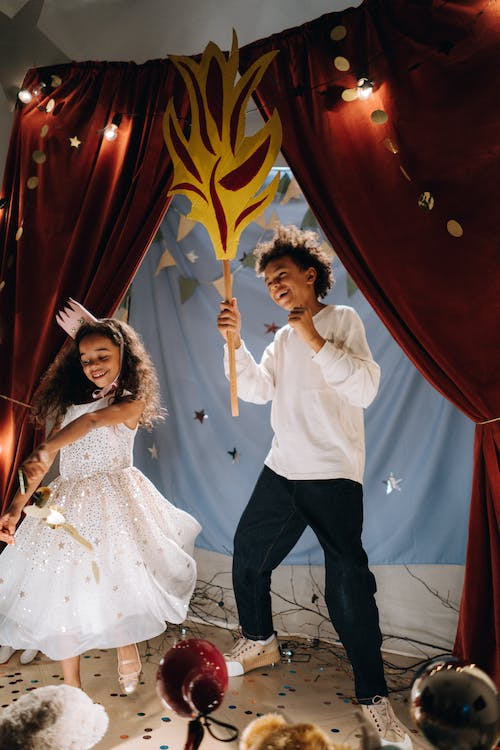
\includegraphics[width=2.43750in,height=3.65625in]{media/image1.jpeg}

\textbf{Textos dramáticos}

Uma história, para ser encenada no teatro, deve ser transformada em
\textbf{roteiro}, isto é, em um texto com uma estrutura adequada para
ser utilizada pelos atores na hora da encenação, sob a orientação de um
diretor.

No roteiro de texto teatral, também chamado de \textbf{texto dramático},
estão descritos os diálogos dos personagens e as rubricas, que consistem
nas orientações acerca da montagem da cena, do figurino e de todas as
situações que necessariamente devem ocorrer no decorrer da peça.

Em textos dramáticos, o enredo é transmitido por meio das ações e dos
diálogos dos personagens, que, nas encenações, são representados por
atores. A representação dos personagens e de suas ações em peças
teatrais e filmes, inseridos em diferentes cenários, espaços e tempo,
torna possível o imaginado ficar mais próximo de quem o representa e do
público que prestigia a atuação.~

Normalmente, um roteiro de texto dramático apresenta os seguintes
elementos: título, lista de personagens, organização do cenário,
rubricas.

\textbf{\textless{}fim do boxe de conteúdo\textgreater{}}

\subsection{Atividades}\label{atividades-1}

Leia o trecho da peça teatral para responder às questões propostas.

Realize uma leitura compartilhada do texto. Chame a atenção dos alunos
para as rubricas no texto e para sua função de orientar a dramatização
(como indicações das formas de falar, caminhar, gesticular; indicação de
características como altura da voz, ritmo). Solicite aos alunos que
observem quem são os personagens e qual é o papel de cada um.

Inserir imagem ao lado do texto:
https://pixabay.com/pt/vectors/violino-violinista-banda-bandsman-154220/

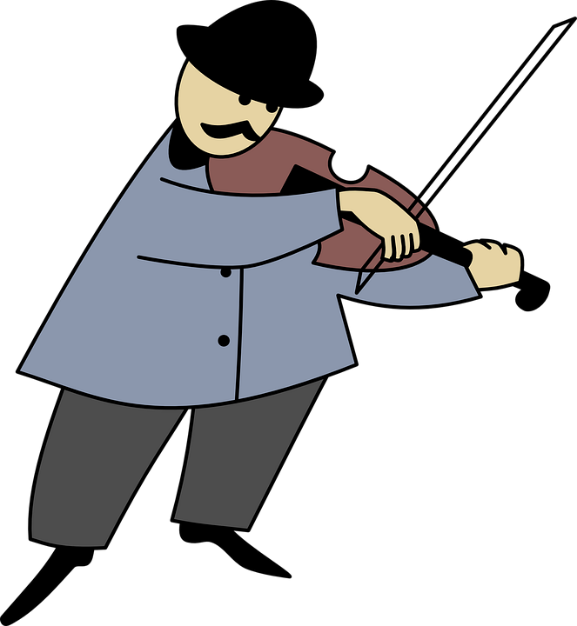
\includegraphics[width=2.61389in,height=2.83858in]{media/image2.png}

\textbf{\textless{}início de texto citado\textgreater{}}

\textbf{Zé Betovi e Nhô Mozarte}

\emph{\emph{Entra Nhô Mozarte com seu livro embaixo do braço olhando em
sua volta e fala em voz alta: }}

\emph{Nhô Mozarte:} Aqui está bem mais tranquilo. Pelo menos não tem
nenhuma obra por perto. Com aquele barulho danado das máquinas eu não
estava conseguindo me concentrar.

(\emph{Em seguida, senta-se no banco da praça e começa a ler.})

\emph{Zé Betovi:} Tchau, mãe! Tô indo lá na praça tocar um pouco.

\protect\hypertarget{_Hlk35856697}{}{}(\emph{Zé Betovi caminha em
direção à praça com seu violino na mão e resolve se sentar perto de uma
árvore, pois o calor estava muito grande naquele dia. Nem notou a
presença de Nhô Mozarte sentado no banco, entretido lendo seu livro, e
começa a tocar. Quando Nhô Mozarte escuta a música, para de ler e
procura ver de onde vem aquele som. Avista Zé Betovi sentado tocando.
Então se levanta devagar, procurando não fazer barulho, e vai em direção
a ele}. \emph{Quando Zé Betovi acaba de tocar, aplaude com entusiasmo.)}

\emph{Nhô Mozarte:} Bravo, meu jovem! Que maravilha! Estou admirado de
ver um garoto de sua idade tocando violino. E um instrumento que não é
fácil. Os jovens assim como você, principalmente nos dias de hoje,
preferem as guitarras, baterias, violão.

\emph{Zé Betovi:} Obrigado. É mesmo... Eu também gosto dos outros
instrumentos. Tenho violão e teclado e toco de vez em quando, mas o meu
preferido mesmo é esse aqui (\emph{mostra o violino.}).

\emph{Nhô Mozarte:} Um artista completo! (\emph{Admiração.}) Então, se
você toca violino, é porque aprecia a música clássica.

\emph{Zé Betovi:} Gosto. E nem tinha como eu não gostar. Lá em casa
tanto meu pai como minha mãe adoram. Na verdade, eu cresci ouvindo. Meu
avô, o pai de minha mãe, tocava muito bem de ouvido e nem sabia ler
partitura.

\emph{Nhô Mozarte:} E você? Toca de ouvido como seu avô?

\emph{Zé Betovi:} Das duas formas. Minha mãe me colocou em aulas de
música desde que eu era bem pequeno. Ela achou que ia ser bom pra mim.
E, quando eu fiz seis anos, escolhi o violino.

\emph{Nhô Mozarte:} Sua mãe fez muito bem. A música é importante na vida
de todo mundo. Ela nos ajuda em tantas coisas... Mas me diga, meu rapaz:
você sabe quem é o autor da música que estava tocando há pouco?

\emph{Zé Betovi:} Villa Lobos

{[}...{]}

Marluzi Moreira de Carvalho. Teatro na escola. Zé Betovi e Nhô Mozarte.
Disponível em:
www.teatronaescola.com/index.php/banco-de-pecas/category/infantil-ou-infanto-juvenil-2.
Acesso em: 15 fev. 2023. Adaptado.

\textbf{\textless{}fim de texto citado\textgreater{}}

\subsubsection{1. }\label{section-16}

Quem são os personagens desse texto? Zé Betovi e Nhô Mozarte.

\_\_\_\_\_\_\_\_\_\_\_\_\_\_\_\_\_\_\_\_\_\_\_\_\_\_\_\_\_\_\_\_\_\_\_\_\_\_\_\_\_\_\_\_\_\_\_\_\_\_\_\_\_\_\_\_\_\_\_\_\_\_\_\_\_\_\_\_\_\_\_\_\_\_\_\_\_\_\_\_\_\_\_\_\_\_\_\_\_\_\_\_\_\_\_\_\_\_\_\_\_\_\_\_\_\_\_\_\_\_\_\_\_\_\_\_\_\_\_\_\_\_\_\_\_\_\_\_\_\_\_\_\_\_\_\_\_\_\_\_

\subsubsection{2. }\label{section-17}

As rubricas no texto servem para orientar a dramatização. Sublinhe cada
uma delas.

\subsubsection{3. }\label{section-18}

Qual é o instrumento preferido de Zé Betovi? O violino.

\protect\hypertarget{_Hlk127362551}{}{}\_\_\_\_\_\_\_\_\_\_\_\_\_\_\_\_\_\_\_\_\_\_\_\_\_\_\_\_\_\_\_\_\_\_\_\_\_\_\_\_\_\_\_\_\_\_\_\_\_\_\_\_\_\_\_\_\_\_\_\_\_\_\_\_\_\_\_\_\_\_\_\_\_\_\_\_\_\_\_\_\_\_\_\_\_\_\_\_\_\_\_\_\_\_\_\_\_\_\_\_\_\_\_\_\_\_\_\_\_\_\_\_\_\_\_\_\_\_\_\_\_\_\_\_\_\_\_\_\_\_\_\_\_\_\_\_\_\_\_\_

\subsubsection{4. }\label{section-19}

Os nomes dos personagens foram inspirados em dois músicos famosos. Você
consegue identificar quem são eles? Mozart e Beethoven.

\_\_\_\_\_\_\_\_\_\_\_\_\_\_\_\_\_\_\_\_\_\_\_\_\_\_\_\_\_\_\_\_\_\_\_\_\_\_\_\_\_\_\_\_\_\_\_\_\_\_\_\_\_\_\_\_\_\_\_\_\_\_\_\_\_\_\_\_\_\_

\subsubsection{5. }\label{section-20}

O texto apresentado é teatral. Com qual objetivo esses textos são
escritos? O objetivo de se escrever textos desse tipo é que sejam
encenados.

\_\_\_\_\_\_\_\_\_\_\_\_\_\_\_\_\_\_\_\_\_\_\_\_\_\_\_\_\_\_\_\_\_\_\_\_\_\_\_\_\_\_\_\_\_\_\_\_\_\_\_\_\_\_\_\_\_\_\_\_\_\_\_\_\_\_\_\_\_\_\_\_\_\_\_\_\_\_\_\_\_\_\_\_\_\_\_\_\_\_\_\_\_\_\_\_\_\_\_\_\_\_\_\_\_\_\_\_\_\_\_\_\_\_\_\_\_\_\_\_\_\_\_\_\_\_\_\_\_\_\_\_\_\_\_\_\_\_\_\_

\subsubsection{6. }\label{section-21}

Releia o trecho a seguir.

\textbf{\textless{}início de texto citado\textgreater{}}

\emph{Nhô Mozarte:} Bravo, meu jovem! Que maravilha! Estou admirado de
ver um garoto de sua idade tocando violino. {[}...{]} Os jovens assim
como você, principalmente nos dias de hoje, preferem as
\textbf{guitarras}, \textbf{baterias}, \textbf{violão}.

\textbf{\textless{}fim de texto citado\textgreater{}}

No espaço a seguir, faça um desenho de cada instrumento musical
destacado e escreva o nome de cada um deles abaixo do desenho.

\textless{}Criar espaço para desenho dos alunos.\textgreater{}

\subsubsection{7. }\label{section-22}

No conto ``João e Maria'', narra-se a história de dois irmãos que são
abandonados pelo pai e pela madrasta na floresta. Leia um trecho desse
conto.

Inserir imagem de floresta:
https://unsplash.com/pt-br/fotografias/6YHlHIVROzg

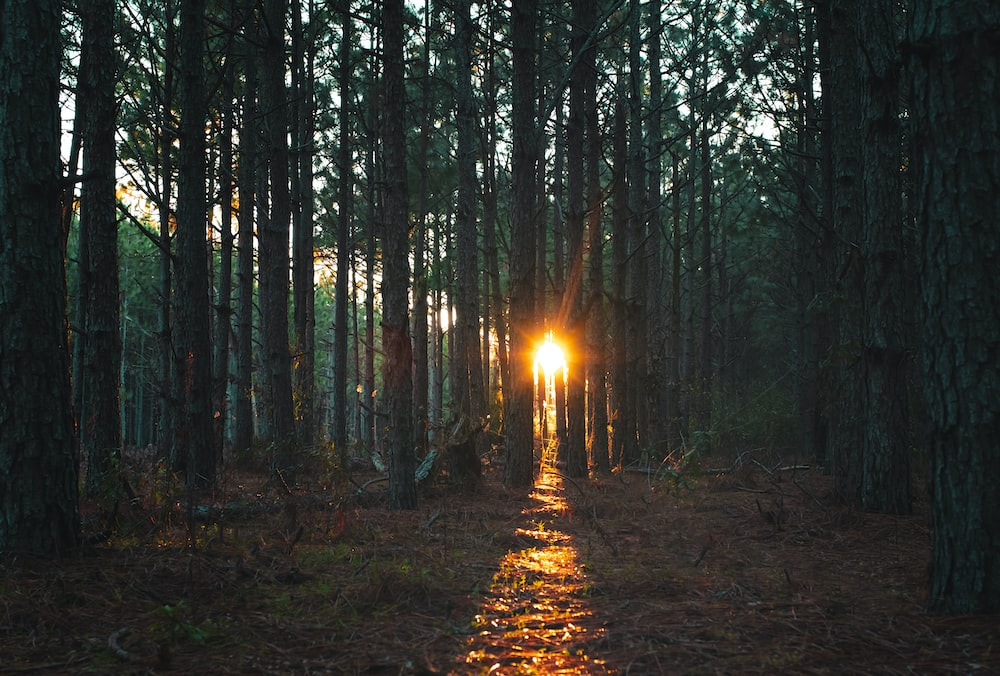
\includegraphics[width=4.08333in,height=2.76048in]{media/image3.jpeg}

\textbf{\textless{}início de texto citado\textgreater{}}

\textbf{João e Maria}

Às margens de uma extensa mata, existia, há muito tempo, uma cabana
pobre, feita de

troncos de árvore, na qual morava um lenhador com sua segunda esposa e
seus dois

filhinhos, nascidos do primeiro casamento. O garoto chamava-se João e a
menina, Maria.

A vida sempre fora difícil na casa do lenhador, mas naquela época as
coisas haviam piorado ainda mais: não havia pão para todos.

\emph{--- Minha mulher, o que será de nós? Acabaremos todos por morrer
de necessidade. E as}

\emph{crianças serão as primeiras\ldots{}}

\emph{--- Há uma solução\ldots{} --- disse a madrasta, que era muito
malvada. --- Amanhã, daremos a João e Maria um pedaço de pão, depois os
levaremos à mata e lá os abandonaremos.}

{[}...{]}

Irmãos Grimm. João e Maria. Disponível em:

www.dominiopublico.gov.br/download/texto/me000589.pdf. Acesso em: 15
fev. 2023.

a) Quem são os personagens dessa história?

João, Maria, o pai e a madrasta.

\_\_\_\_\_\_\_\_\_\_\_\_\_\_\_\_\_\_\_\_\_\_\_\_\_\_\_\_\_\_\_\_\_\_\_\_\_\_\_\_\_\_\_\_\_\_\_\_\_\_\_\_\_\_\_\_\_\_\_\_\_\_\_\_\_\_\_\_\_\_\_\_\_\_\_\_\_\_\_\_\_\_\_\_\_\_\_\_\_\_\_\_\_\_\_\_\_\_\_\_\_\_\_\_\_\_\_\_\_\_\_\_\_\_\_\_\_\_\_\_\_\_\_\_\_\_\_\_\_\_\_\_\_\_\_\_\_\_\_\_

b) Por que a madrasta sugeriu abandonar João e Maria?

A madrasta deu essa sugestão, porque não havia comida para todos.

\_\_\_\_\_\_\_\_\_\_\_\_\_\_\_\_\_\_\_\_\_\_\_\_\_\_\_\_\_\_\_\_\_\_\_\_\_\_\_\_\_\_\_\_\_\_\_\_\_\_\_\_\_\_\_\_\_\_\_\_\_\_\_\_\_\_\_\_\_\_\_\_\_\_\_\_\_\_\_\_\_\_\_\_\_\_\_\_\_\_\_\_\_\_\_\_\_\_\_\_\_\_\_\_\_\_\_\_\_\_\_\_\_\_\_\_\_\_\_\_\_\_\_\_\_\_\_\_\_\_\_\_\_\_\_\_\_\_\_\_

c) Onde eles planejavam abandonar as crianças?

Eles planejavam abandonar as crianças na mata.

\_\_\_\_\_\_\_\_\_\_\_\_\_\_\_\_\_\_\_\_\_\_\_\_\_\_\_\_\_\_\_\_\_\_\_\_\_\_\_\_\_\_\_\_\_\_\_\_\_\_\_\_\_\_\_\_\_\_\_\_\_\_\_\_\_\_\_\_\_\_\_\_\_\_\_\_\_\_\_\_\_\_\_\_\_\_\_\_\_\_\_\_\_\_\_\_\_\_\_\_\_\_\_\_\_\_\_\_\_\_\_\_\_\_\_\_\_\_\_\_\_\_\_\_\_\_\_\_\_\_\_\_\_\_\_\_\_\_\_\_

d) Marque a alternativa correta em relação ao que mostra o trecho
selecionado do conto ``João e Maria''.

( ) A situação de tristeza que tomou conta do pai e da madrasta depois
de eles abandonarem as crianças.

( x ) Os motivos que levaram o pai e a madrasta a pensarem em deixar as
crianças na floresta.

\subsubsection{8. }\label{section-23}

Releia a história e sublinhe no texto:

a) de vermelho, a fala do pai.

b) de verde, a fala da madrasta.

\subsubsection{9. }\label{section-24}

Narrador é aquele que conta a história. Assinale a frase abaixo que
pertence ao narrador.

( x ) O garoto chamava-se João e a menina, Maria.

( ) Minha mulher, o que será de nós?

\subsubsection{10. }\label{section-25}

Releia o trecho a seguir.

\textbf{\textless{}início de texto citado\textgreater{}}

--- Há uma solução\ldots{} --- disse a madrasta, que era muito malvada.
--- Amanhã daremos a João e Maria um pedaço de pão, depois os levaremos
à mata e lá os abandonaremos.

\textbf{\textless{}fim de texto citado\textgreater{}}

Como o leitor sabe quem está falando?

Pelo comentário do narrador depois da fala indicada pelo travessão.

\_\_\_\_\_\_\_\_\_\_\_\_\_\_\_\_\_\_\_\_\_\_\_\_\_\_\_\_\_\_\_\_\_\_\_\_\_\_\_\_\_\_\_\_\_\_\_\_\_\_\_\_\_\_\_\_\_\_\_\_\_\_\_\_\_\_\_\_\_\_\_\_\_\_\_\_\_\_\_\_\_\_\_\_\_\_\_\_\_\_\_\_\_\_\_\_\_\_\_\_\_\_\_\_\_\_\_\_\_\_\_\_\_\_\_\_\_\_\_\_\_\_\_\_\_\_\_\_\_\_\_\_\_\_\_\_\_\_\_\_

\subsubsection{11. }\label{section-26}

Quem conta a história de João e Maria? Assinale a alternativa correta.

Explique aos alunos que, em algumas narrativas, pode acontecer de o
narrador não indicar quem fala; a identificação ocorre pela sequência do
discurso e pela apresentação por meio dos verbos de enunciação.

( ) Um narrador que participa da história (narração em primeira pessoa).

( x ) Um narrador que não participa das ações (narração em terceira
pessoa).

\subsubsection{12. }\label{section-27}

Releia o trecho a seguir.

\textbf{\textless{}início de texto citado\textgreater{}}

\emph{---} Amanhã daremos a João e Maria um pedaço de pão, depois os
levaremos à mata e lá os abandonaremos.

\textbf{\textless{}fim de texto citado\textgreater{}}

a) Circule o sinal usado para destacar a fala da madrasta.

b) Qual é o nome desse sinal que você circulou? Travessão

\_\_\_\_\_\_\_\_\_\_\_\_\_\_\_\_\_\_\_\_\_\_\_\_\_\_\_\_\_\_\_\_\_\_\_\_\_\_\_\_\_\_\_\_\_\_\_\_\_\_\_\_\_\_\_\_\_\_\_\_\_\_\_\_\_\_\_

\subsubsection{13. }\label{section-28}

Os verbos de enunciação são verbos que introduzem a fala. Tendo isso em
vista, releia este trecho:

\textbf{\textless{}início de texto citado\textgreater{}}

--- Há uma solução\ldots{} --- disse a madrasta, que era muito malvada.
{[}...{]}

\textbf{\textless{}fim de texto citado\textgreater{}}

Caso julgue pertinente, incentive a observação de como ficaria esta fala
em um discurso

Indireto, para que os alunos percebam os efeitos de sentido produzidos
pelos verbos de enunciação no discurso direto.

Qual palavra indica o que a madrasta fez? A forma verbal ``disse''.

\_\_\_\_\_\_\_\_\_\_\_\_\_\_\_\_\_\_\_\_\_\_\_\_\_\_\_\_\_\_\_\_\_\_\_\_\_\_\_\_\_\_\_\_\_\_\_\_\_\_\_\_\_\_\_\_\_\_\_\_\_\_\_\_\_\_\_

\subsection{Treino}\label{treino-1}

\subsubsection{1. }\label{section-29}

Leia o trecho do texto, atentando-se às falas dos personagens.

\textbf{\textless{}início de texto citado\textgreater{}}

\textbf{A cabra cabriola }

\textbf{Cena 1} (Maria brinca no pátio e a mãe entra.)

\emph{Mãe}: Maria, minha filhinha, agora vou trabalhar! Você vai ficar
quietinha. Não saia a passear, pois a cabra cabriola anda por este
lugar!

(Maria nem escuta, continua brincando.)

\emph{Mãe}: Maria, sua teimosa! Faça o favor de escutar: se você for
sequestrada, se a cabra a pegar, não tenho dinheiro e joias para o
resgate pagar!

\emph{Maria}: Ah, mamãe, não acredito nessa história. É inventada! Mas
pode ir. Aqui fico neste batente, sentada. {[}...{]}

(A mãe sai e Maria vai passear.)

\emph{Maria:} Obedecer? Ah, quem disse? Vou sair a passear, caçar
borboletas, ninhos, correr, pular e brincar, até pegar passarinhos para
em gaiolas criar!

{[}...{]}

Lourdes Ramalho. Teatro na escola. A cabra cabriola\emph{.} Disponível
em:
www.teatronaescola.com/index.php/banco-de-pecas/category/lourdes-ramalho.
Acesso em: 09 fev. 2023. Adaptado.

\textbf{\textless{}fim de texto citado\textgreater{}}

O texto apresentado é

(A) uma lenda.

(B) uma poesia.

(C) um texto teatral.

(D) uma fábula.

Saeb: D6 - Relacionar, em um texto, assunto e finalidade com o tipo de
texto.

BNCC: EF35LP24: Identificar funções do texto dramático (escrito para ser
encenado) e sua organização por meio de diálogos entre personagens e
marcadores das falas das personagens e de cena.

(A) Incorreta. O texto não explica acontecimentos misteriosos ou
sobrenaturais.

(B) Incorreta. O texto não está organizado em versos.

(C) Correta. O texto apresenta estrutura do texto teatral, marcada pela
descrição dos movimentos de cena (texto secundário indicado entre
parênteses) e pela organização do texto principal em falas.

(D) Incorreta. Nas fábulas, não há descrição de movimentações de cena.

\subsubsection{2. }\label{section-30}

Leia um trecho de texto teatral inspirado em uma fábula de Esopo.

\textbf{\textless{}início de texto citado\textgreater{}}

\textbf{A toupeira avarenta}

Personagens: toupeira, tatu, avestruz.

Cenário: um campo.

(Toupeira está cavando um buraco. É observada, de longe, por um tatu.)

\emph{Toupeira:} Meu tesouro, cadê você, meu tesouro?

\emph{Tatu:} (à parte) Ora, ora, ora...

\emph{Toupeira:} (falando a uma barra de ouro que acaba de tirar do
buraco) Ah, aí está você: tudo o que tenho é esta bela barra de ouro.

\emph{Tatu:} (à parte) Ora, ora, ora...

\emph{Toupeira:} (enterrando novamente a barra de ouro) Bem, já chega.
Amanhã eu volto pra ver você de novo...

{[}...{]}

José Carlos Aragão. \emph{No palco, todo mundo vira bicho:} novas
fábulas de Esopo adaptadas para teatro. São Paulo: Planeta do Brasil,
2007. p. 39.

\textbf{\textless{}fim de texto citado\textgreater{}}

As peças teatrais são criadas para serem usadas em encenações por atores
em teatros. Essas peças são semelhantes:

(A) ao roteiro de cinema.

(B) à entrevista.

(C) à reportagem.

(D) ao jornal de rádio.

Saeb: D10 - Diferenciar, por comparação ou identificação de
características, textos de diferentes gêneros (notícia x narrativa
ficcional; notícia x texto expositivo de outras áreas;

propaganda x anúncio).

BNCC: EF35LP24 - Identificar funções do texto dramático (escrito para
ser encenado) e sua organização por meio de diálogos entre personagens e
marcadores das falas das personagens e de cena.

.

(A) Correta. Roteiros cinematográficos, assim como as peças teatrais,
são elaborados para serem encenados por atores em filmes.

(B) Incorreta. Entrevista consiste em gênero informativo que apresenta
entrevistador e entrevistado.

(C) Incorreta. Reportagens são textos informativos veiculados por
diversos meios de comunicação e têm como conteúdo informações reais e
atuais.

(D) Incorreta. Jornal de rádio transmite as notícias da atualidade por
meio de emissões radiofônicas.

\subsubsection{3. }\label{section-31}

Leia o trecho do conto ``Água da vida''.

\textbf{\textless{}início de texto citado\textgreater{}}

\textbf{Água da vida}

Houve, uma vez, um rei muito poderoso, que vivia feliz e tranquilo em
seu reino. Um belo dia, adoeceu gravemente e ninguém tinha esperanças de
que escapasse. Ele tinha três filhos, {[}...{]}.

Encontravam-se eles no jardim do castelo a chorar e, de repente, viram
surgir à sua frente um velho de aspecto venerável, que indagou a causa
de tamanha tristeza. Disseram-lhe que estavam aflitos porque o pai
estava gravemente enfermo e os médicos já não tinham esperanças de o
salvar.

O velho, então, disse-lhe:

- Eu conheço um remédio muito eficaz, que poderá curá-lo; é a famosa
Água da Vida. Mas é muito difícil obtê-la.

{[}...{]}

\textbf{\textless{}fim de texto citado\textgreater{}}

Irmãos Grimm. A água da vida. Disponível em:
https://www.grimmstories.com/pt/grimm\_contos/a\_agua\_da\_vida. Acesso
em: 16 fev. 2023.

Em relação ao narrador do conto, ele

(A) participa da história.

(B) não participa da história.

(C) é personagem da história.

(D) realiza ações da história.

Saeb: D7: Relacionar, na compreensão do texto, informações textuais com
conhecimentos de senso comum.

BNCC: EF35LP26 - Ler e compreender, com certa autonomia, narrativas
ficcionais que apresentem cenários e personagens, observando os
elementos da estrutura narrativa: enredo, tempo, espaço, personagens,
narrador e a construção do discurso indireto e discurso direto.

.(A) Incorreta. Não existe ``eu'' ou ``nós'' no conto para se afirmar
que o narrador participe da história.

(B) Correta. O narrador não realiza as ações da história, mas narra os
acontecimentos.

(C) Incorreta. O narrador não é um personagem da história.

(D) Incorreta. O narrador não pratica nenhuma ação narrada.

\section{Módulo 3}\label{muxf3dulo-3}

Neste módulo, espera-se que os alunos identifiquem os sinais de
pontuação e analisem os efeitos de sentido decorrentes do uso da
pontuação em diversos tipos de textos. Habilidades da BNCC: EF03LP07 e
EF03LP16.

\textbf{Habilidades SAEB}

- Analisar elementos constitutivos de gêneros textuais diversos.

- Reconhecer os usos da pontuação.

- Analisar os efeitos de sentido decorrentes do uso da pontuação.

\subsection{Conteúdo}\label{conteuxfado-2}

\textbf{\textless{}início do boxe de conteúdo\textgreater{}}

\textbf{Pontuação}

\textbf{https://pixabay.com/pt/illustrations/sinais-de-pontua\%c3\%a7\%c3\%a3o-palavra-l\%c3\%adngua-2999583/}

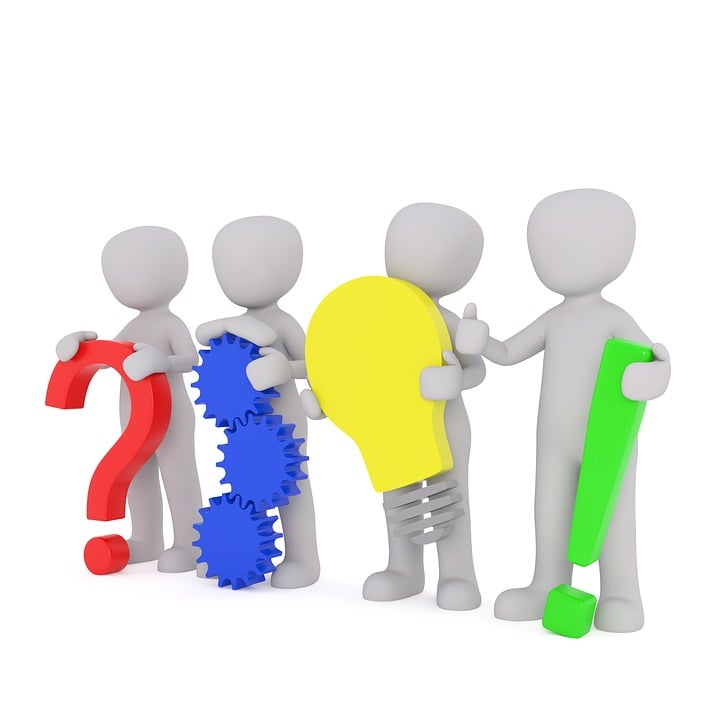
\includegraphics[width=3.41667in,height=3.41667in]{media/image4.jpeg}

Os sinais de pontuação têm variadas funções em um texto escrito e ajudam
bastante a compreender a construção de sentidos pretendida por quem
escreve um texto. Para entender melhor, leia um trecho do conto ``O
rouxinol do imperador'', atentando-se à pontuação.

\textbf{\textless{}início de texto citado\textgreater{}}

\textbf{O rouxinol do imperador}

{[}...{]}

Um dia, um {[}livro{]} chegou às mãos do imperador. O soberano o leu e
ficou, ao mesmo tempo, surpreso e enfurecido. Mandou logo chamar o
primeiro-ministro.

--- Incrível! No bosque que faz divisa com os jardins imperiais, vive um
rouxinol cujo canto é incomparável, e eu o desconheço! Tive que ler um
livro estrangeiro para aprender que a maior maravilha de meu país é um
pássaro de voz de ouro, e não este meu soberbo palácio! Diga-me, por que
não fui informado?

--- Eu também ignorava o fato, meu senhor --- respondeu o
primeiro-ministro, assustado com a ira do imperador. --- Mas vou
descobri-lo.

--- E que seja muito breve. Nesta noite mesmo o rouxinol deverá cantar
somente para mim.

{[}...{]}

Hans Christian Andersen. O rouxinol do imperador. Disponível em:
\url{http://www.dominiopublico.gov.br/download/texto/me000589.pdf}.
Acesso em: 16 fev. 2023.

\textbf{\textless{}fim de texto citado\textgreater{}}

O texto apresenta vários sinais de pontuação: ponto final (\textbf{.}),
travessão (\textbf{---}), ponto de exclamação (\textbf{!}) e ponto de
interrogação (\textbf{?}). Perceba que o travessão marca a voz das
personagens; e esses diálogos fazem com que o leitor tenha a sensação de
assistir à conversa, como se acontecesse no momento em que lê. O ponto
de exclamação intensifica os sentimentos de indignação. O ponto de
interrogação indica a entonação utilizada ao se fazer pergunta. O ponto
final marca o fim de uma frase.

\textbf{\textless{}fim do boxe de conteúdo\textgreater{}}

\subsection{Atividades}\label{atividades-2}

\subsubsection{1. }\label{section-32}

Leia o texto a seguir. Em seguida, responda às atividades propostas.

Inserir imagem ao lado do texto:
https://pixabay.com/pt/vectors/lobo-bonitinho-animal-personagem-1454420/


\includegraphics[width=1.97917in,height=3.16667in]{media/image5.png}

\textbf{\textless{}início de texto citado\textgreater{}}

\textbf{O lobo e o cordeiro}

Um lobo estava bebendo água num riacho. Um cordeirinho chegou e também
começou a beber, um pouco mais para baixo.

O lobo arreganhou os dentes e disse ao cordeiro:

--- Como é que você tem a ousadia de vir sujar a água que estou bebendo?

--- Como sujar? --- Respondeu o cordeiro. --- A água corre daí para cá,
logo eu não posso estar sujando sua água.

--- Não me responda! --- Tornou o lobo furioso.

--- Há seis meses seu pai me fez a mesma coisa!

--- Há seis meses eu nem tinha nascido. Como é que eu posso ter culpa
disso? --- Respondeu o cordeiro.

--- Mas você estragou todo o meu pasto --- Replicou o lobo.

--- Como é que posso ter estragado seu pasto, se nem dentes eu tenho?

O lobo, não tendo mais como culpar o cordeiro, não disse mais nada:
pulou sobre ele e o devorou.

O LOBO e o cordeiro. Disponível em:
\url{http://www.dominiopublico.gov.br/download/texto/me000589.pdf}.
Acesso em: 16 fev. 2023.

\textbf{\textless{}fim de texto citado\textgreater{}}

a) Quem são os personagens do texto? O lobo e o cordeiro.

\_\_\_\_\_\_\_\_\_\_\_\_\_\_\_\_\_\_\_\_\_\_\_\_\_\_\_\_\_\_\_\_\_\_\_\_\_\_\_\_\_\_\_\_\_\_\_\_\_\_\_\_\_\_\_\_\_\_\_\_\_\_\_\_\_\_\_\_\_\_\_\_\_\_\_\_\_\_\_\_\_\_\_\_\_\_\_\_\_\_\_\_\_\_\_\_\_\_\_\_\_\_\_\_\_\_\_\_\_\_\_\_\_\_\_\_\_\_\_\_\_\_\_\_\_\_\_\_\_\_\_\_\_\_\_\_\_\_\_\_

b) Onde a história acontece? Provavelmente, na floresta, em um riacho.

\_\_\_\_\_\_\_\_\_\_\_\_\_\_\_\_\_\_\_\_\_\_\_\_\_\_\_\_\_\_\_\_\_\_\_\_\_\_\_\_\_\_\_\_\_\_\_\_\_\_\_\_\_\_\_\_\_\_\_\_\_\_\_\_\_\_\_\_\_\_\_\_\_\_\_\_\_\_\_\_\_\_\_\_\_\_\_\_\_\_\_\_\_\_\_\_\_\_\_\_\_\_\_\_\_\_\_\_\_\_\_\_\_\_\_\_\_\_\_\_\_\_\_\_\_\_\_\_\_\_\_\_\_\_\_\_\_\_\_\_

c) Qual é o assunto tratado no texto? Trata-se da história de um lobo
que queria encontrar motivos para matar o cordeiro.

\_\_\_\_\_\_\_\_\_\_\_\_\_\_\_\_\_\_\_\_\_\_\_\_\_\_\_\_\_\_\_\_\_\_\_\_\_\_\_\_\_\_\_\_\_\_\_\_\_\_\_\_\_\_\_\_\_\_\_\_\_\_\_\_\_\_\_\_\_\_\_\_\_\_\_\_\_\_\_\_\_\_\_\_\_\_\_\_\_\_\_\_\_\_\_\_\_\_\_\_\_\_\_\_\_\_\_\_\_\_\_\_\_\_\_\_\_\_\_\_\_\_\_\_\_\_\_\_\_\_\_\_\_\_\_\_\_\_\_\_

\_\_\_\_\_\_\_\_\_\_\_\_\_\_\_\_\_\_\_\_\_\_\_\_\_\_\_\_\_\_\_\_\_\_\_\_\_\_\_\_\_\_\_\_\_\_\_\_\_\_\_\_\_\_\_\_\_\_\_\_\_\_\_\_\_\_\_\_\_\_

\subsubsection{2. }\label{section-33}

Releia este trecho do texto.

\textbf{\textless{}início de texto citado\textgreater{}}

--- Não me responda! --- tornou o lobo furioso.

--- Há seis meses seu pai me fez a mesma coisa! --- Há seis meses eu nem
tinha nascido, como é que eu posso ter culpa disso? --- respondeu o
cordeiro.

\textbf{\textless{}fim de texto citado\textgreater{}}

a) Que sinal de pontuação aparece no fim de cada frase? Ponto final,
ponto de exclamação e ponto de interrogação.

\protect\hypertarget{_Hlk127460239}{}{}\_\_\_\_\_\_\_\_\_\_\_\_\_\_\_\_\_\_\_\_\_\_\_\_\_\_\_\_\_\_\_\_\_\_\_\_\_\_\_\_\_\_\_\_\_\_\_\_\_\_\_\_\_\_\_\_\_\_\_\_\_\_\_\_\_\_\_\_\_\_\_\_\_\_\_\_\_\_\_\_\_\_\_\_\_\_\_\_\_\_\_\_\_\_\_\_\_\_\_\_\_\_\_\_\_\_\_\_\_\_\_\_\_\_\_\_\_\_\_\_\_\_\_\_\_\_\_\_\_\_\_\_\_\_\_\_\_\_\_\_

\_\_\_\_\_\_\_\_\_\_\_\_\_\_\_\_\_\_\_\_\_\_\_\_\_\_\_\_\_\_\_\_\_\_\_\_\_\_\_\_\_\_\_\_\_\_\_\_\_\_\_\_\_\_\_\_\_\_\_\_\_\_\_\_\_\_\_\_\_\_

b) Explique a função de cada um desses sinais de pontuação. Usa-se o
ponto final quando se quer finalizar uma frase ou um período. Utiliza-se
o ponto de exclamação para enfatizar o que foi dito. Usa-se o ponto de
interrogação quando se formula uma pergunta.

Explique aos alunos que frases terminadas com ponto final denominam-se
\textbf{frases declarativas}; as terminadas com ponto de interrogação
denominam-se \textbf{frases interrogativas}; as que terminam com ponto
de exclamação denominam-se \textbf{frases exclamativas}.

\_\_\_\_\_\_\_\_\_\_\_\_\_\_\_\_\_\_\_\_\_\_\_\_\_\_\_\_\_\_\_\_\_\_\_\_\_\_\_\_\_\_\_\_\_\_\_\_\_\_\_\_\_\_\_\_\_\_\_\_\_\_\_\_\_\_\_\_\_\_\_\_\_\_\_\_\_\_\_\_\_\_\_\_\_\_\_\_\_\_\_\_\_\_\_\_\_\_\_\_\_\_\_\_\_\_\_\_\_\_\_\_\_\_\_\_\_\_\_\_\_\_\_\_\_\_\_\_\_\_\_\_\_\_\_\_\_\_\_\_

\_\_\_\_\_\_\_\_\_\_\_\_\_\_\_\_\_\_\_\_\_\_\_\_\_\_\_\_\_\_\_\_\_\_\_\_\_\_\_\_\_\_\_\_\_\_\_\_\_\_\_\_\_\_\_\_\_\_\_\_\_\_\_\_\_\_\_\_\_\_

\_\_\_\_\_\_\_\_\_\_\_\_\_\_\_\_\_\_\_\_\_\_\_\_\_\_\_\_\_\_\_\_\_\_\_\_\_\_\_\_\_\_\_\_\_\_\_\_\_\_\_\_\_\_\_\_\_\_\_\_\_\_\_\_\_\_\_\_\_\_

c) O segundo travessão que ocorre em cada caso tem que função?

A segunda ocorrência do travessão marca o fim da fala do personagem e o
início da intervenção do narrador.

\begin{quote}
\_\_\_\_\_\_\_\_\_\_\_\_\_\_\_\_\_\_\_\_\_\_\_\_\_\_\_\_\_\_\_\_\_\_\_\_\_\_\_\_\_\_\_\_\_\_\_\_\_\_\_\_\_\_\_\_\_\_\_\_\_\_\_\_\_\_\_

\_\_\_\_\_\_\_\_\_\_\_\_\_\_\_\_\_\_\_\_\_\_\_\_\_\_\_\_\_\_\_\_\_\_\_\_\_\_\_\_\_\_\_\_\_\_\_\_\_\_\_\_\_\_\_\_\_\_\_\_\_\_\_\_\_\_\_

\_\_\_\_\_\_\_\_\_\_\_\_\_\_\_\_\_\_\_\_\_\_\_\_\_\_\_\_\_\_\_\_\_\_\_\_\_\_\_\_\_\_\_\_\_\_\_\_\_\_\_\_\_\_\_\_\_\_\_\_\_\_\_\_\_\_\_
\end{quote}

\subsubsection{3. }\label{section-34}

Releia o fim da história:

\textbf{\textless{}início de texto citado\textgreater{}}

O lobo, não tendo mais como culpar o cordeiro, não disse mais nada:
pulou sobre ele e o devorou.

\textbf{\textless{}fim de texto citado\textgreater{}}

\begin{itemize}
\item
  O que essa frase expressa? Marque a alternativa correta.
\end{itemize}

\begin{quote}
( ) Dúvida.

( ) Surpresa.

( x ) Afirmação.
\end{quote}

\subsubsection{4. }\label{section-35}

Leia o trecho de um conto tradicional.

\textbf{\textless{}Arte: colocar cor nos sinais destacados com
grifa-texto.\textgreater{}}

Inserir imagem ao lado do texto:
https://www.istockphoto.com/br/vetor/branca-de-neve-ilustra\%C3\%A7\%C3\%A3o-vetorial-gm521993146-91504715?utm\_source=pixabay\&utm\_medium=affiliate\&utm\_campaign=SRP\_illustration\_sponsored\&utm\_content=https\%3A\%2F\%2Fpixabay.com\%2Fpt\%2Fillustrations\%2Fsearch\%2Fbranca\%2520de\%2520neve\%2F\&utm\_term=branca+de+neve

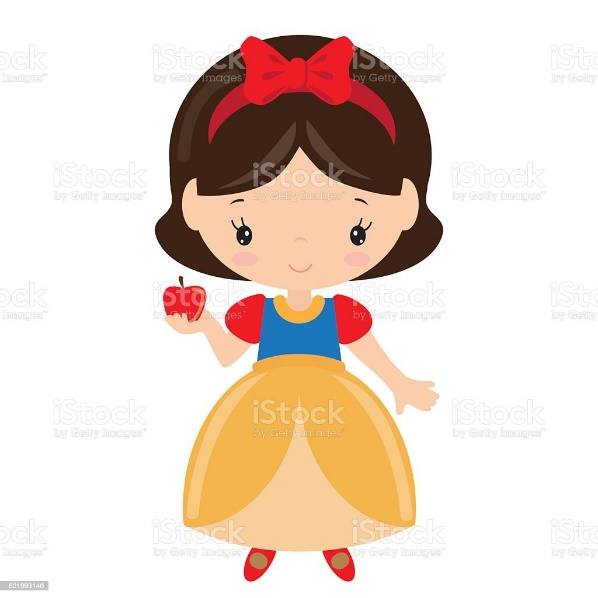
\includegraphics[width=2.71875in,height=2.71875in]{media/image6.jpeg}

\begin{quote}
\textbf{\textless{}início de texto citado\textgreater{}}

\textbf{Branca de Neve}

{[}...{]}

Alguns meses depois, o desejo da rainha foi atendido. Ela deu à luz uma
menina de cabelos bem pretos, pele branca e face rosada. O nome dado à
princesinha foi Branca de Neve.

Mas, quando nasceu a menina, a rainha morreu. Passado um ano, o rei se
casou novamente. Sua esposa era lindíssima, mas muito vaidosa, invejosa
e cruel.

Um feiticeiro lhe dera um espelho mágico, ao qual todos os dias ela
perguntava, com vaidade:

--- Espelho, espelho meu, diga-me se há no mundo mulher mais bela do que
eu.

E o espelho respondia:

--- Em todo o mundo, minha querida rainha, não existe beleza maior.

{[}...{]}

BRANCA de Neve. Disponível em:
http://www.dominiopublico.gov.br/download/texto/me000589.pdf. Acesso em:
16 fev. 2023.

\textbf{\textless{}fim de texto citado\textgreater{}}
\end{quote}

\begin{enumerate}
\def\labelenumi{\alph{enumi})}
\item
  O que a esposa do rei perguntava todos os dias ao espelho? Ela
  perguntava se no mundo havia mulher mais bela do que ela.
\end{enumerate}

\_\_\_\_\_\_\_\_\_\_\_\_\_\_\_\_\_\_\_\_\_\_\_\_\_\_\_\_\_\_\_\_\_\_\_\_\_\_\_\_\_\_\_\_\_\_\_\_\_\_\_\_\_\_\_\_\_\_\_\_\_\_\_\_

\_\_\_\_\_\_\_\_\_\_\_\_\_\_\_\_\_\_\_\_\_\_\_\_\_\_\_\_\_\_\_\_\_\_\_\_\_\_\_\_\_\_\_\_\_\_\_\_\_\_\_\_\_\_\_\_\_\_\_\_\_\_\_\_

\begin{enumerate}
\def\labelenumi{\alph{enumi})}
\item
  Dos sinais de pontuação estão destacados no texto. Qual indica o
  início da fala do personagem? O travessão
\end{enumerate}

\begin{quote}
\protect\hypertarget{_Hlk127463829}{}{}\_\_\_\_\_\_\_\_\_\_\_\_\_\_\_\_\_\_\_\_\_\_\_\_\_\_\_\_\_\_\_\_\_\_\_\_\_\_\_\_\_\_\_\_\_\_\_\_\_\_\_\_\_\_\_\_\_\_\_\_\_\_\_\_\_\_\_

c) Qual sinal anuncia que o personagem vai falar? Os dois-pontos.

\_\_\_\_\_\_\_\_\_\_\_\_\_\_\_\_\_\_\_\_\_\_\_\_\_\_\_\_\_\_\_\_\_\_\_\_\_\_\_\_\_\_\_\_\_\_\_\_\_\_\_\_\_\_\_\_\_\_\_\_\_\_\_\_\_\_\_

d) Se a frase ``--- Espelho, espelho meu, diga-me se há no mundo mulher
mais bela do que eu.'' fosse uma pergunta, como ela seria escrita?
Marque a alternativa correta.
\end{quote}

( x ) --- Espelho, espelho meu, há no mundo mulher mais bela do que eu?

( ) --- Espelho, espelho meu, diga-me se há no mundo mulher mais bela do
que eu!

\subsection{Treino}\label{treino-2}

\subsubsection{1.}\label{section-36}

Leia o anúncio da campanha de vacinação contra o sarampo.

\begin{quote}
https://www.pmna.ms.gov.br/noticias/saude/sarampo-filhos-de-seis-meses-a-menores-de-um-ano-de-idade-que-irao-viajar-para-municipios-em-situacao-de-surto-ativo-devem-vacinar
\end{quote}


\includegraphics[width=4.68681in,height=2.81736in]{media/image7.jpeg}

A frase do anúncio é:

\begin{enumerate}
\def\labelenumi{(\Alph{enumi})}
\item
  declarativa.
\item
  exclamativa.
\item
  interrogativa.
\item
  negativa.
\end{enumerate}

\begin{quote}
Saeb: D16: Analisar efeito de sentido consequente do uso de pontuação
expressiva (interrogação, exclamação, reticências).

BNCC: EF03LP07 - Identificar a função na leitura e usar na escrita ponto
final, ponto de interrogação, ponto de exclamação e, em diálogos
(discurso direto), dois-pontos e travessão.

(A) Incorreta. Frases declarativas terminam com ponto final.

(B) Correta. A frase apresenta ponto de exclamação.

(C) Incorreta. A frase não é uma pergunta.

(D) Incorreta. A frase não expressa negação.
\end{quote}

\subsubsection{2. }\label{section-37}

Leia o trecho a seguir extraído da história \textbf{O gato de botas}.

\begin{quote}
\textbf{\textless{}início de texto citado\textgreater{}}

Um lavrador trabalhara muito, durante a vida toda, ganhando sempre o
suficiente para o sustento da família. Quando faleceu, deixou sua
herança para os filhos: um sítio, um burrinho e um gato.

Ao filho mais velho coube o sítio; ao segundo, o burrinho; e o caçula
ficou com o gato. Este último, nada satisfeito com o que lhe coubera,
resmungou: ``Meus irmãos sobreviverão honestamente. Mas e eu? O que vou
fazer? Talvez possa jantar o gato e com o couro fazer um tamborim. Mas e
depois?''

O gato logo endireitou as orelhas, querendo ouvir melhor um assunto de
tamanho interesse. Então, percebendo que precisava agir, foi dizendo:

--- Não se desespere, patrãozinho, pois eu tenho um plano. Consiga-me um
par de botas e um saco de pano, e deixe o resto comigo.

{[}...{]}

\textbf{\textless{}fim de texto citado\textgreater{}}

O GATO de Botas. Disponível em:
\url{http://www.dominiopublico.gov.br/download/texto/me000589.pdf}.
Acesso em: 17 fev. 2023.

Que sinal de pontuação indica a presença de um diálogo no trecho?
\end{quote}

\begin{enumerate}
\def\labelenumi{(\Alph{enumi})}
\item
  A vírgula.
\item
  O ponto final.
\item
  O travessão.
\item
  O ponto de interrogação.
\end{enumerate}

\protect\hypertarget{_Hlk127521720}{}{}Saeb: D17 - Compreender a
utilização de notações como travessão, aspas, dois pontos e reticências
na construção de um texto.

BNCC: EF03LP07: Identificar a função na leitura e usar na escrita ponto
final, ponto de interrogação, ponto de exclamação e, em diálogos
(discurso direto), dois-pontos e travessão.

.

(A) Incorreta. A vírgula não serve para indicar diálogos, mas para
separar elementos dentro de uma mesma frase.

(B) Incorreta. O ponto final~é um sinal de pontuação que encerra o
período.

(C) Correta. O~travessão~é um sinal de pontuação usado especialmente no
início de cada fala no discurso direto.

(D) Incorreta. O~ponto de interrogação~é usado para indicar uma
pergunta.

\subsubsection{3.}\label{section-38}

Leia o trecho de um manual.

\begin{quote}
\textbf{\textless{}início de texto citado\textgreater{}}

\textbf{Manual Aventura Científica}

{[}...{]}

1- Destaque as cartas.

2- Embaralhe as cartas EU QUERO SABER e deixe-as em um monte com a

face Eu Quero Saber virada para cima, no lugar marcado no tabuleiro.

3- Embaralhe as cartas A-HÁ e deixe-as em um monte, com a face A-HÁ
virada para cima, no lugar marcado no tabuleiro.

4- Deixe as peças dos quadros espalhadas ao lado do tabuleiro, com o
lado da

ilustração virada para cima, ao alcance de todos os jogadores.

5- Cada jogador escolhe um peão e coloca-o no local marcado no
tabuleiro.

{[}...{]}

MANUAL Aventura Científica. Disponível em:
https://estrela.vteximg.com.br/arquivos/Manual-

Aventura-Cientifica-Show-da-Luna.pdf. Acesso em: 17 fev. 2023.

\textbf{\textless{}início de texto citado\textgreater{}}

O objetivo desse texto é

(A) dar informações relacionadas à ciência.

(B) mostrar as instruções relativas a um jogo.

(C) convencer o leitor a jogar um jogo de aventura.

(D) ajudar o leitor a solucionar problemas de um jogo.
\end{quote}

Saeb: D9 - Realizar inferências e antecipações em relação ao conteúdo e
à intencionalidade a partir de indicadores como tipo de texto e
características gráficas.

BNCC EF03LP16 - Identificar e reproduzir, em textos injuntivos
instrucionais (receitas, instruções de montagem, digitais ou impressos),
a formatação própria desses textos (verbos imperativos, indicação de
passos a ser seguidos) e a diagramação específica dos textos desses
gêneros (lista de ingredientes ou materiais e instruções de execução --
"modo de fazer").

(A) Incorreta. O trecho apresenta instruções de um jogo, e não
informações relacionadas à ciência.

(B) Correta. O manual mostra instruções de como jogar o jogo ``Aventura
científica''.

(C) Incorreta. O manual não tem como finalidade convencer o leitor, já
que ele apenas apresenta instruções do jogo.

(D) Incorreta. O texto ajuda o leitor a jogar o jogo, e não a solucionar
problemas.

\section{Módulo 4}\label{muxf3dulo-4}

Orientação para o professor: Neste módulo, espera-se que os alunos leiam
e compreendam autonomamente texto do campo da vida pública; relacionem a
imagem no texto à mensagem (linguagens verbal e não verbal); relacionem
a finalidade do texto às estratégias de convencimento; identifiquem a
função social do texto, reconhecendo para que serve e a quem se destina;
identifiquem a ideia central do texto, compreendendo-o globalmente e
infiram informações implícitas no texto.

\textbf{Habilidades BNCC: EF03LP19}

\textbf{Habilidades SAEB}

\textbf{- Analisar o uso de recursos de persuasão em textos verbais e/ou
multimodais.}

\textbf{- Analisar os efeitos de sentido de recursos multissemióticos em
textos que circulam em diferentes suportes.}

\textbf{- Julgar a eficácia de argumentos em textos.}

\subsection{Conteúdo}\label{conteuxfado-3}

\textbf{Textos publicitários}

\textbf{https://pixabay.com/pt/photos/paris-fran\%c3\%a7a-cidade-cidades-urbano-195327/}

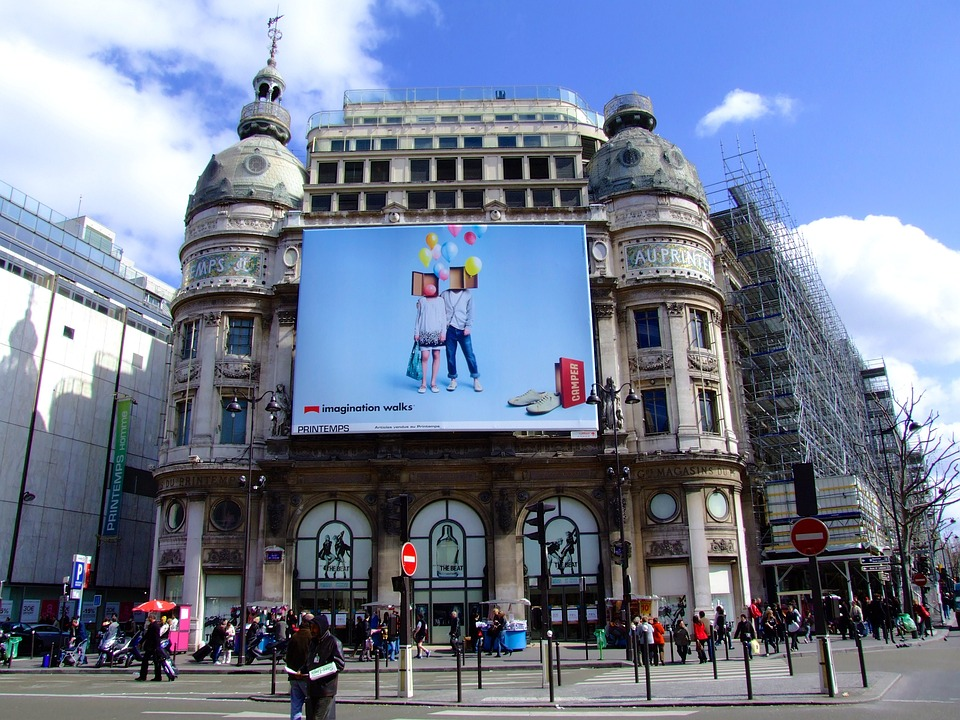
\includegraphics[width=4.83333in,height=3.62500in]{media/image8.jpeg}

Anúncio publicitário ou de propaganda consiste em um gênero textual que
tem como finalidade divulgar uma ideia, um produto, um valor ou um
conceito. Essa divulgação é feita para convencer, isto é, persuadir o
público em relação ao ao que está sendo veiculado, tanto a comprar um
produto, a realizar uma ação como a adotar um comportamento.

Como o principal objetivo do anúncio é persuadir e convencer o leitor,
todos os elementos nele presentes são muito bem pensados. Para atingir
seu objetivo, quem o elabora se utiliza da linguagem verbal (escrita),
da linguagem não verbal (imagens) e de outros artifícios, como
combinação de cores, disposição de elementos visuais, jogo de palavras e
imagens etc.

A linguagem normalmente é objetiva e o vocabulário utilizado é dirigido
ao público ao qual o anúncio se destina.

Os anúncios podem ser constituídos de \emph{slogans} (frases de efeito)
e apresentam também a instituição ou a marca responsável pela sua
veiculação (logomarca).

Esse gênero textual pode ser divulgado na televisão, em revistas,
jornais, \emph{outdoors}, cartazes e anúncios na internet.

\subsection{Atividades}\label{atividades-3}

\subsubsection{1. }\label{section-39}

Leia este anúncio publicitário.

Explore com os alunos o cartaz, a imagem que o compõe e os elementos
verbais. Avalie com eles os motivos da escolha do produtor ao dar ênfase
a alguns elementos do texto verbal, e se esse recurso foi efetivo na
divulgação do que ele pretendia.

https://www.folhavitoria.com.br/geral/blogs/petblog/2011/06/09/cachorro-nao-e-brinquedo/

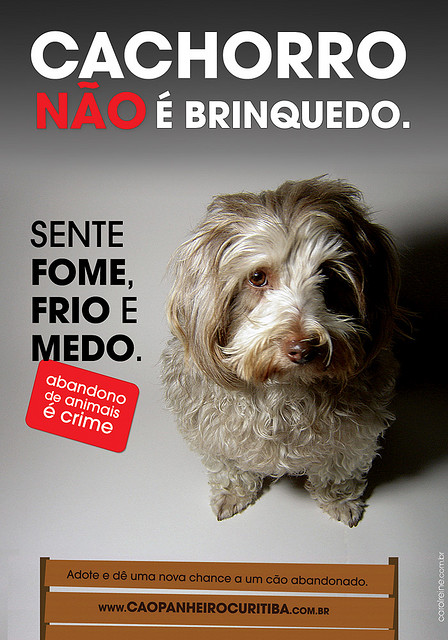
\includegraphics[width=3.11354in,height=4.44792in]{media/image9.jpeg}

a) Qual é o objetivo desse anúncio publicitário?

Espera-se que os alunos compreendam que o objetivo é incentivar as
pessoas a cuidarem dos animais de estimação.

\_\_\_\_\_\_\_\_\_\_\_\_\_\_\_\_\_\_\_\_\_\_\_\_\_\_\_\_\_\_\_\_\_\_\_\_\_\_\_\_\_\_\_\_\_\_\_\_\_\_\_\_\_\_\_\_\_\_\_\_\_\_\_\_

\_\_\_\_\_\_\_\_\_\_\_\_\_\_\_\_\_\_\_\_\_\_\_\_\_\_\_\_\_\_\_\_\_\_\_\_\_\_\_\_\_\_\_\_\_\_\_\_\_\_\_\_\_\_\_\_\_\_\_\_\_\_\_\_

b) Para quem esse anúncio é destinado? É destinado aos donos de animais
de estimação.

\_\_\_\_\_\_\_\_\_\_\_\_\_\_\_\_\_\_\_\_\_\_\_\_\_\_\_\_\_\_\_\_\_\_\_\_\_\_\_\_\_\_\_\_\_\_\_\_\_\_\_\_\_\_\_\_\_\_\_\_\_\_\_\_

\_\_\_\_\_\_\_\_\_\_\_\_\_\_\_\_\_\_\_\_\_\_\_\_\_\_\_\_\_\_\_\_\_\_\_\_\_\_\_\_\_\_\_\_\_\_\_\_\_\_\_\_\_\_\_\_\_\_\_\_\_\_\_\_

c) Segundo o anúncio, por que não devemos abandonar os animais? Porque
eles sentem fome, frio e medo.

\_\_\_\_\_\_\_\_\_\_\_\_\_\_\_\_\_\_\_\_\_\_\_\_\_\_\_\_\_\_\_\_\_\_\_\_\_\_\_\_\_\_\_\_\_\_\_\_\_\_\_\_\_\_\_\_\_\_\_\_\_\_\_\_

\_\_\_\_\_\_\_\_\_\_\_\_\_\_\_\_\_\_\_\_\_\_\_\_\_\_\_\_\_\_\_\_\_\_\_\_\_\_\_\_\_\_\_\_\_\_\_\_\_\_\_\_\_\_\_\_\_\_\_\_\_\_\_\_

d) O cachorro do anúncio aparenta estar:

( ) feliz ( x ) triste ( ) cansado

e) Em sua opinião, na frase ``Cachorro não é brinquedo'', por que a
palavra \textbf{não} está com uma cor diferente do restante do texto?
Resposta pessoal. Para dar destaque ao ato de não abandonar.

\_\_\_\_\_\_\_\_\_\_\_\_\_\_\_\_\_\_\_\_\_\_\_\_\_\_\_\_\_\_\_\_\_\_\_\_\_\_\_\_\_\_\_\_\_\_\_\_\_\_\_\_\_\_\_\_\_\_\_\_\_\_\_\_

\_\_\_\_\_\_\_\_\_\_\_\_\_\_\_\_\_\_\_\_\_\_\_\_\_\_\_\_\_\_\_\_\_\_\_\_\_\_\_\_\_\_\_\_\_\_\_\_\_\_\_\_\_\_\_\_\_\_\_\_\_\_\_\_

\_\_\_\_\_\_\_\_\_\_\_\_\_\_\_\_\_\_\_\_\_\_\_\_\_\_\_\_\_\_\_\_\_\_\_\_\_\_\_\_\_\_\_\_\_\_\_\_\_\_\_\_\_\_\_\_\_\_\_\_\_\_\_\_

f) Em sua opinião, o anúncio está cumprindo sua finalidade? Justifique
sua resposta. Resposta pessoal.

\_\_\_\_\_\_\_\_\_\_\_\_\_\_\_\_\_\_\_\_\_\_\_\_\_\_\_\_\_\_\_\_\_\_\_\_\_\_\_\_\_\_\_\_\_\_\_\_\_\_\_\_\_\_\_\_\_\_\_\_\_\_\_\_

\_\_\_\_\_\_\_\_\_\_\_\_\_\_\_\_\_\_\_\_\_\_\_\_\_\_\_\_\_\_\_\_\_\_\_\_\_\_\_\_\_\_\_\_\_\_\_\_\_\_\_\_\_\_\_\_\_\_\_\_\_\_\_\_

\_\_\_\_\_\_\_\_\_\_\_\_\_\_\_\_\_\_\_\_\_\_\_\_\_\_\_\_\_\_\_\_\_\_\_\_\_\_\_\_\_\_\_\_\_\_\_\_\_\_\_\_\_\_\_\_\_\_\_\_\_\_\_\_

\subsubsection{2. }\label{section-40}

Veja a seguir mais um exemplo de cartaz de campanha publicitária.

https://www.comunicaquemuda.com.br/monstros-avisam-que-lavar-as-maos-protege-de-doencas/

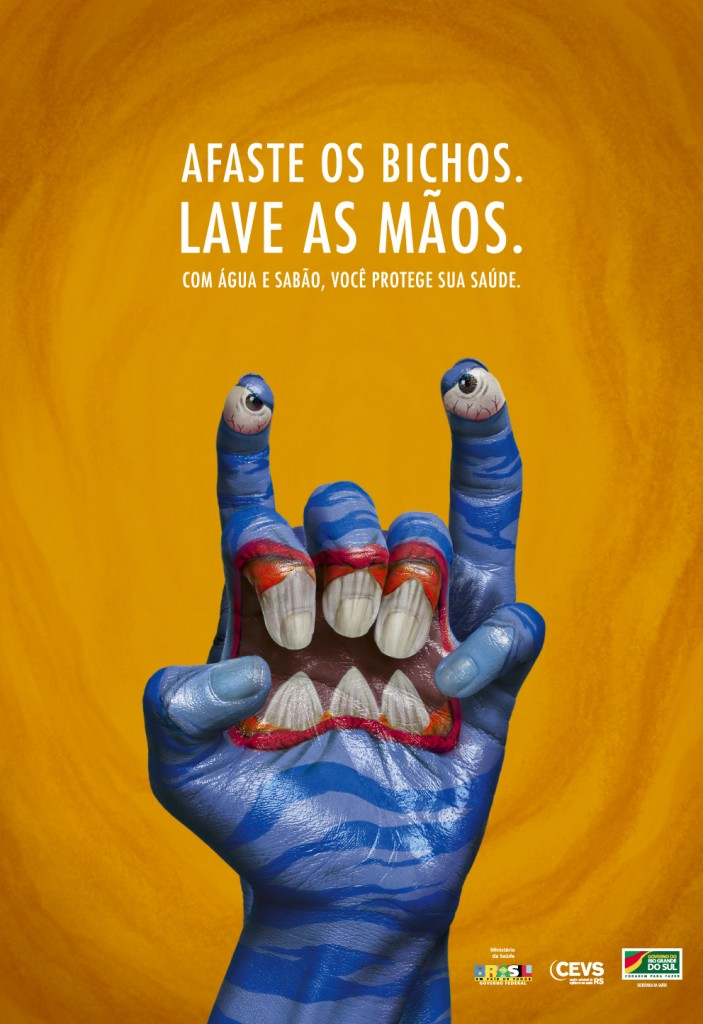
\includegraphics[width=3.27083in,height=4.76432in]{media/image10.jpeg}

a) Qual é o objetivo dessa campanha? O objetivo é orientar a população a
lavar as mãos.

\protect\hypertarget{_Hlk127604103}{}{}\_\_\_\_\_\_\_\_\_\_\_\_\_\_\_\_\_\_\_\_\_\_\_\_\_\_\_\_\_\_\_\_\_\_\_\_\_\_\_\_\_\_\_\_\_\_\_\_\_\_\_\_\_\_\_\_\_\_\_\_\_\_\_\_

\_\_\_\_\_\_\_\_\_\_\_\_\_\_\_\_\_\_\_\_\_\_\_\_\_\_\_\_\_\_\_\_\_\_\_\_\_\_\_\_\_\_\_\_\_\_\_\_\_\_\_\_\_\_\_\_\_\_\_\_\_\_\_\_

b) Você acha importante lavar as mãos? Por quê?

Resposta pessoal. Espera-se que os alunos respondam que sim, porque é um
hábito que pode impedir a propagação de diversas doenças.

\_\_\_\_\_\_\_\_\_\_\_\_\_\_\_\_\_\_\_\_\_\_\_\_\_\_\_\_\_\_\_\_\_\_\_\_\_\_\_\_\_\_\_\_\_\_\_\_\_\_\_\_\_\_\_\_\_\_\_\_\_\_\_\_

\_\_\_\_\_\_\_\_\_\_\_\_\_\_\_\_\_\_\_\_\_\_\_\_\_\_\_\_\_\_\_\_\_\_\_\_\_\_\_\_\_\_\_\_\_\_\_\_\_\_\_\_\_\_\_\_\_\_\_\_\_\_\_\_

\_\_\_\_\_\_\_\_\_\_\_\_\_\_\_\_\_\_\_\_\_\_\_\_\_\_\_\_\_\_\_\_\_\_\_\_\_\_\_\_\_\_\_\_\_\_\_\_\_\_\_\_\_\_\_\_\_\_\_\_\_\_\_\_

\_\_\_\_\_\_\_\_\_\_\_\_\_\_\_\_\_\_\_\_\_\_\_\_\_\_\_\_\_\_\_\_\_\_\_\_\_\_\_\_\_\_\_\_\_\_\_\_\_\_\_\_\_\_\_\_\_\_\_\_\_\_\_\_

c) O que é preciso usar para lavar as mãos e proteger a saúde?

Água e sabão.

\_\_\_\_\_\_\_\_\_\_\_\_\_\_\_\_\_\_\_\_\_\_\_\_\_\_\_\_\_\_\_\_\_\_\_\_\_\_\_\_\_\_\_\_\_\_\_\_\_\_\_\_\_\_\_\_\_\_\_\_\_\_\_\_

\_\_\_\_\_\_\_\_\_\_\_\_\_\_\_\_\_\_\_\_\_\_\_\_\_\_\_\_\_\_\_\_\_\_\_\_\_\_\_\_\_\_\_\_\_\_\_\_\_\_\_\_\_\_\_\_\_\_\_\_\_\_\_\_

d) O que a imagem da mão está representando?

A imagem representa os bichos que ficam nas mãos quando não as
higienizamos.

\_\_\_\_\_\_\_\_\_\_\_\_\_\_\_\_\_\_\_\_\_\_\_\_\_\_\_\_\_\_\_\_\_\_\_\_\_\_\_\_\_\_\_\_\_\_\_\_\_\_\_\_\_\_\_\_\_\_\_\_\_\_\_\_

\_\_\_\_\_\_\_\_\_\_\_\_\_\_\_\_\_\_\_\_\_\_\_\_\_\_\_\_\_\_\_\_\_\_\_\_\_\_\_\_\_\_\_\_\_\_\_\_\_\_\_\_\_\_\_\_\_\_\_\_\_\_\_\_

e) \emph{Slogan} é uma frase curta que se destina a prender a atenção do
seu público. Qual é \emph{o slogan} dessa campanha?

Afaste os bichos. Lave as mãos.

\_\_\_\_\_\_\_\_\_\_\_\_\_\_\_\_\_\_\_\_\_\_\_\_\_\_\_\_\_\_\_\_\_\_\_\_\_\_\_\_\_\_\_\_\_\_\_\_\_\_\_\_\_\_\_\_\_\_\_\_\_\_\_\_

\_\_\_\_\_\_\_\_\_\_\_\_\_\_\_\_\_\_\_\_\_\_\_\_\_\_\_\_\_\_\_\_\_\_\_\_\_\_\_\_\_\_\_\_\_\_\_\_\_\_\_\_\_\_\_\_\_\_\_\_\_\_\_\_

f) Assinale as frases que mostram características que podem ser
observadas no \emph{slogan} do cartaz.

( ) Frase longa com excesso de informação.

( x ) Frase curta e de fácil memorização.

( x ) Letras com destaque, para chamar a atenção do leitor.

( ) Letras sem nenhum destaque.

\subsubsection{3.}\label{section-41}

Forme dupla com um colega e criem outro \emph{slogan} para essa
campanha. Registre o resultado no espaço a seguir.

Lembre os alunos de fazerem uso do imperativo nas formas verbais
utilizadas como recurso para convencer o leitor.

\begin{longtable}[]{@{}l@{}}
\toprule
\begin{minipage}[t]{0.97\columnwidth}\raggedright\strut
\_\_\_\_\_\_\_\_\_\_\_\_\_\_\_\_\_\_\_\_\_\_\_\_\_\_\_\_\_\_\_\_\_\_\_\_\_\_\_\_\_\_\_\_\_\_\_\_\_\_\_\_\_\_\_\_\_\_\_\_\_\_\_

\_\_\_\_\_\_\_\_\_\_\_\_\_\_\_\_\_\_\_\_\_\_\_\_\_\_\_\_\_\_\_\_\_\_\_\_\_\_\_\_\_\_\_\_\_\_\_\_\_\_\_\_\_\_\_\_\_\_\_\_\_\_\_

\_\_\_\_\_\_\_\_\_\_\_\_\_\_\_\_\_\_\_\_\_\_\_\_\_\_\_\_\_\_\_\_\_\_\_\_\_\_\_\_\_\_\_\_\_\_\_\_\_\_\_\_\_\_\_\_\_\_\_\_\_\_\_

\_\_\_\_\_\_\_\_\_\_\_\_\_\_\_\_\_\_\_\_\_\_\_\_\_\_\_\_\_\_\_\_\_\_\_\_\_\_\_\_\_\_\_\_\_\_\_\_\_\_\_\_\_\_\_\_\_\_\_\_\_\_\_

\_\_\_\_\_\_\_\_\_\_\_\_\_\_\_\_\_\_\_\_\_\_\_\_\_\_\_\_\_\_\_\_\_\_\_\_\_\_\_\_\_\_\_\_\_\_\_\_\_\_\_\_\_\_\_\_\_\_\_\_\_\_\_\strut
\end{minipage}\tabularnewline
\bottomrule
\end{longtable}

\subsubsection{4.}\label{section-42}

Encontre no caça-palavras a seguir palavras que representam
características do texto publicitário.

\begin{itemize}
\item
  CONVENCER
\item
  LOGOMARCA
\item
  SLOGAN
\item
  TÍTULO
\end{itemize}

\begin{longtable}[]{@{}llllllllllll@{}}
\toprule
K & T & R & S & E & Y & A & E & T & E & T & F\tabularnewline
\midrule
\endhead
P & D & A & T & S & T & O & O & E & E & U & S\tabularnewline
A & T & P & I & Í & E & H & N & E & C & P & P\tabularnewline
S & E & I & A & D & T & S & T & M & E & C & L\tabularnewline
A & A & A & G & S & R & U & C & N & D & O & A\tabularnewline
M & T & O & W & I & E & S & L & E & G & N & U\tabularnewline
T & S & C & T & U & R & N & A & O & A & V & T\tabularnewline
E & P & N & O & R & T & A & M & A & D & E & N\tabularnewline
O & P & S & L & O & G & A & N & T & A & N & E\tabularnewline
E & H & O & S & A & R & I & E & T & B & C & O\tabularnewline
N & W & P & E & C & N & W & R & E & T & E & C\tabularnewline
H & Y & B & A & R & Y & U & O & I & T & R & S\tabularnewline
\bottomrule
\end{longtable}

\subsubsection{5. }\label{section-43}

Leia, agora, outro anúncio de campanha publicitária.

\url{https://caem.ba.gov.br/ver_noticias.php?note=95}

Arte: circular em magenta a frase Doe um brinquedo, ganhe um sorriso!

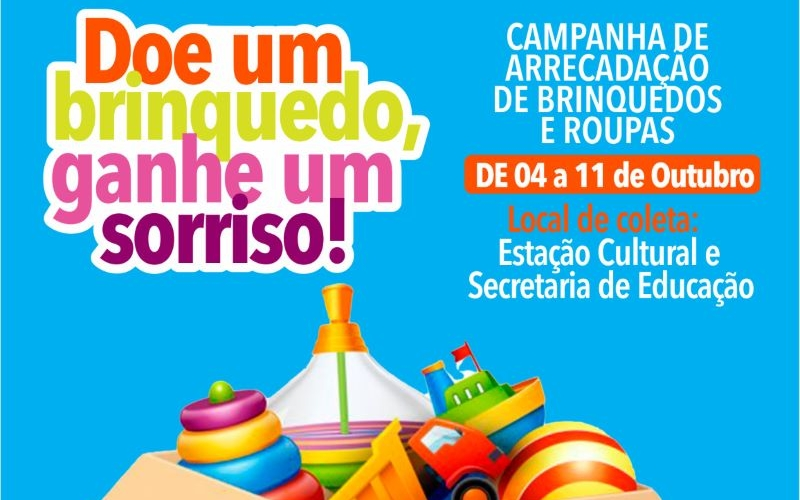
\includegraphics[width=5.12500in,height=3.20313in]{media/image11.jpeg}

a) Qual é o objetivo dessa campanha?

É uma campanha para arrecadação de brinquedos e roupas.

\protect\hypertarget{_Hlk127709586}{}{}\_\_\_\_\_\_\_\_\_\_\_\_\_\_\_\_\_\_\_\_\_\_\_\_\_\_\_\_\_\_\_\_\_\_\_\_\_\_\_\_\_\_\_\_\_\_\_\_\_\_\_\_\_\_\_\_\_\_\_\_\_\_\_\_

\_\_\_\_\_\_\_\_\_\_\_\_\_\_\_\_\_\_\_\_\_\_\_\_\_\_\_\_\_\_\_\_\_\_\_\_\_\_\_\_\_\_\_\_\_\_\_\_\_\_\_\_\_\_\_\_\_\_\_\_\_\_\_\_

b) Circule no cartaz o \emph{slogan} da campanha.

Os alunos devem circular a frase ``Doe um brinquedo, ganhe um
sorriso!''.

c) Onde serão coletados os brinquedos e as roupas?

Na Estação Cultural e Secretaria de Educação.

\_\_\_\_\_\_\_\_\_\_\_\_\_\_\_\_\_\_\_\_\_\_\_\_\_\_\_\_\_\_\_\_\_\_\_\_\_\_\_\_\_\_\_\_\_\_\_\_\_\_\_\_\_\_\_\_\_\_\_\_\_\_\_\_

\_\_\_\_\_\_\_\_\_\_\_\_\_\_\_\_\_\_\_\_\_\_\_\_\_\_\_\_\_\_\_\_\_\_\_\_\_\_\_\_\_\_\_\_\_\_\_\_\_\_\_\_\_\_\_\_\_\_\_\_\_\_\_\_

d) Em sua opinião, por que doar brinquedos garantem sorrisos?

\begin{quote}
Resposta pessoal. Aproveite o momento e explique aos alunos que doar é
um ato de amor ao próximo e, também, evita o acúmulo, além, de fazer a
alegria das crianças que vão recebê-los.
\end{quote}

\_\_\_\_\_\_\_\_\_\_\_\_\_\_\_\_\_\_\_\_\_\_\_\_\_\_\_\_\_\_\_\_\_\_\_\_\_\_\_\_\_\_\_\_\_\_\_\_\_\_\_\_\_\_\_\_\_\_\_\_\_\_\_\_

\_\_\_\_\_\_\_\_\_\_\_\_\_\_\_\_\_\_\_\_\_\_\_\_\_\_\_\_\_\_\_\_\_\_\_\_\_\_\_\_\_\_\_\_\_\_\_\_\_\_\_\_\_\_\_\_\_\_\_\_\_\_\_\_

\subsection{Treino}\label{treino-3}

\subsubsection{1.}\label{section-44}

Leia o cartaz de conscientização para responder à questão. (Fácil)

https://www.bombinhas.sc.gov.br/noticias/ver/2014/11/campanha-de-vacinacao-contra-sarampo-e-paralisia-infantil-inicia-neste-sabado

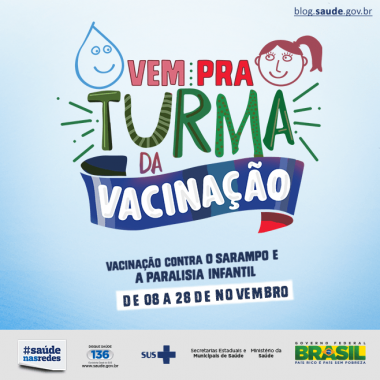
\includegraphics[width=3.95833in,height=3.95833in]{media/image12.png}

Disponível em:
\url{https://www.bombinhas.sc.gov.br/noticias/ver/2014/11/campanha-de-vacinacao-contra-sarampo-e-paralisia-infantil-inicia-neste-sabado}.
Acesso em: 18 fev. 2023.

Ao ler o cartaz, compreende-se que ele traz uma campanha sobre a
importância

(A) da desenhar.

(B) de ter a sua própria ``turma'', ou seja, seus amigos.

(C) da amizade e das brincadeiras com os amigos.

(D) da vacinação contra o sarampo e a paralisia infantil.

SaebD7 - Relacionar, na compreensão do texto, informações textuais com
conhecimentos de senso comum.

BNCC: EF03LP19: Identificar e discutir o propósito do uso de recursos de
persuasão (cores, imagens, escolha de palavras, jogo de palavras,
tamanho de letras) em textos publicitários e de propaganda, como
elementos de convencimento.

.

(A) Incorreta. Embora haja a presença de desenhos no anúncio, esse não é
esse o objetivo da campanha, visto que a conscientização é referente à
vacinação.

(B) Incorreta. A ``turma da vacinação'' é referente à conscientização
sobre a necessidade de se vacinar contra doenças específicas, não em
relação à importância de ter amizades.

(C) Incorreta. A finalidade da campanha é promover a conscientização da
importância da vacinação contra o sarampo e a paralisia infantil.

(D) Correta. No cartaz, compreende-se que os elementos verbais e não
verbais apontam para a importância da vacinação contra o sarampo e a
paralisia infantil, dado o anúncio ``Vacinação contra o sarampo e a
paralisia infantil'', bem como o slogan ``Vem pra turma da vacinação''.

\subsubsection{2. }\label{section-45}

Observe o cartaz da campanha, atentando-se ao \emph{slogan}. (Médio)

https://i.pinimg.com/originals/73/ce/78/73ce78802f6062e3f50dfe73c65931b4.jpg

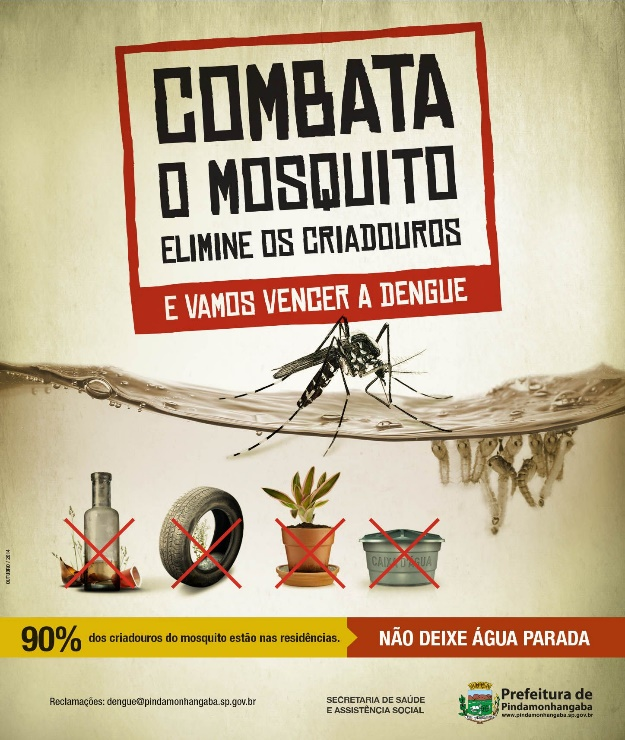
\includegraphics[width=2.84375in,height=3.36642in]{media/image13.jpeg}

Qual é o \emph{slogan} dessa campanha de conscientização?

(A) Combata o mosquito elimine, os criadouros.

(B) E vamos combater a dengue.

(C) Não deixe água parada.

(D) Prefeitura de Pindamonhangaba.

SaebD7 - Relacionar, na compreensão do texto, informações textuais com
conhecimentos de senso comum.

BNCC: EF03LP19: Identificar e discutir o propósito do uso de recursos de
persuasão (cores, imagens, escolha de palavras, jogo de palavras,
tamanho de letras) em textos publicitários e de propaganda, como
elementos de convencimento.

.

(A) Correta. O \emph{slogan} é uma frase de efeito para chamar a atenção
do leitor, relacionada ao tema da campanha. Assim, ao ler o cartaz,
compreende-se que o slogan dele é

``Combata o mosquito elimine, os criadouros''.

(B) Incorreta. ``E vamos combater a dengue'' é a ação proposta pelo
cartaz, não a frase de efeito para chamar a atenção do leitor.

(C) Incorreta. As frases é uma ação que a população deve fazer para
evitar a criação do mosquito da dengue, não é, portanto, o \emph{slogan}
da campanha.

(D) Incorreta. Prefeitura de Pindamonhangaba é a instituição responsável
pela veiculação do anúncio.

\subsubsection{3. }\label{section-46}

Leia o cartaz de campanha de conscientização, observando as imagens e o
texto. (Difícil)

https://vitalvereador.wordpress.com/2012/01/29/campanha-vamos-tirar-o-planeta-do-sufoco/

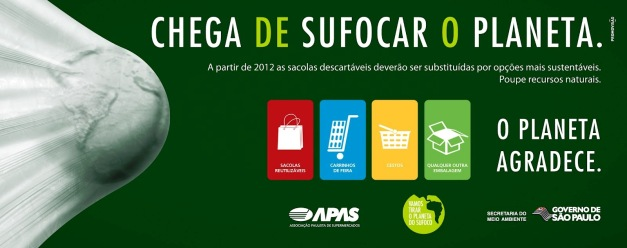
\includegraphics[width=6.14514in,height=2.43088in]{media/image14.jpeg}

Disponível em:
\url{https://vitalvereador.wordpress.com/2012/01/29/campanha-vamos-tirar-o-planeta-do-sufoco/}.
Acesso em: 18 fev. 2023.

Considerando a relação entre as imagens e o texto verbal, podemos
perceber que

(A) as sacolas plásticas prejudicam o meio ambiente.

(B) os carrinhos de feira são melhores que as sacolas reutilizáveis.

(C) a produção das embalagens reutilizáveis custa mais caro.

(D) o planeta foi prejudicado pelos cestos e carrinhos de feira.

Saeb: D10 - Diferenciar, por comparação ou identificação de
características, textos de diferentes gêneros (notícia x narrativa
ficcional; notícia x texto expositivo de outras áreas; propaganda x
anúncio).

BNCC: EF03LP19: Identificar e discutir o propósito do uso de recursos de
persuasão (cores, imagens, escolha de palavras, jogo de palavras,
tamanho de letras) em textos publicitários e de propaganda, como
elementos de convencimento.

.

(A) Correta. Ao observar o Planeta Terra envolto em uma sacola plástica,
pode-se deduzir usar menos sacolas plásticas, visto que o descarte delas
causa danos ao meio ambiente.

(B) Incorreta. O texto apresenta quatro alternativas ao uso de sacolas,
sem mencionar qual é a melhor.

(C) Incorreta. O anúncio traz informações de que é melhor usar
embalagens reutilizáveis, não fazendo restrições a esse tipo de produto.

(D) Incorreta. O planeta foi prejudicado pela utilização de sacolas
plásticas.

\section{Módulo 5}\label{muxf3dulo-5}

Orientação para o professor: Neste módulo, espera-se que os alunos
localizem informações explícitas no poema; identifiquem a função social
do texto, reconhecendo

A sua função, onde circula, quem o produziu e a quem se destina;
reconheçam características do poema, como estrofes e versos, rimas nos
versos; notem a relação entre textos; reconheçam o sentido figurado de
palavras e expressões utilizadas no poema; infiram o sentido de
palavras, com base no contexto de trecho de texto.

\textbf{Habilidades BNCC: EF35LP27; EF35LP31}

\textbf{Habilidades SAEB}

\textbf{- Reconhecer diferentes modos de organização composicional de
textos em versos.}

\textbf{- Analisar a construção de sentidos de textos em versos com base
em seus elementos constitutivos.}

\subsection{Conteúdo}\label{conteuxfado-4}

\href{https://www.istockphoto.com/br/vetor/escritora-cria-poesia-com-pena-no-papel-gm1346126990-423980947?utm_source=pixabay\&utm_medium=affiliate\&utm_campaign=SRP_vector_sponsored\&utm_content=https\%3A\%2F\%2Fpixabay.com\%2Fpt\%2Fvectors\%2Fsearch\%2Fpoema\%2F\%3Fmanual_search\%3D1\&utm_term=poema}{https://www.istockphoto.com/br/vetor/escritora-cria-poesia-com-pena-no-papel-gm1346126990-423980947?utm\_source=pixabay\&utm\_medium=affiliate\&utm\_campaign=SRP\_vector\_sponsored\&utm\_content=https\%3A\%2F\%2Fpixabay.com\%2Fpt\%2Fvectors\%2Fsearch\%2Fpoema\%2F\%3Fmanual\_search\%3D1\&utm\_term=poema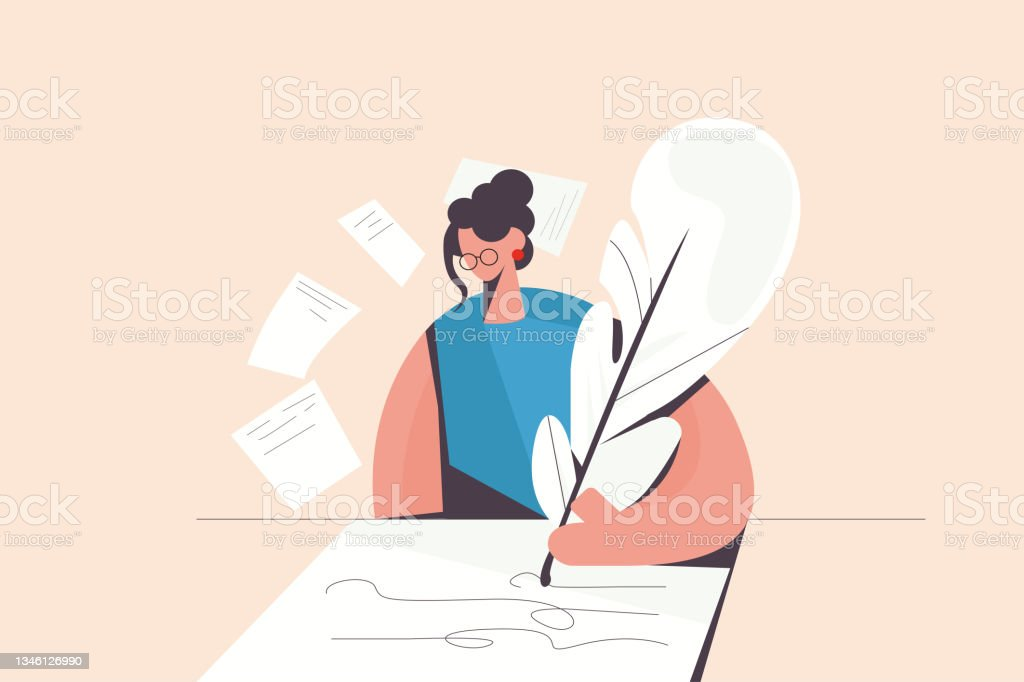
\includegraphics[width=4.80139in,height=3.19792in]{media/image15.jpeg}}

\textbf{POEMAS}

\textbf{Poema} consiste em um gênero textual que apresenta estrutura em
versos. Sua principal característica é explorar a linguagem de modo
diferenciado, isto é, utiliza a sonoridade das palavras (apresenta rima,
repetição de sons e ritmo) e utiliza termos e expressões no sentido
figurado: com significado diferente daquele que normalmente apresenta.

\textbf{Verso} é cada uma das linhas que compõem o poema. Alguns poemas
podem ser organizados em conjuntos de versos separados por uma linha em
branco. Esses conjuntos de versos denominam-se \textbf{estrofes}. Nas
estrofes, pode ou não haver rimas entre os versos que as compõem.

Em um texto poético, é necessário fazer a distinção entre o poeta, ou
seja, o escritor, do ``eu'' que fala no texto. Em texto narrativos, por
exemplo, quem dá a voz denomina-se narrador, nos poemas, a voz
expressada denomina-se ``eu lírico''. Nos poemas, é possível expressar
sentimentos, ideias e emoções, o que permite envolver o leitor e
despertar nele as mais diferentes sensações. Além disso, a escolha
cuidadosa das palavras e a forma como são organizadas no texto conferem
beleza ao poema e também são responsáveis por atrair o interesse dos
leitores.

O poema pode apresentar as mais variadas estruturas. A mais comum tem
estrutura na vertical, isto é, um verso embaixo do outro. Os versos
poderão ser agrupados em estrofes, e as estrofes são, geralmente,
separadas por uma linha em branco.

É o poeta quem escolhe o título e o tamanho do poema. É bom lembrar que
as escolhas (assunto, título, recursos poéticos etc.) realizadas pelo
poeta levam em consideração que, normalmente, o texto poético procura
sensibilizar o leitor, provocando sentimentos e emoções no momento da
leitura.

Na elaboração do texto, o poeta se utiliza de muitos recursos poéticos,
como rima, recursos visuais e sonoros, imagens poéticas ou
\textbf{onomatopeias} (imitação de sons utilizando palavras como
tchibum, trim trim, tique-taque, toc-toc, entre outras.

\subsection{Atividades}\label{atividades-4}

\subsubsection{1. }\label{section-47}

Leia o poema a seguir. Em seguida, responda às questões propostas.

Inserir imagem do relógio ao lado do poema.
https://www.pexels.com/pt-br/foto/relogio-analogico-preto-e-amarelo-3283142/

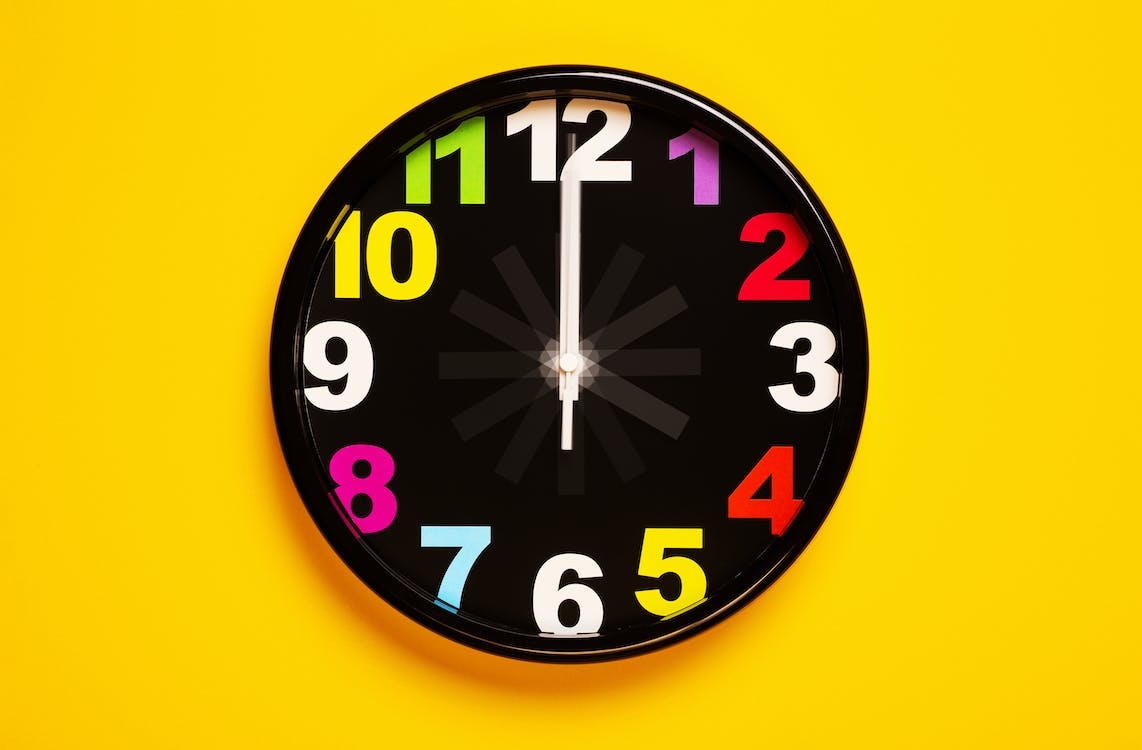
\includegraphics[width=4.46875in,height=2.93485in]{media/image16.jpeg}

\textbf{O relógio}

Preso à parede, sozinho \emph{lá},

Alvo dos olhos de toda \emph{gente},

Minutos e horas, \emph{eternamente},

Alma do tempo, batendo \emph{está}.

Na intimidade de todo \emph{lar}

Se as alegrias são \emph{verdadeiras},

As horas correm, voam \emph{ligeiras}

Para a ventura não \emph{demorar}.

Gelam os risos, e quando \emph{enfim}

Dor ou tristeza nos olhos \emph{chora},

Calmo, o relógio para e \emph{demora},

A hora parece que não tem \emph{fim}.

JÚLIA, Francisca. ``O relógio''. \textbf{Alma Infantil} (Versos para
usos das escolas). São Paulo/Rio de Janeiro: Editora Livraria Magalhães.
1912, p. 25-26. Disponível em:
\textless{}https://digital.bbm.usp.br/bitstream/bbm/4556/1/033579\_COMPLETO.pdf\textgreater{}.
Acesso em: 19 fev. jan. 2023.

ligeiras: rápidas, velozes.

ventura: felicidade.

a) Qual é ó título do poema? O relógio

\_\_\_\_\_\_\_\_\_\_\_\_\_\_\_\_\_\_\_\_\_\_\_\_\_\_\_\_\_\_\_\_\_\_\_\_\_\_\_\_\_\_\_\_\_\_\_\_\_\_\_\_\_\_\_\_\_\_\_\_\_\_\_\_

\_\_\_\_\_\_\_\_\_\_\_\_\_\_\_\_\_\_\_\_\_\_\_\_\_\_\_\_\_\_\_\_\_\_\_\_\_\_\_\_\_\_\_\_\_\_\_\_\_\_\_\_\_\_\_\_\_\_\_\_\_\_\_\_

b) Quem escreveu o poema? Francisca Júlia

\_\_\_\_\_\_\_\_\_\_\_\_\_\_\_\_\_\_\_\_\_\_\_\_\_\_\_\_\_\_\_\_\_\_\_\_\_\_\_\_\_\_\_\_\_\_\_\_\_\_\_\_\_\_\_\_\_\_\_\_\_\_\_\_

\_\_\_\_\_\_\_\_\_\_\_\_\_\_\_\_\_\_\_\_\_\_\_\_\_\_\_\_\_\_\_\_\_\_\_\_\_\_\_\_\_\_\_\_\_\_\_\_\_\_\_\_\_\_\_\_\_\_\_\_\_\_\_\_

c) Em que livro esse poema foi publicado? Alma infantil.

Atente os alunos para a referência no fim do texto, que apresenta as
seguintes informações: nome do autor, nome da obra, editora que publicou
o livro (local e nome), ano de publicação da obra, número da página da
qual o poema foi retirado e \emph{link} de onde está na internet.

\_\_\_\_\_\_\_\_\_\_\_\_\_\_\_\_\_\_\_\_\_\_\_\_\_\_\_\_\_\_\_\_\_\_\_\_\_\_\_\_\_\_\_\_\_\_\_\_\_\_\_\_\_\_\_\_\_\_\_\_\_\_\_\_

\_\_\_\_\_\_\_\_\_\_\_\_\_\_\_\_\_\_\_\_\_\_\_\_\_\_\_\_\_\_\_\_\_\_\_\_\_\_\_\_\_\_\_\_\_\_\_\_\_\_\_\_\_\_\_\_\_\_\_\_\_\_\_\_

\begin{enumerate}
\def\labelenumi{\alph{enumi})}
\item
  De acordo com o poema, se as alegrias são verdadeiras, as horas passam
\end{enumerate}

( ) lentamente.

( x ) rapidamente.

\begin{enumerate}
\def\labelenumi{\alph{enumi})}
\item
  Mas quando os olhos choram, as horas passam
\end{enumerate}

( x ) devagar.

( ) ligeiro.

\subsubsection{2. }\label{section-48}

Leia este verbete de dicionário.

\begin{quote}
https://aulete.com.br/gelar
\end{quote}

\begin{longtable}[]{@{}l@{}}
\toprule
\begin{minipage}[t]{0.97\columnwidth}\raggedright\strut
\textbf{Gelar}

\textbf{(ge.lar)}

\textbf{v.}

\textbf{1. Esfriar(-se) muito. {[}td.: Gelou o suco antes de servir.{]}
{[}int.: Estava sem meias, seus pés gelaram.{]}}\strut
\end{minipage}\tabularnewline
\bottomrule
\end{longtable}

\begin{quote}
Disponível em: https://aulete.com.br/gelar. Acesso em: 19 fev. 2023.
\end{quote}

\begin{enumerate}
\def\labelenumi{\alph{enumi})}
\item
  Agora, releia o trecho a seguir:
\end{enumerate}

\begin{longtable}[]{@{}l@{}}
\toprule
\begin{minipage}[t]{0.97\columnwidth}\raggedright\strut
Gelam os risos, e quando enfim

Dor ou tristeza nos olhos chora,\strut
\end{minipage}\tabularnewline
\bottomrule
\end{longtable}

\begin{itemize}
\item
  Em sua opinião, a palavra \textbf{gelam} apresenta o mesmo significado
  apresentado no verbete? Justifique sua resposta.
\end{itemize}

Explique aos alunos que, no poema, a palavra \textbf{gelam} foi
utilizada em sentido figurado: apresenta relação de proximidade com o
sentido primitivo ou extensão do significado original.

\_\_\_\_\_\_\_\_\_\_\_\_\_\_\_\_\_\_\_\_\_\_\_\_\_\_\_\_\_\_\_\_\_\_\_\_\_\_\_\_\_\_\_\_\_\_\_\_\_\_\_\_\_\_\_\_\_\_\_\_\_\_\_\_

\_\_\_\_\_\_\_\_\_\_\_\_\_\_\_\_\_\_\_\_\_\_\_\_\_\_\_\_\_\_\_\_\_\_\_\_\_\_\_\_\_\_\_\_\_\_\_\_\_\_\_\_\_\_\_\_\_\_\_\_\_\_\_\_

\_\_\_\_\_\_\_\_\_\_\_\_\_\_\_\_\_\_\_\_\_\_\_\_\_\_\_\_\_\_\_\_\_\_\_\_\_\_\_\_\_\_\_\_\_\_\_\_\_\_\_\_\_\_\_\_\_\_\_\_\_\_\_\_

\_\_\_\_\_\_\_\_\_\_\_\_\_\_\_\_\_\_\_\_\_\_\_\_\_\_\_\_\_\_\_\_\_\_\_\_\_\_\_\_\_\_\_\_\_\_\_\_\_\_\_\_\_\_\_\_\_\_\_\_\_\_\_\_

\subsubsection{3. }\label{section-49}

\textbf{Verso} é cada linha de um poema. \textbf{Estrofe} é cada
conjunto de versos. Quantas estrofes e quantos versos há no poema?

\begin{quote}
O poema tem 3 estrofes e 12 versos.

\_\_\_\_\_\_\_\_\_\_\_\_\_\_\_\_\_\_\_\_\_\_\_\_\_\_\_\_\_\_\_\_\_\_\_\_\_\_\_\_\_\_\_\_\_\_\_\_\_\_\_\_\_\_\_\_\_\_\_\_\_\_\_\_

\_\_\_\_\_\_\_\_\_\_\_\_\_\_\_\_\_\_\_\_\_\_\_\_\_\_\_\_\_\_\_\_\_\_\_\_\_\_\_\_\_\_\_\_\_\_\_\_\_\_\_\_\_\_\_\_\_\_\_\_\_\_\_\_

\_\_\_\_\_\_\_\_\_\_\_\_\_\_\_\_\_\_\_\_\_\_\_\_\_\_\_\_\_\_\_\_\_\_\_\_\_\_\_\_\_\_\_\_\_\_\_\_\_\_\_\_\_\_\_\_\_\_\_\_\_\_\_\_
\end{quote}

\subsubsection{4. }\label{section-50}

Sublinhe os pares de palavras que rimam no poema.

\subsubsection{5. }\label{section-51}

Leia ``Uma amiguinha'', poema sobre Resedá, uma gatinha de estimação
bastante dengosa.

Promova uma leitura expressiva desse poema, desse modo, estará
desenvolvendo a fluência, identificação e apreciação de textos em
versos.

Inserir imagem ao lado do poema:
https://pixabay.com/pt/vectors/gato-scottish-fold-gatinho-gatinha-7753428/

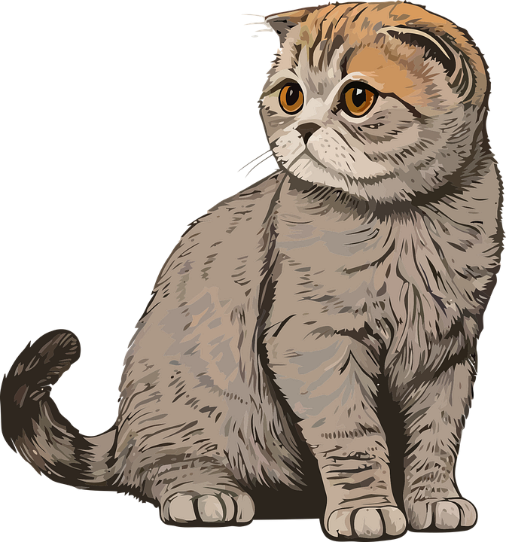
\includegraphics[width=2.29455in,height=2.45833in]{media/image17.png}

\textbf{Uma amiguinha}

É inteligente e graciosa;

Mais limpa, que ela, não há:

Focinhito cor-de-rosa,

E chama-se Resedá.

{[}...{]}

Gosta do sol, ama as flores,

Corre por todo o jardim,

E tem, no dorso, em três cores,

A maciez do cetim.

{[}...{]}

Mas é boazinha e correta;

Não provoca ásperos tratos;

Somente mostra-se inquieta,

Se escuta rumor de ratos.

ROLIM, Zalina. Uma amiguinha. In: Livro das Crianças. Disponível em:

\url{https://www.unicamp.br/iel/memoria/Ensaios/LiteraturaInfantil/10Zalina.htm}.
Acesso em: 11 fev.

2020.

Focinhito: focinho.

Dorso: costas.

Cetim: tipo de tecido muito macio.

Inquieta: agitada.

Rumor: ruído.

a) O título do texto é ``Uma amiguinha''. Que é a amiguinha?

A amiguinha é a gatinha Resedá.

\_\_\_\_\_\_\_\_\_\_\_\_\_\_\_\_\_\_\_\_\_\_\_\_\_\_\_\_\_\_\_\_\_\_\_\_\_\_\_\_\_\_\_\_\_\_\_\_\_\_\_\_\_\_\_\_\_\_\_\_\_\_\_\_

\_\_\_\_\_\_\_\_\_\_\_\_\_\_\_\_\_\_\_\_\_\_\_\_\_\_\_\_\_\_\_\_\_\_\_\_\_\_\_\_\_\_\_\_\_\_\_\_\_\_\_\_\_\_\_\_\_\_\_\_\_\_\_\_

b) Quantas estrofes e quantos versos há no poema? Há 3 estrofes e 12
versos.

\_\_\_\_\_\_\_\_\_\_\_\_\_\_\_\_\_\_\_\_\_\_\_\_\_\_\_\_\_\_\_\_\_\_\_\_\_\_\_\_\_\_\_\_\_\_\_\_\_\_\_\_\_\_\_\_\_\_\_\_\_\_\_\_

\_\_\_\_\_\_\_\_\_\_\_\_\_\_\_\_\_\_\_\_\_\_\_\_\_\_\_\_\_\_\_\_\_\_\_\_\_\_\_\_\_\_\_\_\_\_\_\_\_\_\_\_\_\_\_\_\_\_\_\_\_\_\_\_

c) Escreva uma rima presente no poema. Sugestão de resposta: É
inteligente e graciosa; / Focinhito cor-de-rosa

\_\_\_\_\_\_\_\_\_\_\_\_\_\_\_\_\_\_\_\_\_\_\_\_\_\_\_\_\_\_\_\_\_\_\_\_\_\_\_\_\_\_\_\_\_\_\_\_\_\_\_\_\_\_\_\_\_\_\_\_\_\_\_\_

\_\_\_\_\_\_\_\_\_\_\_\_\_\_\_\_\_\_\_\_\_\_\_\_\_\_\_\_\_\_\_\_\_\_\_\_\_\_\_\_\_\_\_\_\_\_\_\_\_\_\_\_\_\_\_\_\_\_\_\_\_\_\_\_

d) Marque, a seguir, as palavras que rimam com \textbf{graciosa} e
\textbf{cor-de-rosa}.

( x ) misteriosa ( ) mimada ( x ) sedosa ( ) quietinha

e) Releia o trecho do poema.

\begin{longtable}[]{@{}l@{}}
\toprule
\begin{minipage}[t]{0.97\columnwidth}\raggedright\strut
Mas é boazinha e correta;

Não provoca ásperos tratos;

Somente mostra-se inquieta,

Se escuta rumor de ratos.\strut
\end{minipage}\tabularnewline
\bottomrule
\end{longtable}

\begin{itemize}
\item
  Que outra palavra poderia substituir a palavra \textbf{ratos} e, ainda
  assim, manter a rima do poema? Resposta pessoal. Sugestões de
  resposta: pratos, sapatos, patos, etc.
\end{itemize}

\begin{quote}
\_\_\_\_\_\_\_\_\_\_\_\_\_\_\_\_\_\_\_\_\_\_\_\_\_\_\_\_\_\_\_\_\_\_\_\_\_\_\_\_\_\_\_\_\_\_\_\_\_\_\_\_\_\_\_\_\_\_\_\_\_\_\_\_

\_\_\_\_\_\_\_\_\_\_\_\_\_\_\_\_\_\_\_\_\_\_\_\_\_\_\_\_\_\_\_\_\_\_\_\_\_\_\_\_\_\_\_\_\_\_\_\_\_\_\_\_\_\_\_\_\_\_\_\_\_\_\_\_
\end{quote}

\subsection{Treino}\label{treino-4}

\subsubsection{1. }\label{section-52}

\begin{quote}
(Fácil) Leia um trecho da canção \textbf{Sítio do pica-pau amarelo}.

Sítio do pica-pau amarelo

Marmelada de banana

bananada de goiaba

goiabada de marmelo

{[}...{]}

GIL, Gilberto. ``Sítio do Pica-Pau Amarelo''. Intérprete: Gilberto Gil.
In: Kaya N'Gan Daya: Ao vivo. Rio de Janeiro: Warner Music, 2003. CD,
faixa 16.

A palavra destacada no texto rima com todas as palavras listadas em

(A) goiabada -- namorada -- madrugada.

(B) goiabada -- martelo -- salada.

(C) privada -- picada -- moela.

(D) limonada -- bala -- gargalhada.

Saeb D6 - Utilizar informações oferecidas por um glossário, verbete de
dicionário ou texto informativo na compreensão ou interpretação do
texto.

BNCC: EF35LP27: Ler e compreender, com certa autonomia, textos em
versos, explorando rimas, sons e jogos de palavras, imagens poéticas
(sentidos figurados) e recursos visuais e sonoros.

(A) Correta. Deve-se notar a terminação da palavra marmelada e
identificar nas alternativas em qual delas todas as palavras têm a mesma
terminação.

(B) Incorreta. Martelo não faz rima com marmelada.

(C) Incorreta. Moela não faz rima com marmelada.

(D) Incorreta. Bala não faz rima com marmelada.
\end{quote}

\subsubsection{2. }\label{section-53}

\begin{quote}
(Médio) Leia o trecho do poema ``Infância'', de Casimiro de Abreu.

Infância

{[}...{]}

Ó anjo da loura trança,

És criança,

A vida começa a rir.

- Vive e folga descansada,

Descuidada

Das tristezas do porvir.

ABREU, Casimiro de. ``Infância''. Disponível em:

www.dominiopublico.gov.br/download/texto/wk000394.pdf. Acesso em: 20
fev. 2023.
\end{quote}

porvir: futuro.

A rima ocorre em:

(A) ``Infância'' e ``Vive e folga descansada''.

(B) ``Ó anjo da loura trança'' e ``A vida começa a rir''.

(C) ``A vida começa a rir'' e ``Das tristezas do porvir''.

(D) ``És criança'' e ``Descuidada''.

Saeb D2 - Inferir uma afirmação implícita num texto.

BNCC: EF35LP27: Ler e compreender, com certa autonomia, textos em
versos, explorando rimas, sons e jogos de palavras, imagens poéticas
(sentidos figurados) e recursos visuais e sonoros.

(A) Incorreta. As palavras ``infância'' e ``descansada'' não apresentam
o mesmo som final.

(B) Incorreta. As palavras ``trança'' e ``rir'' não apresentam o mesmo
som final.

(C) Correta. A rima acontece em versos, como ``A vida começa a rir'' e
``Das tristezas do porvir'', que apresentam o som igual nas últimas
palavras ``rir'' e ``porvir''.

(D) Incorreta. As palavras ``criança'' e ``descuidada'' não apresentam o
mesmo som final.

\subsubsection{3. }\label{section-54}

Leia o poema a seguir.

\textbf{O meu retrato}

Aquele retrato lá:

O corpo, as pernas, o braço,

Sou eu mesmo traço a traço,

Tão parecido ele está.

Acham bonito? talvez...

O nariz ó um pouco chato...

Mas, que importa? é o meu retrato;

Foi o vovô quem o fez.

JULIA, Francisca; SILVA, Julio da. O meu retrato. Alma infantil.
Disponível em:

https://digital.bbm.usp.br/bitstream/bbm/4556/1/033579\_COMPLETO.pdf.
Acesso em: 20 fev. 2023.

Pode-se notar uma rima entre as palavras ``retrato'' e ``chato'', pois

(A) a letra final é igual, ou seja, ``o''.

(B) os sons finais se repetem, isto é, ``-ato''.

(C) a letra ``t'' está presente nas duas palavras.

(D) o som de ``ato'' está no começo da palavra.

Saeb D18 -- Reconhecer o efeito de sentido decorrente da escolha de uma
determinada palavra ou expressão.

BNCC: EF35LP31: Identificar, em textos versificados, efeitos de sentido
decorrentes do uso de recursos rítmicos e sonoros e de metáforas.

(A) Incorreta. Os sons finais das palavras são diferentes.

(B) Correta. Entre ``retrato'' e ``chato'' existe rima, pois ambas
apresentam o mesmo som final ``-ato''.

(C) Incorreta. Não há rima entre as palavras.

(D) Incorreta. O som de ``-ato'' é o que faz a rima entre as palavras,
no entanto, esse som não está no começo de palavra, mas no fim da
palavra, o que caracteriza a rima.

\section{Módulo 6}\label{muxf3dulo-6}

\subsection{Conteúdo}\label{conteuxfado-5}

\textbf{Discursos direto e indireto}

https://pixabay.com/pt/vectors/falar-pessoas-conversa\%c3\%a7\%c3\%a3o-amigo-7647863/

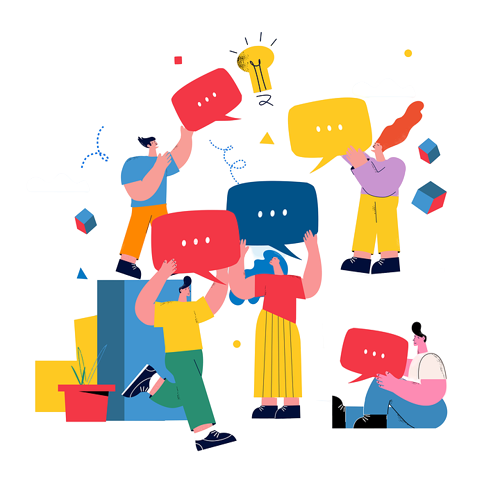
\includegraphics[width=3.01042in,height=3.01042in]{media/image18.png}

~O discurso direto é a transcrição fiel da fala das personagens na
narração, em que não acontece a participação do narrador. Esse tipo de
discurso normalmente é precedido pelo travessão (sinal de pontuação que
indica quando se inicia a fala de uma personagem, quando ocorre mudança
de interlocutores e quando existe mudança para o narrador mediante um
verbo de elocução). No entanto, muitos autores de narração preferem
colocar o discurso direto entre aspas (sinal de pontuação que mostra uma
transcrição ou citação).\\
O discurso direto é iniciado por verbos de elocução, tais como: falar,
dizer, comentar, perguntar, responder, observar, murmurar, exclamar,
gritar, aconselhar etc. Os verbos de elocução são seguidos por dois
pontos (sinal de pontuação).

O discurso direto também pode ser usado para dar voz aos personagens,
propiciando ao leitor notar variadas reações diante dos acontecimentos
que estão sendo narrados. Assim sendo, o discurso direto torna a
narração mais dinâmica e atraente ao leitor.

Na escrita, as marcas do discurso direto são: dois pontos (:), mudança
de linha para novo parágrafo e início da fala com travessão (-).

Exemplo:

\textbf{João disse:}

\textbf{- A Brisa é uma gatinha muito fofa!}

O discurso indireto consiste em uma reprodução do conteúdo das falas dos
personagens, em vez de uma transcrição exata delas, com as palavras do
narrador. Ele atua como intermediário, muitas vezes incluindo também
emoções, reações, sentimentos ou marcas de personalidade do personagem.

Neste caso, a narração é feita na 3ª pessoa. Também pode ser introduzido
por verbos de elocução.

Exemplo:

\textbf{O João disse que a Brisa é uma gatinha muito fofa.}

Agora, vamos treinar!

\subsection{Atividades}\label{atividades-5}

\subsubsection{1. }\label{section-55}

Leia o conto a seguir, de Monteiro Lobato.

\begin{quote}
https://pixabay.com/pt/vectors/tartaruga-animal-desenho-animado-151431/
\end{quote}

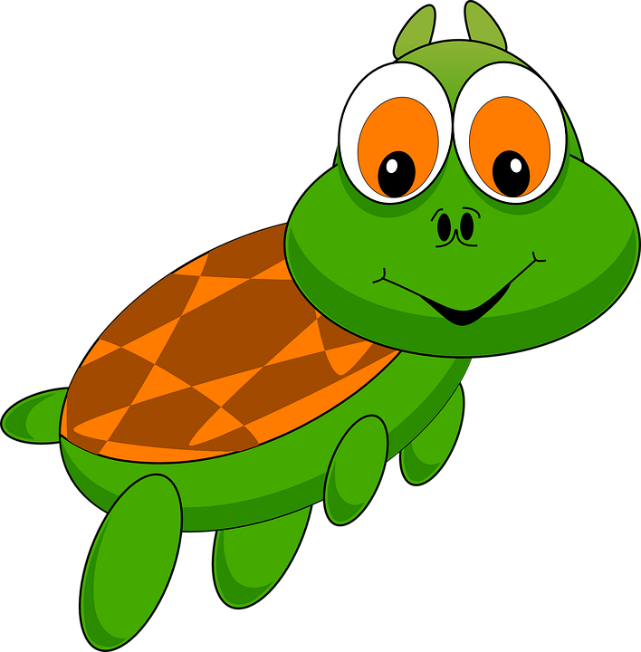
\includegraphics[width=2.90902in,height=2.95828in]{media/image19.png}

\textbf{O cágado na festa do céu}

Certa vez houve uma grande festa no céu, para a qual foram convidados os
bichos da floresta. Todos se encaminharam para lá, e o cágado também ---
mas este era vagaroso demais, de modo que andava, andava e não chegava
nunca.

A festa era só de três dias e o cágado nada de chegar. Desanimado, pediu
a uma garça que o conduzisse às costas. A garça respondeu: "Pois não", e
o cágado montou.

A garça foi subindo, subindo, subindo; de vez em quando perguntava ao
cágado se estava vendo a terra.

--- Estou, sim, mas lá longe.

A garça subia mais e mais.

--- E agora?

--- Agora já não vejo o menor sinalzinho da terra.

A garça, então, que era uma perversa, fez uma reviravolta no ar,
desmontando o cágado. Coitado! Começou a cair com velocidade cada vez
maior. E enquanto caía, murmurava:

\emph{Se eu desta escapar,}

\emph{léu, léu, léu,}

\emph{se eu desta escapar,}

\emph{nunca mais ao céu me deixarei levar.}

Nisto avistou lá embaixo a terra. Gritou:

--- Arredai-vos, pedras e paus, senão eu vos esmagarei! As pedras e paus
se afastaram e o cágado caiu. Mesmo assim arrebentou-se todo, em cem
pedaços.

Deus, que estava vendo tudo, teve dó do coitado. Afinal de contas aquela
desgraça tinha acontecido só porque ele teimou em comparecer à festa do
céu. E Deus juntou outra vez os pedaços.

É por isso que o cágado tem a casca feita de pedacinhos emendados uns
nos outros.

LOBATO, Monteiro. \textbf{O cágado na festa do céu}. Histórias da Tia
Nastácia. Disponível em:
https://www.miniweb.com.br/cantinho/infantil/38/estorias\_miniweb/lobato/historias\_de\_tia\_nastacia.pdf.
Acesso em: 20 fev. 2023.

Glossário

cágado: animal parecido com uma tartaruga e com um jabuti.

vagaroso: lento, devagar.

a) Quais são as personagens da história? Garça, cágado e Deus.

\_\_\_\_\_\_\_\_\_\_\_\_\_\_\_\_\_\_\_\_\_\_\_\_\_\_\_\_\_\_\_\_\_\_\_\_\_\_\_\_\_\_\_\_\_\_\_\_\_\_\_\_\_\_\_\_\_\_\_\_\_\_\_\_

\_\_\_\_\_\_\_\_\_\_\_\_\_\_\_\_\_\_\_\_\_\_\_\_\_\_\_\_\_\_\_\_\_\_\_\_\_\_\_\_\_\_\_\_\_\_\_\_\_\_\_\_\_\_\_\_\_\_\_\_\_\_\_\_

b) Qual é o local onde se passou a história? Na terra e no céu.

\_\_\_\_\_\_\_\_\_\_\_\_\_\_\_\_\_\_\_\_\_\_\_\_\_\_\_\_\_\_\_\_\_\_\_\_\_\_\_\_\_\_\_\_\_\_\_\_\_\_\_\_\_\_\_\_\_\_\_\_\_\_\_\_

\_\_\_\_\_\_\_\_\_\_\_\_\_\_\_\_\_\_\_\_\_\_\_\_\_\_\_\_\_\_\_\_\_\_\_\_\_\_\_\_\_\_\_\_\_\_\_\_\_\_\_\_\_\_\_\_\_\_\_\_\_\_\_\_

c) Por que o cágado não chegava nunca à festa? Por que era vagaroso
demais.

\protect\hypertarget{_Hlk127856302}{}{}\_\_\_\_\_\_\_\_\_\_\_\_\_\_\_\_\_\_\_\_\_\_\_\_\_\_\_\_\_\_\_\_\_\_\_\_\_\_\_\_\_\_\_\_\_\_\_\_\_\_\_\_\_\_\_\_\_\_\_\_\_\_\_\_

\_\_\_\_\_\_\_\_\_\_\_\_\_\_\_\_\_\_\_\_\_\_\_\_\_\_\_\_\_\_\_\_\_\_\_\_\_\_\_\_\_\_\_\_\_\_\_\_\_\_\_\_\_\_\_\_\_\_\_\_\_\_\_\_

d) Por que o cágado teve a casca feita de pedacinhos emendados uns nos
outros? Porque Deus teve dó do que aconteceu com o cágado e juntou outra
vez os pedaços.

\_\_\_\_\_\_\_\_\_\_\_\_\_\_\_\_\_\_\_\_\_\_\_\_\_\_\_\_\_\_\_\_\_\_\_\_\_\_\_\_\_\_\_\_\_\_\_\_\_\_\_\_\_\_\_\_\_\_\_\_\_\_\_\_

\_\_\_\_\_\_\_\_\_\_\_\_\_\_\_\_\_\_\_\_\_\_\_\_\_\_\_\_\_\_\_\_\_\_\_\_\_\_\_\_\_\_\_\_\_\_\_\_\_\_\_\_\_\_\_\_\_\_\_\_\_\_\_\_

e) Quem conta a história \textbf{O cágado na festa do céu}? Assinale a
alternativa correta.

( ) Narrador que participa da história. (narrado em 1ª pessoa)

( x ) Narrador que não participa da história. (narrado em 3ª pessoa)

f) No trecho abaixo, quem está participando do diálogo? A garça e o
cágado.

\begin{longtable}[]{@{}l@{}}
\toprule
\begin{minipage}[t]{0.97\columnwidth}\raggedright\strut
A garça foi subindo, subindo, subindo; de vez em quando perguntava ao
cágado se estava vendo a terra.

--- Estou, sim, mas lá longe.

A garça subia mais e mais.

--- E agora?

--- Agora já não vejo o menor sinalzinho da terra.\strut
\end{minipage}\tabularnewline
\bottomrule
\end{longtable}

\protect\hypertarget{_Hlk127806075}{}{}\textbf{\_\_\_\_\_\_\_\_\_\_\_\_\_\_\_\_\_\_\_\_\_\_\_\_\_\_\_\_\_\_\_\_\_\_\_\_\_\_\_\_\_\_\_\_\_\_\_\_\_\_\_\_\_\_\_\_\_\_\_\_\_\_\_\_}

\textbf{\_\_\_\_\_\_\_\_\_\_\_\_\_\_\_\_\_\_\_\_\_\_\_\_\_\_\_\_\_\_\_\_\_\_\_\_\_\_\_\_\_\_\_\_\_\_\_\_\_\_\_\_\_\_\_\_\_\_\_\_\_\_\_\_}

g) Em sua opinião, como seria a história se o diálogo fosse formado
somente pelas falas das personagens, sem a intervenção do narrador?
Resposta pessoal. Espera-se que os alunos respondam que o leitor não
saberia de que forma as personagens falaram, uma vez que não existiriam
os comentários.

\textbf{\_\_\_\_\_\_\_\_\_\_\_\_\_\_\_\_\_\_\_\_\_\_\_\_\_\_\_\_\_\_\_\_\_\_\_\_\_\_\_\_\_\_\_\_\_\_\_\_\_\_\_\_\_\_\_\_\_\_\_\_\_\_\_\_}

\textbf{\_\_\_\_\_\_\_\_\_\_\_\_\_\_\_\_\_\_\_\_\_\_\_\_\_\_\_\_\_\_\_\_\_\_\_\_\_\_\_\_\_\_\_\_\_\_\_\_\_\_\_\_\_\_\_\_\_\_\_\_\_\_\_\_}

\textbf{\_\_\_\_\_\_\_\_\_\_\_\_\_\_\_\_\_\_\_\_\_\_\_\_\_\_\_\_\_\_\_\_\_\_\_\_\_\_\_\_\_\_\_\_\_\_\_\_\_\_\_\_\_\_\_\_\_\_\_\_\_\_\_\_}

\textbf{\_\_\_\_\_\_\_\_\_\_\_\_\_\_\_\_\_\_\_\_\_\_\_\_\_\_\_\_\_\_\_\_\_\_\_\_\_\_\_\_\_\_\_\_\_\_\_\_\_\_\_\_\_\_\_\_\_\_\_\_\_\_\_\_}

h) Qual é o efeito expresso pelo discurso direto no trecho? O discurso
direto apresenta ao leitor a conversa das personagens como se estivesse
ocorrendo naquele momento.

\textbf{\_\_\_\_\_\_\_\_\_\_\_\_\_\_\_\_\_\_\_\_\_\_\_\_\_\_\_\_\_\_\_\_\_\_\_\_\_\_\_\_\_\_\_\_\_\_\_\_\_\_\_\_\_\_\_\_\_\_\_\_\_\_\_\_}

\protect\hypertarget{_Hlk127808036}{}{}\textbf{\_\_\_\_\_\_\_\_\_\_\_\_\_\_\_\_\_\_\_\_\_\_\_\_\_\_\_\_\_\_\_\_\_\_\_\_\_\_\_\_\_\_\_\_\_\_\_\_\_\_\_\_\_\_\_\_\_\_\_\_\_\_\_\_}

\textbf{\_\_\_\_\_\_\_\_\_\_\_\_\_\_\_\_\_\_\_\_\_\_\_\_\_\_\_\_\_\_\_\_\_\_\_\_\_\_\_\_\_\_\_\_\_\_\_\_\_\_\_\_\_\_\_\_\_\_\_\_\_\_\_\_}

\subsubsection{2. }\label{section-56}

Leia a piadinha a seguir.

Inserir imagem ao lado do texto:
https://cdn.pixabay.com/photo/2017/07/18/21/09/ice-cream-2517064\_960\_720.png

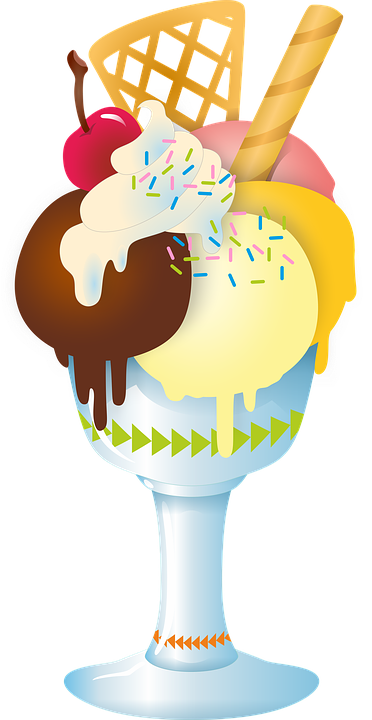
\includegraphics[width=1.61997in,height=3.13542in]{media/image20.png}

\textbf{Sorvete de Azeitona}

O garoto chega na sorveteria e pergunta:

─ Tem sorvete de azeitona?

O vendedor responde:

─ Não.

No dia seguinte:

─ Tem sorvete de azeitona?

─ Não.

No outro dia:

─ Tem sorvete de azeitona?

─ Não.

No outro dia:

─ Tem sorvete de azeitona?

─Tem!

─ Eca!

Domínio Público.

a) Qual é a finalidade desse texto? Comente com os alunos que o gênero
textual anedota é humorístico e tem por objetivo provocar o riso no
leitor.

( ) Contar uma história. ( x ) Causar o riso.

b) Releia o trecho a seguir:

\begin{longtable}[]{@{}l@{}}
\toprule
\begin{minipage}[t]{0.97\columnwidth}\raggedright\strut
O garoto chega na sorveteria e pergunta:

─ Tem sorvete de azeitona?

O vendedor responde:

─ Não.\strut
\end{minipage}\tabularnewline
\bottomrule
\end{longtable}

\begin{itemize}
\item
  Quais são os verbos que introduzem as falas das personagens? Pergunta
  e responde
\end{itemize}

\begin{quote}
\_\_\_\_\_\_\_\_\_\_\_\_\_\_\_\_\_\_\_\_\_\_\_\_\_\_\_\_\_\_\_\_\_\_\_\_\_\_\_\_\_\_\_\_\_\_\_\_\_\_\_\_\_\_\_\_\_\_\_\_\_\_\_\_

\_\_\_\_\_\_\_\_\_\_\_\_\_\_\_\_\_\_\_\_\_\_\_\_\_\_\_\_\_\_\_\_\_\_\_\_\_\_\_\_\_\_\_\_\_\_\_\_\_\_\_\_\_\_\_\_\_\_\_\_\_\_\_\_
\end{quote}

c) Forme dupla com um colega e reescreva o trecho usando o discurso
indireto. Sugestão de resposta: O garoto chega na sorveteria e pergunta
ao vendedor se tem sorvete de azeitona. O vendedor responde que não.

\begin{quote}
\_\_\_\_\_\_\_\_\_\_\_\_\_\_\_\_\_\_\_\_\_\_\_\_\_\_\_\_\_\_\_\_\_\_\_\_\_\_\_\_\_\_\_\_\_\_\_\_\_\_\_\_\_\_\_\_\_\_\_\_\_\_\_\_

\_\_\_\_\_\_\_\_\_\_\_\_\_\_\_\_\_\_\_\_\_\_\_\_\_\_\_\_\_\_\_\_\_\_\_\_\_\_\_\_\_\_\_\_\_\_\_\_\_\_\_\_\_\_\_\_\_\_\_\_\_\_\_\_

\_\_\_\_\_\_\_\_\_\_\_\_\_\_\_\_\_\_\_\_\_\_\_\_\_\_\_\_\_\_\_\_\_\_\_\_\_\_\_\_\_\_\_\_\_\_\_\_\_\_\_\_\_\_\_\_\_\_\_\_\_\_\_\_

\_\_\_\_\_\_\_\_\_\_\_\_\_\_\_\_\_\_\_\_\_\_\_\_\_\_\_\_\_\_\_\_\_\_\_\_\_\_\_\_\_\_\_\_\_\_\_\_\_\_\_\_\_\_\_\_\_\_\_\_\_\_\_\_
\end{quote}

\subsection{Treino}\label{treino-5}

\begin{quote}
1. (Fácil) Leia o início da narrativa ``Cinderela''.

\textbf{CINDERELA}

Há muito tempo, aconteceu que a esposa de um rico comerciante adoeceu
gravemente e, sentindo seu fim se aproximar, chamou sua única filha e
disse:

--- Querida filha, continue piedosa e boa menina que Deus a protegerá
sempre. Lá do céu olharei por você, e estarei sempre a seu lado --- mal
acabou de dizer isso, fechou os olhos e morreu.

\textbf{Cinderela}. Disponível em:

www.dominiopublico.gov.br/download/texto/me000589.pdf. Acesso em: 21
fev. 2023.

O trecho ``--- Querida filha, continue piedosa e boa menina que Deus a
protegerá sempre.'' está em discurso

(A) direto, porque é a fala do personagem separada por travessão.

(B) indireto, porque é a fala do personagem por meio do narrador.

(C) direto, porque é a transcrição da fala do próprio narrador do conto.

(D) indireto, porque apresenta a introdução do narrador ``disse''.

Saeb D7 - Relacionar, na compreensão do texto, informações textuais com
conhecimentos de senso comum.

BNCC EF35LP30: Diferenciar discurso indireto e discurso direto,
determinando o efeito de sentido de verbos de enunciação e explicando o
uso de variedades linguísticas no discurso direto, quando for o caso.

(A) Correta. O trecho apresentado é a fala direta da personagem, como se
vê pela separação feita pelos dois pontos e travessão.

(B) Incorreta. O trecho apresenta uma fala direta.

(C) Incorreta. A fala é introduzida pela esposa.

(D) Incorreta. O verbo de elocução é seguido pelos dois-pontos e pelo
travessão, o que mostra uma separação entre o discurso do narrador e a
fala do personagem, caracterizando como discurso direto.

2. Leia a versão do conto popular ``O príncipe-rã ou Henrique de
ferro'', dos Irmãos Grimm.

\textbf{O príncipe-rã ou Henrique de ferro}

{[}\ldots{}{]} No dia seguinte, quando o rei, a rainha e as filhas
estavam jantando, ouviram um barulho estranho: Plaft!\ldots{}
Plaft!\ldots{} alguém estava subindo a escadaria de mármore do
palácio\ldots{} O barulho cessou bem em frente à porta, e alguém chamou:

--- Abra a porta, filha mais nova do rei!

A princesa foi atender e, quando deu com a rã, tornou a fechar a porta
bem depressa e voltou para a mesa. O rei reparou que ela estava
vermelhinha e apavorada.

--- O que foi, filha? Aí fora está algum gigante, querendo pegar você?
{[}\ldots{}{]}

IRMÃOS GRIMM. \textbf{O príncipe-rã ou Henrique de ferro}. Disponível
em:

www.dominiopublico.gov.br/download/texto/me000589.pdf. Acesso em: 21
fev. 2023.

O primeiro discurso direto encontrado no texto anuncia uma fala

(A) da rainha.

(B) da filha mais nova do rei.

(C) da rã.

(D) do rei.

Saeb D7 - Relacionar, na compreensão do texto, informações textuais com
conhecimentos de senso comum.

BNCC EF35LP22: Perceber diálogos em textos narrativos, observando o
efeito de sentido de verbos de enunciação e, se for o caso, o uso de
variedades linguísticas no discurso direto.

(A) Incorreta. Não foi a rainha quem proferiu o discurso direto.

(B) Incorreta. No trecho, a filha mais nova do rei não profere nenhum
discurso direto.

(C) Correta. O discurso direto ``--- Abra a porta, filha mais nova do
rei!'' é dito pela rã.

(D) Incorreta. O discurso em questão não é dito pelo rei.

3. (Difícil) O conto ``O príncipe canário'' foi escrito pelo escritor
Ítalo Calvino e narra a história de uma princesa que é trancada em uma
torre em razão da inveja de sua madrasta. Leia o início da narrativa.

\textbf{O príncipe canário}

Era uma vez um rei que tinha uma filha. A mãe da menina morrera e a
madrasta sentia muito ciúme da enteada; sempre falava mal dela para o
rei.

A moça vivia a se desculpar e a se desesperar; porém, a madrasta tanto
falou e tanto fez que o rei, embora afeiçoado à filha, acabou dando
razão à rainha e decidiu expulsá-la de casa. Contudo, disse que ela
deveria ficar em um lugar no qual se instalasse bem, pois não admitiria
que fosse maltratada. {[}\ldots{}{]}

CALVINO, Ítalo. \textbf{O príncipe canário}. Disponível em:

www.dominiopublico.gov.br/download/texto/me000589.pdf. Acesso em: 21
fev. 2023.

Para narrar o início do conto, foram utilizados os recursos do discurso

\protect\hypertarget{_Hlk127859316}{}{}(A) indireto e de verbos de
elocução, como ``sentia''.

(B) indireto e de verbos de elocução, como ``disse''.

(C) direto e de verbos de elocução, como ``falava''.

(D) direto e de verbos de elocução, como ``admitiria''.

Saeb D18 -- Reconhecer o efeito de sentido decorrente da escolha de uma
determinada palavra ou expressão.

BNCC EF35LP30 - Diferenciar discurso indireto e discurso direto,
determinando o efeito de sentido de verbos de enunciação e explicando o
uso de variedades linguísticas no discurso direto, quando for o caso.

(A) Incorreta. O texto apresenta discurso indireto, mas o verbo
``sentia'' não é um verbo de elocução.

(B) Correta. O começo da narrativa de ``O príncipe canário''
caracteriza-se pela utilização do recurso do discurso indireto, visto
que o próprio narrador reproduz a natureza das falas das personagens,
como ocorre no trecho ``Contudo, disse que ela deveria ficar em um lugar
no qual se instalasse bem (\ldots{})'', no qual há também o uso do verbo
de elocução ``disse''.

(C) Incorreta. Mesmo que a palavra ``falava'' seja um verbo de elocução,
o trecho não apresenta discurso direto.

(D) Incorreta. No trecho do conto, não há discurso direto, e
``admitiria'' não é um verbo de elocução.
\end{quote}

\section{Módulo 7}\label{muxf3dulo-7}

\begin{quote}
Neste módulo, os alunos vão identificar adjetivos em textos e os
substantivos a que se referem, assim como relacionar substantivos e
adjetivos, observando a concordância de gênero e número.
\end{quote}

\subsection{Conteúdo}\label{conteuxfado-6}

\begin{quote}
\textbf{ADJETIVOS}

Provavelmente, você já deve ter notado que tudo que existe no planeta
tem um nome. Imagine a seguinte situação: você está deitado na cama,
olhando para a televisão, e esta televisão provavelmente está na
estante. Você agora deve estar usando um pijama e comendo uma pipoca
para assistir a um filme.

\textbf{Substantivo} é o nome de cada coisa existente. As palavras que
estão destacadas no trecho acima denominam-se substantivos! Existem
diversas formas de classificar um substantivo: por exemplo, uma
\emph{pizza} pode ser doce ou salgada, em relação ao sabor; pelo
tamanho, pode ser grande ou pequena. E também podemos dizer que ele é
barata ou cara, em relação ao preço! Essas características que podemos
dar a um substantivo, chamamos de \textbf{adjetivos}, que são palavras
que modificam o significado do substantivo, acrescentando-lhe noções de
qualidade, natureza, estado etc.

A palavra \textbf{cachorro} é um substantivo que dá nome a um animal
doméstico. Observe quantas características o cachorro pode ter:

https://pixabay.com/pt/photos/filhote-de-cachorro-cachorro-1903313/

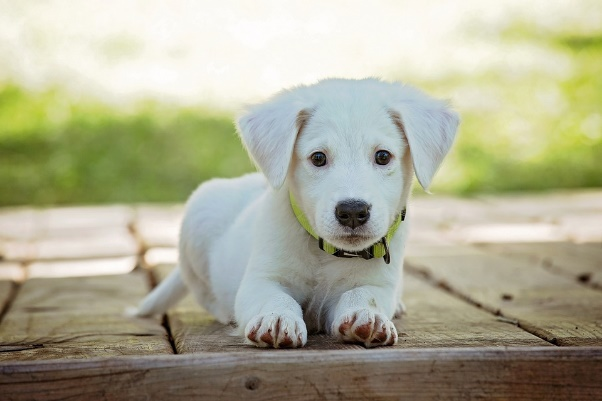
\includegraphics[width=2.71875in,height=1.81239in]{media/image21.jpeg}

\textbf{branco / filhote / fofo / amigo}

Agora, veja alguns exemplos de características que podemos dar a um
\textbf{sanduíche}:

https://pixabay.com/pt/photos/hamburger-hamb\%c3\%barguer-churrasco-1238246/

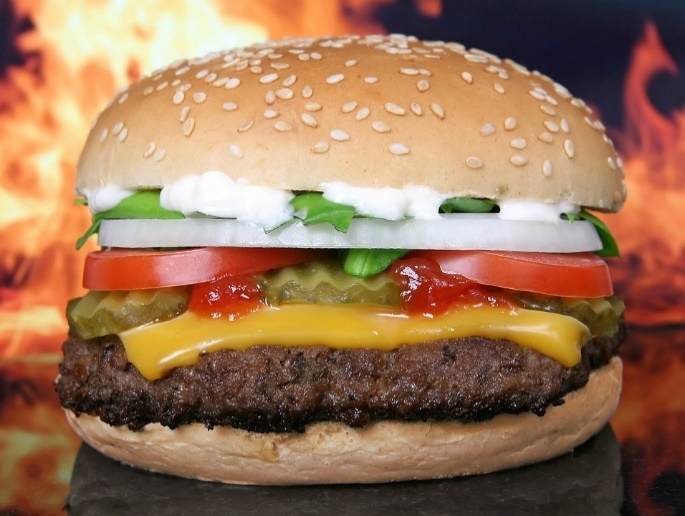
\includegraphics[width=3.11183in,height=2.34375in]{media/image22.jpeg}

\textbf{Saboroso / quente / grande / salgado}
\end{quote}

\subsection{Atividades}\label{atividades-6}

\begin{quote}
\textbf{Carta de leitor} é uma carta destinada a veículos de comunicação
da mídia impressa ou digital com o objetivo de manifestar impressões,
opiniões, sugestões em relação a fatos veiculados ou não.

Caso julgue pertinente, providencie exemplos de cartas de leitores,
trazendo para a sala de aula jornais e revistas impressos abertos nessa
seção e apresente aos alunos.
\end{quote}

\subsubsection{1. }\label{section-57}

\begin{quote}
Leia uma carta de um leitor publicada em uma revista especializada em
divulgação científica, dirigida aos jovens.

\textbf{Lagartos}

Olá, pessoal da CHC! \protect\hypertarget{_Hlk127887653}{}{}Ficamos
muito impressionados com o texto: ``\emph{Por que o lagarto balança
tanto a cabeça?}'', publicado na CHC 244, que fala sobre o
lagarto-cinzento. Ele usa a cabeça para se comunicar com outros da mesma
espécie. Eles se comportam assim para informar se são machos ou fêmeas.
Eles vivem num ambiente natural como, rochas, embaixo d'água, da terra,
e sobre árvores. Gostamos muito do texto e ficaríamos bem felizes se
nossa cartinha fosse publicada. Um grande abraço.

Alunos do 3º ano da Escola Municipal Professor João Oliveira Lima.
Pontal, Quixeré-Ce.

CHC. Lagartos. Fala Aqui!, Ciência Hoje das Crianças, ed. 244.
Disponível em:
https://chc.org.br/artigo/fala-aqui/\#:\textasciitilde{}:text=Ficamos\%20muito\%20impressionados\%20com\%20o,se\%20s\%C3\%A3o\%20machos\%20ou\%20f\%C3\%AAmeas..
Acesso em: 21 fev. 2023.

a) Qual é o assunto dessa carta? Os alunos ficaram muito impressionados
com o texto ``Por que o lagarto balança tanto a cabeça?'', publicado na
CHC 244, que fala sobre o lagarto-cinzento.

\protect\hypertarget{_Hlk127887290}{}{}\_\_\_\_\_\_\_\_\_\_\_\_\_\_\_\_\_\_\_\_\_\_\_\_\_\_\_\_\_\_\_\_\_\_\_\_\_\_\_\_\_\_\_\_\_\_\_\_\_\_\_\_\_\_\_\_\_\_\_\_\_\_\_\_

\_\_\_\_\_\_\_\_\_\_\_\_\_\_\_\_\_\_\_\_\_\_\_\_\_\_\_\_\_\_\_\_\_\_\_\_\_\_\_\_\_\_\_\_\_\_\_\_\_\_\_\_\_\_\_\_\_\_\_\_\_\_\_\_

\_\_\_\_\_\_\_\_\_\_\_\_\_\_\_\_\_\_\_\_\_\_\_\_\_\_\_\_\_\_\_\_\_\_\_\_\_\_\_\_\_\_\_\_\_\_\_\_\_\_\_\_\_\_\_\_\_\_\_\_\_\_\_\_

\_\_\_\_\_\_\_\_\_\_\_\_\_\_\_\_\_\_\_\_\_\_\_\_\_\_\_\_\_\_\_\_\_\_\_\_\_\_\_\_\_\_\_\_\_\_\_\_\_\_\_\_\_\_\_\_\_\_\_\_\_\_\_\_
\end{quote}

\begin{enumerate}
\def\labelenumi{\alph{enumi})}
\item
  A quem a carta foi destinada? Ao pessoal da revista CHC.
\end{enumerate}

\begin{quote}
\_\_\_\_\_\_\_\_\_\_\_\_\_\_\_\_\_\_\_\_\_\_\_\_\_\_\_\_\_\_\_\_\_\_\_\_\_\_\_\_\_\_\_\_\_\_\_\_\_\_\_\_\_\_\_\_\_\_\_\_\_\_\_\_

\_\_\_\_\_\_\_\_\_\_\_\_\_\_\_\_\_\_\_\_\_\_\_\_\_\_\_\_\_\_\_\_\_\_\_\_\_\_\_\_\_\_\_\_\_\_\_\_\_\_\_\_\_\_\_\_\_\_\_\_\_\_\_\_
\end{quote}

\begin{enumerate}
\def\labelenumi{\alph{enumi})}
\item
  Quem é o remetente da carta? Alunos do 3º ano da Escola Municipal
  Professor João Oliveira Lima. Pontal, Quixeré-Ce.
\end{enumerate}

\begin{quote}
\_\_\_\_\_\_\_\_\_\_\_\_\_\_\_\_\_\_\_\_\_\_\_\_\_\_\_\_\_\_\_\_\_\_\_\_\_\_\_\_\_\_\_\_\_\_\_\_\_\_\_\_\_\_\_\_\_\_\_\_\_\_\_\_

\_\_\_\_\_\_\_\_\_\_\_\_\_\_\_\_\_\_\_\_\_\_\_\_\_\_\_\_\_\_\_\_\_\_\_\_\_\_\_\_\_\_\_\_\_\_\_\_\_\_\_\_\_\_\_\_\_\_\_\_\_\_\_\_

\_\_\_\_\_\_\_\_\_\_\_\_\_\_\_\_\_\_\_\_\_\_\_\_\_\_\_\_\_\_\_\_\_\_\_\_\_\_\_\_\_\_\_\_\_\_\_\_\_\_\_\_\_\_\_\_\_\_\_\_\_\_\_\_
\end{quote}

\begin{enumerate}
\def\labelenumi{\alph{enumi})}
\item
  Circule o trecho da carta em que os leitores expressam sua opinião. Os
  alunos deve circular o trecho: Ficamos muito impressionados com o
  texto: ``\emph{Por que o lagarto balança tanto a cabeça?}'', publicado
  na CHC 244, que fala sobre o lagarto-cinzento.
\item
  Do trecho que você copiou, qual palavra o leitor usa para caracterizar
  o tema? Impressionados
\end{enumerate}

\begin{quote}
\_\_\_\_\_\_\_\_\_\_\_\_\_\_\_\_\_\_\_\_\_\_\_\_\_\_\_\_\_\_\_\_\_\_\_\_\_\_\_\_\_\_\_\_\_\_\_\_\_\_\_\_\_\_\_\_\_\_\_\_\_\_\_\_
\end{quote}

\begin{enumerate}
\def\labelenumi{\alph{enumi})}
\item
  Que outro adjetivo poderia substituir impressionados no texto, sem
  alterar o sentido? Marque a alternativa correta.
\end{enumerate}

\begin{quote}
( x ) maravilhados

( ) chateados

( ) decepcionados
\end{quote}

\subsubsection{2. }\label{section-58}

Leia um trecho do poema ``Meiguice'', de Adelina Lopes Vieira.

\begin{quote}
Inserir imagem ao lado do texto:
\url{https://pixabay.com/pt/illustrations/gato-filhote-de-cachorro-7347316/}

Destacar de verde as palavras do texto


\includegraphics[width=3.41667in,height=3.07500in]{media/image23.png}

\textbf{Meiguice}

{[}...{]}

Deram à linda Clarisse

uma gatinha mimosa,

tão branca, tão carinhosa,

tão engraçada, tão mansa

que a encantadora criança

por nome lhe pôs --- Meiguice.

{[}...{]}

VIEIRA, Adelina Lopes. \textbf{Meiguice}. Disponível em:
\url{http://www.dominiopublico.gov.br/download/texto/wk000075.pdf}.
Acesso em: 21 fev. 2023.

a) Que nome Clarisse deu à gatinha que ganhou? Meiguice

\_\_\_\_\_\_\_\_\_\_\_\_\_\_\_\_\_\_\_\_\_\_\_\_\_\_\_\_\_\_\_\_\_\_\_\_\_\_\_\_\_\_\_\_\_\_\_\_\_\_\_\_\_\_\_\_\_\_\_\_\_\_\_\_

b) Por que Clarisse deu o nome de Meiguice à sua gatinha? Porque ela era
uma gatinha mimosa, tão branca, tão carinhosa, tão engraçada, tão mansa.

\_\_\_\_\_\_\_\_\_\_\_\_\_\_\_\_\_\_\_\_\_\_\_\_\_\_\_\_\_\_\_\_\_\_\_\_\_\_\_\_\_\_\_\_\_\_\_\_\_\_\_\_\_\_\_\_\_\_\_\_\_\_\_\_

\_\_\_\_\_\_\_\_\_\_\_\_\_\_\_\_\_\_\_\_\_\_\_\_\_\_\_\_\_\_\_\_\_\_\_\_\_\_\_\_\_\_\_\_\_\_\_\_\_\_\_\_\_\_\_\_\_\_\_\_\_\_\_\_

\_\_\_\_\_\_\_\_\_\_\_\_\_\_\_\_\_\_\_\_\_\_\_\_\_\_\_\_\_\_\_\_\_\_\_\_\_\_\_\_\_\_\_\_\_\_\_\_\_\_\_\_\_\_\_\_\_\_\_\_\_\_\_\_

\_\_\_\_\_\_\_\_\_\_\_\_\_\_\_\_\_\_\_\_\_\_\_\_\_\_\_\_\_\_\_\_\_\_\_\_\_\_\_\_\_\_\_\_\_\_\_\_\_\_\_\_\_\_\_\_\_\_\_\_\_\_\_\_

c) Pinte de verde todos os adjetivos do texto. Gabarito marcado no
texto.
\end{quote}

\subsubsection{3. }\label{section-59}

\begin{quote}
Relacione os substantivos aos adjetivos que podem caracterizá-los.

Fazer gabarito em magenta.

ruas quentinho

sapato peludo

bolo esburacadas

cachorro alto

vestido ruivo

cabelo curto
\end{quote}

\subsection{Treino}\label{treino-6}

\begin{quote}
1. (Fácil) Leia um trecho de um conto popular.

\textbf{A guardadora de patos}

Era uma vez uma velha, muito velhinha, toda corcovada, que vivia com o
seu bando de patos num lugar deserto, no meio das montanhas, onde tinha
uma linda casinha. o sítio estava cercado de uma grande floresta onde a
velha ia todas as manhãs, servindo-se de uma muleta para poder andar.
trabalhava ali horas e horas com uma força extraordinária para a sua
idade; cortava a erva para os patos, que muito gostavam disso
{[}\ldots{}{]}.

IRMÃOS GRIMM. Contos dos Irmãos Grimm. Rio de Janeiro: Livraria Garnier,
1932, p. 7. Disponível em: https://digital.bbm.usp.br/handle/bbm/7812.
Acesso em: 22 fev. 2023.

Glossário:

\textbf{Corcovada}: corcunda.

Pela leitura do texto, uma das palavras que caracterizam a guardadora de
patos é

(A) ``deserto''.

(B) ``velhinha''.

(C) ``linda''.

(D) ``grande''.

Saeb D5 - Inferir o sentido de uma palavra ou expressão a partir do
contexto imediato.

BNCC EF03LP09 - Identificar, em textos, adjetivos e sua função de
atribuição de propriedades aos substantivos.

(A) Incorreta. A palavra ``deserto'' caracteriza o espaço em que se
passa a narrativa.

(B) Correta. ``Velhinha'' é uma das palavras que caracterizam a
guardadora de patos, a personagem principal da história.

(C) Incorreta. ``Linda'' caracteriza a casa da personagem.

(D) Incorreta. ``Grande'' caracteriza o espaço da narrativa.

2. (Médio) Leia a carta ao leitor a seguir.

\textbf{Fama de guloso}

Somos alunos do 5º ano. Lemos um texto sobre a fama de D. João VI de ser
guloso. Gostamos muito dessa curiosidade e compreendemos por que os
artistas o retrataram gordinho nos quadros e nos livros de história.
Imaginamos as festas que o rei promovia naquela época {[}\ldots{}{]}

CIÊNCIA HOJE DAS CRIANÇAS. \textbf{Fama de guloso}. Disponível em:
http://chc.org.br/artigo/fala-aqui-303/. Acesso em: 22 fev. 2023.

Uma das características de D. João VI, citada no trecho, era

(A) ser ``gordinho'', palavra que é um adjetivo.

(B) ser ``guloso'', palavra que é um substantivo.

(C) a ``curiosidade'', palavra que é um adjetivo.

(D) ser ``importante'', palavra que é um substantivo.

Saeb D6 - Utilizar informações oferecidas por um glossário, verbete de
dicionário ou texto informativo na compreensão ou interpretação do
texto.

BNCC EF03LP23 - Analisar o uso de adjetivos em cartas dirigidas a
veículos da mídia impressa ou digital (cartas do leitor ou de reclamação
a jornais ou revistas), digitais ou impressas.

(A) Correta. Conforme o trecho, D. João IV era ``gordinho'', que é um
adjetivo.

(B) Incorreta. A palavra ``guloso'' é um adjetivo.

(C) Incorreta. A palavra ``curiosidade'' é substantivo.

(D) Incorreta. A palavra é um adjetivo.

3. (Difícil) Leia a carta de leitor a seguir.

\textbf{Cabeça de jacaré}

Eu li a matéria sobre jacarés e crocodilos na CHC 224. Achei legal!
{[}\ldots{}{]} Como vocês sabem que um crânio de jacaré é mais longo que
de um crocodilo? {[}\ldots{}{]}

Oi, Pedro! Quem dá as informações para os textos da CHC são cientistas.
Cada um é especializado em uma área. O texto que você leu veio de um
especialista em crocodilos e jacarés. Até a próxima!

FALA AQUI, Ciência Hoje das Crianças. Disponível em:
\url{http://chc.org.br/artigo/fala-aqui/}. Acesso em: 22 fev. 2023.

A revista CHC usou o adjetivo ``especializados'' ao responder à carta do
leitor. Essa palavra foi utilizada para

(A) falar ao leitor em relação às pesquisas com crocodilos.

(B) explicar ao leitor como são os jacarés.

(C) garantir ao leitor que a informação era confiável.

(D) dizer ao leitor como ele pode conseguir a informação.

Saeb D6 - Utilizar informações oferecidas por um glossário, verbete de
dicionário ou texto informativo na compreensão ou interpretação do
texto.

BNCC EF03LP23 - Analisar o uso de adjetivos em cartas dirigidas a
veículos da mídia impressa ou digital (cartas do leitor ou de reclamação
a jornais ou revistas), digitais ou impressas.

(A) Incorreta. Utilizou-se o adjetivo para falar do cientista, e não da
pesquisa.

(B) Incorreta. Usou-se o adjetivo para caracterizar a opinião dos
cientistas.

(C) Correta. A CHC usa o adjetivo ``especializados'' para mencionar os
cientistas que escrevem as matérias da revista, garantindo que, como
eles são especialistas, é possível confiar na informação apresentada.

(D) Incorreta. Já se deu a informação, a carta ao leitor explicou a
forma de como ela foi alcançada.
\end{quote}

\section{Módulo 8}\label{muxf3dulo-8}

\begin{quote}
Neste módulo, espera-se que os alunos leiam e compreendam o texto,
identifiquem e localizem informações no texto e façam distinção entre
fatos e opiniões em textos.
\end{quote}

\subsection{Conteúdo}\label{conteuxfado-7}

\begin{quote}
https://pixabay.com/pt/illustrations/coment\%c3\%a1rios-relat\%c3\%b3rio-de-volta-2990424/


\includegraphics[width=3.98294in,height=2.65514in]{media/image24.jpeg}

\textbf{Fato ou opinião?}

\textbf{Fato} é algo que ocorreu e pode ser comprovado de algum modo,
por meio de determinado documento, números, vídeo ou registro. Observe o
exemplo:
\end{quote}

\begin{longtable}[]{@{}l@{}}
\toprule
\begin{minipage}[t]{0.97\columnwidth}\raggedright\strut
\begin{quote}
Há mais alunos matriculados em escolas públicas de Fortaleza - CE.
\end{quote}\strut
\end{minipage}\tabularnewline
\bottomrule
\end{longtable}

\begin{quote}
A informação consiste em um fato, uma vez que há registros dos casos e,
por meio deles, é possível fazer uma afirmação.

\textbf{Opinião} consiste em uma interpretação do fato, isto é, uma
forma pessoal de olhar o fato. Essa opinião pode ser diferente de pessoa
para pessoa a depender de muitos fatores. Veja o exemplo:
\end{quote}

\begin{longtable}[]{@{}l@{}}
\toprule
\begin{minipage}[t]{0.97\columnwidth}\raggedright\strut
\begin{quote}
Se aquela moça fosse mais alta, poderia ser modelo.
\end{quote}\strut
\end{minipage}\tabularnewline
\bottomrule
\end{longtable}

\begin{quote}
Leia o início de uma notícia para entender melhor o que é fato e o que é
opinião.

\textbf{https://chc.org.br/fofos-preguicosos-e-comiloes/}

\textbf{Fofos, preguiçosos e comilões}

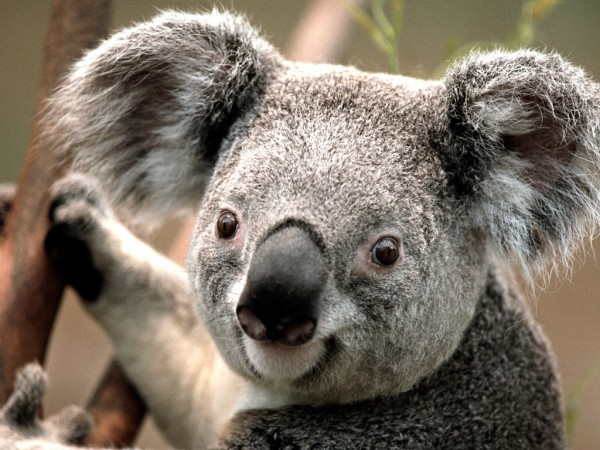
\includegraphics[width=3.61389in,height=2.71042in]{media/image25.jpeg}

Sua aparência engana: apesar de lembrarem ursos de pelúcia, os coalas
são parentes dos cangurus, gambás e outros animais conhecidos
como~marsupiais. Encontrados na Austrália, esses mamíferos passam o dia
inteiro deitados em árvores, comendo folhas e dormindo. Que vida boa,
não é? {[}...{]}

FOFOS, preguiçosos e comilões. CHC.

Disponível em: \url{https://chc.org.br/fofos-preguicosos-e-comiloes/}.
Acesso em: 22 fev. 2023.

Note que o que está em verde apresenta um fato, uma afirmação, uma
certeza. O que está em roxo é uma opinião, pois não se sabe com certeza
se os coalas têm uma vida boa.
\end{quote}

\subsection{Atividades}\label{atividades-7}

\subsubsection{1. }\label{section-60}

\begin{quote}
O ECA é o Estatuto da Criança e do Adolescente que tem como finalidade
proteger e garantir o direito dos jovens. Em 2019, o ECA completou 29
anos desde sua criação.

\textbf{29 anos do ECA}


\includegraphics[width=5.90556in,height=2.30417in]{media/image26.jpeg}

16/07/2019~

No dia 13 de julho, o~Estatuto~da Criança e do Adolescente, o ECA,
completou mais um ano. E como estamos falando de aniversário, é
importante refletir sobre o que realmente se pode comemorar. Como quase
todo mundo já sabe, apesar do apelido engraçado, o ECA é coisa muito
séria. Trata-se do conjunto de normas criadas para garantir direitos e
proteger a criança e o adolescente contra a violência, o trabalho
infantil, a discriminação ou preconceito de qualquer tipo, humilhações
ou crueldades.

Nestes 29 anos, muita coisa boa aconteceu. Houve redução da mortalidade
infantil por crimes, a previsão do amplo acesso ao ensino fundamental, a
criação do plano nacional de educação e a implantação de testes
obrigatórios para recém-nascidos.

\protect\hypertarget{_Hlk128033654}{}{}Além disso, o~Estatuto~sofreu
alterações com o objetivo fazer cumprir o que nele está escrito. Foi
criado o Cadastro Nacional de Pessoas Desaparecidas, a idade mínima para
que a criança possa viajar desacompanhada dos pais passou para 16 anos
{[}...{]}.

Na hora de celebrar uma~legislação~tão importante, não se pode esquecer
os desafios que ainda permanecem. Por isso, é preciso conhecer bem o ECA
e entendê-lo, para defendê-lo!

PLENARINHO. 29 anos do ECA. Disponível em:
https://plenarinho.leg.br/index.php/2019/07/29-anos-eca/. Acesso em: 23
fev. 2023.

a) Segundo informações do texto, o que é o ECA? É o conjunto de normas
criadas para garantir direitos e proteger a criança e o adolescente
contra a violência, o trabalho infantil, a discriminação ou preconceito
de qualquer tipo, humilhações ou crueldades.

\_\_\_\_\_\_\_\_\_\_\_\_\_\_\_\_\_\_\_\_\_\_\_\_\_\_\_\_\_\_\_\_\_\_\_\_\_\_\_\_\_\_\_\_\_\_\_\_\_\_\_\_\_\_\_\_\_\_\_\_\_\_\_\_

\_\_\_\_\_\_\_\_\_\_\_\_\_\_\_\_\_\_\_\_\_\_\_\_\_\_\_\_\_\_\_\_\_\_\_\_\_\_\_\_\_\_\_\_\_\_\_\_\_\_\_\_\_\_\_\_\_\_\_\_\_\_\_\_

\_\_\_\_\_\_\_\_\_\_\_\_\_\_\_\_\_\_\_\_\_\_\_\_\_\_\_\_\_\_\_\_\_\_\_\_\_\_\_\_\_\_\_\_\_\_\_\_\_\_\_\_\_\_\_\_\_\_\_\_\_\_\_\_

\_\_\_\_\_\_\_\_\_\_\_\_\_\_\_\_\_\_\_\_\_\_\_\_\_\_\_\_\_\_\_\_\_\_\_\_\_\_\_\_\_\_\_\_\_\_\_\_\_\_\_\_\_\_\_\_\_\_\_\_\_\_\_\_

b) Qual foi a data de publicação dessa notícia? A data foi 16/07/2019~

\_\_\_\_\_\_\_\_\_\_\_\_\_\_\_\_\_\_\_\_\_\_\_\_\_\_\_\_\_\_\_\_\_\_\_\_\_\_\_\_\_\_\_\_\_\_\_\_\_\_\_\_\_\_\_\_\_\_\_\_\_\_\_\_

\_\_\_\_\_\_\_\_\_\_\_\_\_\_\_\_\_\_\_\_\_\_\_\_\_\_\_\_\_\_\_\_\_\_\_\_\_\_\_\_\_\_\_\_\_\_\_\_\_\_\_\_\_\_\_\_\_\_\_\_\_\_\_\_

c) Em que ano o ECA completou 29 anos? 2019

\_\_\_\_\_\_\_\_\_\_\_\_\_\_\_\_\_\_\_\_\_\_\_\_\_\_\_\_\_\_\_\_\_\_\_\_\_\_\_\_\_\_\_\_\_\_\_\_\_\_\_\_\_\_\_\_\_\_\_\_\_\_\_\_

\_\_\_\_\_\_\_\_\_\_\_\_\_\_\_\_\_\_\_\_\_\_\_\_\_\_\_\_\_\_\_\_\_\_\_\_\_\_\_\_\_\_\_\_\_\_\_\_\_\_\_\_\_\_\_\_\_\_\_\_\_\_\_\_

d) Quais foram as coisas boas que aconteceram nesses 29 anos de ECA?
Houve redução da mortalidade infantil por crimes, a previsão do amplo
acesso ao ensino fundamental, a criação do plano nacional de educação e
a implantação de testes obrigatórios para recém-nascidos.

\_\_\_\_\_\_\_\_\_\_\_\_\_\_\_\_\_\_\_\_\_\_\_\_\_\_\_\_\_\_\_\_\_\_\_\_\_\_\_\_\_\_\_\_\_\_\_\_\_\_\_\_\_\_\_\_\_\_\_\_\_\_\_\_

\_\_\_\_\_\_\_\_\_\_\_\_\_\_\_\_\_\_\_\_\_\_\_\_\_\_\_\_\_\_\_\_\_\_\_\_\_\_\_\_\_\_\_\_\_\_\_\_\_\_\_\_\_\_\_\_\_\_\_\_\_\_\_\_

\protect\hypertarget{_Hlk128040463}{}{}\_\_\_\_\_\_\_\_\_\_\_\_\_\_\_\_\_\_\_\_\_\_\_\_\_\_\_\_\_\_\_\_\_\_\_\_\_\_\_\_\_\_\_\_\_\_\_\_\_\_\_\_\_\_\_\_\_\_\_\_\_\_\_\_

\_\_\_\_\_\_\_\_\_\_\_\_\_\_\_\_\_\_\_\_\_\_\_\_\_\_\_\_\_\_\_\_\_\_\_\_\_\_\_\_\_\_\_\_\_\_\_\_\_\_\_\_\_\_\_\_\_\_\_\_\_\_\_\_

\_\_\_\_\_\_\_\_\_\_\_\_\_\_\_\_\_\_\_\_\_\_\_\_\_\_\_\_\_\_\_\_\_\_\_\_\_\_\_\_\_\_\_\_\_\_\_\_\_\_\_\_\_\_\_\_\_\_\_\_\_\_\_\_
\end{quote}

\begin{enumerate}
\def\labelenumi{\alph{enumi})}
\item
  Segundo o texto, o que é necessário para defender o ECA? É preciso
  conhecer bem e entendê-lo.
\end{enumerate}

\begin{quote}
\_\_\_\_\_\_\_\_\_\_\_\_\_\_\_\_\_\_\_\_\_\_\_\_\_\_\_\_\_\_\_\_\_\_\_\_\_\_\_\_\_\_\_\_\_\_\_\_\_\_\_\_\_\_\_\_\_\_\_\_\_\_\_\_

\_\_\_\_\_\_\_\_\_\_\_\_\_\_\_\_\_\_\_\_\_\_\_\_\_\_\_\_\_\_\_\_\_\_\_\_\_\_\_\_\_\_\_\_\_\_\_\_\_\_\_\_\_\_\_\_\_\_\_\_\_\_\_\_

\_\_\_\_\_\_\_\_\_\_\_\_\_\_\_\_\_\_\_\_\_\_\_\_\_\_\_\_\_\_\_\_\_\_\_\_\_\_\_\_\_\_\_\_\_\_\_\_\_\_\_\_\_\_\_\_\_\_\_\_\_\_\_\_

g) Numere as frases a seguir de acordo com a ordem das informações do
texto.

( 3 ) Nestes 29 anos, muita coisa boa aconteceu.

( 1 ) No dia 13 de julho, o~Estatuto~da Criança e do Adolescente, o ECA,
completou mais um ano.

( 4 ) Além disso, o~Estatuto~sofreu alterações com o objetivo fazer
cumprir o que nele está escrito.

( 2 ) Como quase todo mundo já sabe, apesar do apelido engraçado, o ECA
é coisa muito séria.

( 5 ) Por isso, é preciso conhecer bem o ECA e entendê-lo, para
defendê-lo!
\end{quote}

\subsubsection{2. }\label{section-61}

\begin{quote}
Releia este trecho do texto.
\end{quote}

\begin{longtable}[]{@{}l@{}}
\toprule
\begin{minipage}[t]{0.97\columnwidth}\raggedright\strut
Além disso, o~Estatuto~sofreu alterações com o objetivo fazer cumprir o
que nele está escrito. Foi criado o Cadastro Nacional de Pessoas
Desaparecidas, a idade mínima para que a criança possa viajar
desacompanhada dos pais passou para 16 anos {[}...{]}.

Na hora de celebrar uma~legislação~tão importante, não se pode esquecer
os desafios que ainda permanecem. Por isso, é preciso conhecer bem o ECA
e entendê-lo, para defendê-lo!\strut
\end{minipage}\tabularnewline
\bottomrule
\end{longtable}

\begin{quote}
a) Escreva o trecho que expressa:

Auxilie os alunos a distinguir fato de opinião, pois esse assunto é um
relativamente complexo para eles, mas é\\
fundamental que, gradativamente, eles se\\
habituem a realizar esse tipo de análise.
\end{quote}

\begin{itemize}
\item
  O \textbf{fato} que foi informado: o~Estatuto~sofreu alterações com o
  objetivo fazer cumprir o que nele está escrito.
\end{itemize}

\begin{quote}
\_\_\_\_\_\_\_\_\_\_\_\_\_\_\_\_\_\_\_\_\_\_\_\_\_\_\_\_\_\_\_\_\_\_\_\_\_\_\_\_\_\_\_\_\_\_\_\_\_\_\_\_\_\_\_\_\_\_\_\_\_\_\_\_

\_\_\_\_\_\_\_\_\_\_\_\_\_\_\_\_\_\_\_\_\_\_\_\_\_\_\_\_\_\_\_\_\_\_\_\_\_\_\_\_\_\_\_\_\_\_\_\_\_\_\_\_\_\_\_\_\_\_\_\_\_\_\_\_

\_\_\_\_\_\_\_\_\_\_\_\_\_\_\_\_\_\_\_\_\_\_\_\_\_\_\_\_\_\_\_\_\_\_\_\_\_\_\_\_\_\_\_\_\_\_\_\_\_\_\_\_\_\_\_\_\_\_\_\_\_\_\_\_
\end{quote}

\begin{itemize}
\item
  A \textbf{opinião} dos autores do texto: Na hora de celebrar uma
  legislação tão importante, não se pode esquecer os desafios que ainda
  permanecem.
\end{itemize}

\begin{quote}
\_\_\_\_\_\_\_\_\_\_\_\_\_\_\_\_\_\_\_\_\_\_\_\_\_\_\_\_\_\_\_\_\_\_\_\_\_\_\_\_\_\_\_\_\_\_\_\_\_\_\_\_\_\_\_\_\_\_\_\_\_\_\_\_

\_\_\_\_\_\_\_\_\_\_\_\_\_\_\_\_\_\_\_\_\_\_\_\_\_\_\_\_\_\_\_\_\_\_\_\_\_\_\_\_\_\_\_\_\_\_\_\_\_\_\_\_\_\_\_\_\_\_\_\_\_\_\_\_

\_\_\_\_\_\_\_\_\_\_\_\_\_\_\_\_\_\_\_\_\_\_\_\_\_\_\_\_\_\_\_\_\_\_\_\_\_\_\_\_\_\_\_\_\_\_\_\_\_\_\_\_\_\_\_\_\_\_\_\_\_\_\_\_
\end{quote}

\begin{itemize}
\item
  O \textbf{motivo} da opinião dos autores do texto: Por isso, é preciso
  conhecer bem o ECA e entendê-lo, para defendê-lo!
\end{itemize}

\begin{quote}
\_\_\_\_\_\_\_\_\_\_\_\_\_\_\_\_\_\_\_\_\_\_\_\_\_\_\_\_\_\_\_\_\_\_\_\_\_\_\_\_\_\_\_\_\_\_\_\_\_\_\_\_\_\_\_\_\_\_\_\_\_\_\_\_

\_\_\_\_\_\_\_\_\_\_\_\_\_\_\_\_\_\_\_\_\_\_\_\_\_\_\_\_\_\_\_\_\_\_\_\_\_\_\_\_\_\_\_\_\_\_\_\_\_\_\_\_\_\_\_\_\_\_\_\_\_\_\_\_

\_\_\_\_\_\_\_\_\_\_\_\_\_\_\_\_\_\_\_\_\_\_\_\_\_\_\_\_\_\_\_\_\_\_\_\_\_\_\_\_\_\_\_\_\_\_\_\_\_\_\_\_\_\_\_\_\_\_\_\_\_\_\_\_
\end{quote}

\subsubsection{3. }\label{section-62}

Leia mais um trecho de texto relacionado ao ECA.

\begin{quote}
Se julgar pertinente, após a leitura do trecho, comente com os alunos
que, antes de o Estatuto da Criança e do Adolescente (ECA) ser
promulgado, era comum ver crianças trabalhando em vez de estudar ou
brincar.

https://pixabay.com/pt/illustrations/diversidade-igualdade-crian\%c3\%a7as-5392891/

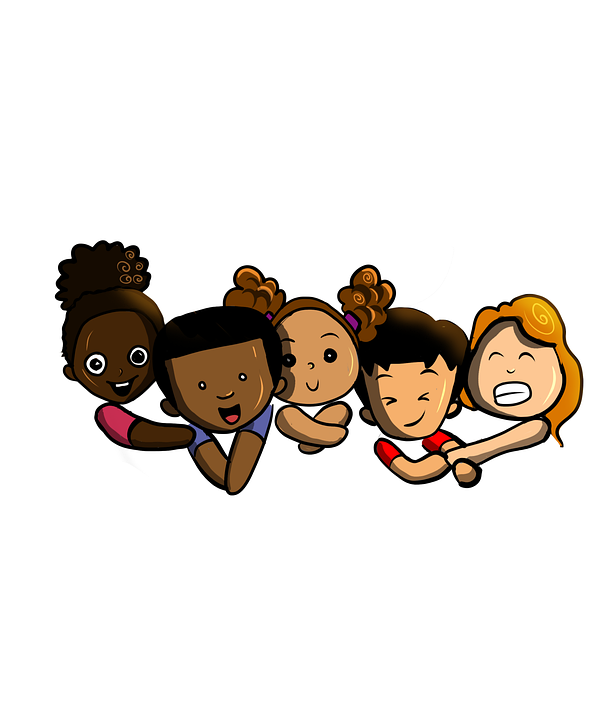
\includegraphics[width=2.70833in,height=3.25006in]{media/image27.png}

Inserir cores, conforme modelo.

{[}...{]}

A família, base da sociedade, é lugar onde os vínculos afetivos são
fortalecidos. Crianças são seres com diversas particularidades em fase
de desenvolvimento, por isso elas têm de brincar, estudar, tem que ser
amadas e devem se expressar. Esse é o período de ser protegida dentro
dessa condição de pessoa em desenvolvimento e que tem prioridade
absoluta. O estatuto valoriza esses vínculos e elos que são fundamentais
para o florescimento humano.

{[}...{]}

Disponível em:
\url{https://www.novaserrana.mg.gov.br/portal/noticias/0/3/3550/estatuto-da-crianca-e-do-adolescente-completa-30-anos}.
Acesso em: 23 fev. 2023.

a) O que é família, segundo informações do texto? A família, base da
sociedade, é lugar onde os vínculos afetivos são fortalecidos

\_\_\_\_\_\_\_\_\_\_\_\_\_\_\_\_\_\_\_\_\_\_\_\_\_\_\_\_\_\_\_\_\_\_\_\_\_\_\_\_\_\_\_\_\_\_\_\_\_\_\_\_\_\_\_\_\_\_\_\_\_\_\_\_

\_\_\_\_\_\_\_\_\_\_\_\_\_\_\_\_\_\_\_\_\_\_\_\_\_\_\_\_\_\_\_\_\_\_\_\_\_\_\_\_\_\_\_\_\_\_\_\_\_\_\_\_\_\_\_\_\_\_\_\_\_\_\_\_

\_\_\_\_\_\_\_\_\_\_\_\_\_\_\_\_\_\_\_\_\_\_\_\_\_\_\_\_\_\_\_\_\_\_\_\_\_\_\_\_\_\_\_\_\_\_\_\_\_\_\_\_\_\_\_\_\_\_\_\_\_\_\_\_

b) Conforme informações do trecho, as crianças são seres em fase de
desenvolvimento. Quais são os direitos delas?

\_\_\_\_\_\_\_\_\_\_\_\_\_\_\_\_\_\_\_\_\_\_\_\_\_\_\_\_\_\_\_\_\_\_\_\_\_\_\_\_\_\_\_\_\_\_\_\_\_\_\_\_\_\_\_\_\_\_\_\_\_\_\_\_

\_\_\_\_\_\_\_\_\_\_\_\_\_\_\_\_\_\_\_\_\_\_\_\_\_\_\_\_\_\_\_\_\_\_\_\_\_\_\_\_\_\_\_\_\_\_\_\_\_\_\_\_\_\_\_\_\_\_\_\_\_\_\_\_

\_\_\_\_\_\_\_\_\_\_\_\_\_\_\_\_\_\_\_\_\_\_\_\_\_\_\_\_\_\_\_\_\_\_\_\_\_\_\_\_\_\_\_\_\_\_\_\_\_\_\_\_\_\_\_\_\_\_\_\_\_\_\_\_

c) Dos trechos destacados, qual deles expressa um fato? Qual deles
expressa uma opinião?

O trecho destacado em verde expressa um fato. O trecho destacado em azul
expressa uma opinião.

\_\_\_\_\_\_\_\_\_\_\_\_\_\_\_\_\_\_\_\_\_\_\_\_\_\_\_\_\_\_\_\_\_\_\_\_\_\_\_\_\_\_\_\_\_\_\_\_\_\_\_\_\_\_\_\_\_\_\_\_\_\_\_\_

\_\_\_\_\_\_\_\_\_\_\_\_\_\_\_\_\_\_\_\_\_\_\_\_\_\_\_\_\_\_\_\_\_\_\_\_\_\_\_\_\_\_\_\_\_\_\_\_\_\_\_\_\_\_\_\_\_\_\_\_\_\_\_\_

\_\_\_\_\_\_\_\_\_\_\_\_\_\_\_\_\_\_\_\_\_\_\_\_\_\_\_\_\_\_\_\_\_\_\_\_\_\_\_\_\_\_\_\_\_\_\_\_\_\_\_\_\_\_\_\_\_\_\_\_\_\_\_\_
\end{quote}

\subsection{Treino}\label{treino-7}

\subsubsection{1. }\label{section-63}

\begin{quote}
(Fácil) Leia um trecho de uma entrevista com a escritora Ruth Rocha.

www1.folha.uol.com.br/folhinha/2014/09/1510852-computador-nao-faz-com-que-se-leia-menos-diz-ruth-rocha-leia-entrevista.shtml?mobile

\textbf{`Computador não faz com que se leia menos', diz Ruth Rocha; leia
entrevista}

{[}\ldots{}{]}

Folhinha - A infância mudou nesses 45 anos?

Ruth Rocha - As crianças são muito parecidas. Por isso, livros infantis

mais antigos e contos de fadas ainda encantam gente do mundo todo.

{[}\ldots{}{]}

Usar o computador faz com que as crianças leiam menos?

Não acho. Nunca se vendeu ou produziu tanto livro. Na minha época,

não tínhamos opções, meus colegas não conversavam sobre literatura e as

escolas não tinham bibliotecas. {[}\ldots{}{]}

MOLINERO, Bruno. `Computador não faz com que se leia menos', diz Ruth
Rocha; leia entrevista. Folhinha, 6 set. 2014. Disponível em:
www1.folha.uol.com.br/folhinha/2014/09/1510852-computador-nao-faz-com-que-se-leia-menos-diz-ruth-rocha-leia-entrevista.shtml?mobile.
Acesso em: 23 fev. 2023.

Ao ler a entrevista, pode-se identificar que a autora está

(A) explicando o funcionamento das bibliotecas das escolas.

(B) dando a sua opinião sobre os leitores infantis.

(C) relembrando a produção de livros da época da sua infância.

(D) explicando o fato da falta de conversa sobre literatura com seus
colegas.

Saeb D13 - Estabelecer, no interior de um texto, relação entre um fato e
uma opinião relativa a este fato.

BNCC: Não há correspondência.

(A) Incorreta. A autora apenas cita que não havia bibliotecas em sua
escola.

(B) Correta. A autora está dando suas opiniões sobre os leitores
infantis, perpassando temas como o uso do computador e se isso afeta a
leitura.

(C) Incorreta. Esse é um argumento que a autora utiliza para falar como
ela acredita que as crianças de hoje leem mais do que antigamente.

(D) Incorreta. A autora apenas menciona esse assunto. Tanto as perguntas
do jornalista como as respostas da entrevistada giram em torno das
opiniões da escritora a respeito da leitura das crianças.
\end{quote}

\subsubsection{2. }\label{section-64}

\begin{quote}
(Médio) Leia um trecho da reportagem a seguir.

\textbf{Professores do Rio usam as redes sociais para compartilhar
aulas}

No dia seguinte que soube da hashtag \#ComparilheUmaAula, o professor de
matemática Deivison de Albuquerque estava com um vídeo no Facebook
compartilhando uma aula {[}...{]} voltada para os alunos do 9º ano, que
estão com as aulas suspensas. {[}...{]}

``A minha área, matemática, requer uma certa constância de estudos.
Estamos em um momento complicado, que não sabemos quando retornaremos às
aulas regulares. É muito importante manter os estudos, procurar
videoaulas, para não ficar zerado'', diz o professor da Escola Municipal
Alberto José Sampaio, na Pavuna, na zona norte do Rio.

TOKARNIA, Mariana. Professores do Rio usam as redes sociais para
compartilhar aulas. EBC. Disponível em:
https://agenciabrasil.ebc.com.br/educacao/noticia/2020-03/professores-do-rio-usam-redes-sociais-para-compartilhar-aulas.
Acesso em: 26 mar. 2020.

\protect\hypertarget{_Hlk128058360}{}{}No segundo parágrafo, o trecho
que está entre aspas mostra a

(A) opinião do autor da reportagem.

(B) opinião do professor de matemática.

(C) explicação sobre a hashtag criada.

(D) introdução das videoaulas.

Saeb D13 - Estabelecer, no interior de um texto, relação entre um fato e
uma opinião relativa a este fato.

BNCC: Não há correspondência.

(A) Incorreta. Não existe, na reportagem, a opinião do autor da
reportagem.

(B) Correta. As aspas indicam a opinião do professor de matemática.

(C) Incorreta. O professor apenas comenta sobre a importância de se
manter os estudos enquanto as aulas regulares não voltam.

(D) Incorreta. Inexiste introdução em relação às videoaulas na
reportagem.
\end{quote}

\subsubsection{3.}\label{section-65}

\begin{quote}
(Difícil) Leia o texto a seguir.

\textbf{Livro infantil fala sobre sustentabilidade na Amazônia}

O programa Tarde Nacional {[}...{]} falou sobre a obra infantil Viagem
Amazônica. A entrevistada foi a autora e ilustradora do livro, Gabriela
Brioschi.

Ela contou como as diversas questões da Amazônia são abordadas na
narrativa por meio das aventuras da GabyGaby, personagem principal do
livro.~

Viagem Amazônica é o primeiro de uma coleção de 4 livros que falam da
cultura regional e das lendas das diferentes regiões do país. A obra
integra o SustentaMundo, um projeto cultural e educativo que estimula as
crianças a refletirem sobre temas relacionados à educação ambiental e
emocional.

RÁDIOS EBC. Livro infantil fala sobre sustentabilidade na Amazônia.
Disponível em:
http://radios.ebc.com.br/tarde-nacional-amazonia/2019/07/livro-infantil-fala-sobre-sustentabilidade-na-amazonia.
Acesso em: 23 fev. 2023.

Um trecho que apresenta um fato sobre o conteúdo do livro é

(A) ``A entrevistada foi a autora e ilustradora do livro, Gabriela
Brioschi''.

(B) ``{[}...{]} falam da cultura regional e das lendas das diferentes
regiões do país''.

(C) ``A obra integra o SustentaMundo, um projeto cultural e educativo
que estimula as crianças''.

(D) ``O programa Tarde Nacional {[}...{]} falou sobre a obra infantil
Viagem Amazônica''.

Saeb D13 - Estabelecer, no interior de um texto, relação entre um fato e
uma opinião relativa a este fato.

BNCC: Não há correspondência.

(A) Incorreta. Nesse trecho é expresso o nome da autora e ilustradora do
livro, não sendo um fato sobre o livro.

(B) Correta. Em ``Viagem Amazônica é o primeiro de uma coleção de 4
livros que falam da cultura regional e das lendas das diferentes regiões
do país'', há apresentação de um fato, assim como em ``as diversas
questões da Amazônia são abordadas na narrativa por meio das aventuras
da GabyGaby''.

(C) Incorreta. O trecho aborda o projeto cultural do qual a obra faz
parte, não citando fatos do livro.

(D) Incorreta. O trecho mostra o nome da obra infantil, não abordando os
fatos do conteúdo do livro.
\end{quote}

\section{Módulo 9}\label{muxf3dulo-9}

\begin{quote}
Neste módulo, os alunos vão ler e analisar gráficos e tabelas,
reconhecendo afunção deles.
\end{quote}

\subsection{Conteúdo}\label{conteuxfado-8}

\begin{quote}
\textbf{Gráficos e tabelas}

\textbf{Tabela} consiste em um gênero textual que tem a finalidade de
organizar informações e dados numéricos em linhas e colunas, de forma a
facilitar a compreensão, pelo leitor, das informações e dos dados
apresentados.

Pode-se usar as tabelas para organizar variados tipos de informações
diárias, como: horário das aulas, resultados de jogos, etc.

As tabelas podem ser: elaboradas e preenchidas à mão; elaboradas e
preenchidas no computador; elaboradas no computador e preenchidas à mão.

Existem muitos programas de computador que podem ser usados para
elaborar tabelas. O mais comum e apropriado é o Excel.

Observe uma tabela com os horários de serviços da prefeitura de Sengés
nos dias de jogos do Brasil na Copa do Mundo de 2022.

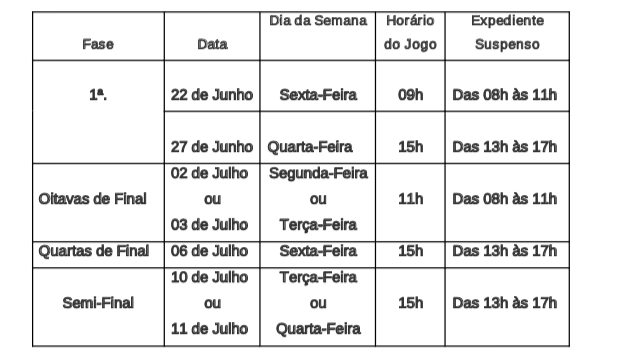
\includegraphics[width=4.56744in,height=2.66667in]{media/image28.png}

Disponível em:
\url{https://www.senges.pr.gov.br/portal/noticias/horario-de-servicos-da-prefeitura-serao-diferenciados-em-dias-de-jogos-do-br/}.
Acesso em: 24 fev. 2023.

Os \textbf{gráficos}, por sua vez, podem ser encontrados em todos os
contextos em que haja necessidade de manipulação de dados, ou seja,
precisem informar dados para transmitir informações ao leitor. Podem ser
veiculados em jornais, revistas, almanaques, artigos científicos, livros
técnicos, \emph{sites} de variedades e diversos outros meios, impressos
ou digitais.

Quem elabora um gráfico, precisa entender muito bem os dados para poder
``traduzi-los'' ao leitor. Um gráfico pode ser feito manualmente, mas
também há ferramentas (programas e aplicativos) em computadores que
facilitam esse trabalho.

Há vários tipos de gráficos. Veja alguns:

Arte: inserir os modelos de gráficos conforme modelos a seguir.
\end{quote}

\begin{longtable}[]{@{}l@{}}
\toprule
\begin{minipage}[t]{0.97\columnwidth}\raggedright\strut
Gráfico de colunas{{[}CHART{]}}

Gráfico de barras

{{[}CHART{]}}

Gráfico de \emph{pizza}

{{[}CHART{]}}\strut
\end{minipage}\tabularnewline
\bottomrule
\end{longtable}

\subsection{Atividades}\label{atividades-8}

\begin{quote}
Explicar aos alunos que este gráfico é conhecido como gráfico de barras.
Caso julgue pertinente, mostre aos alunos como se elabora um gráfico
usando um programa de computador.
\end{quote}

\subsubsection{1. }\label{section-66}

\begin{quote}
Analise o gráfico a seguir, observando sua função e as informações
apresentadas.

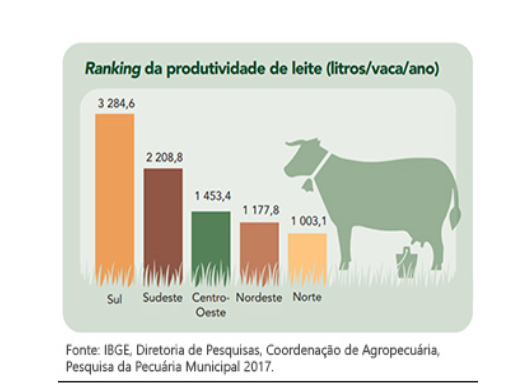
\includegraphics[width=5.68530in,height=4.10069in]{media/image29.png}

IBGE. Tipos de gráficos no ensino. Disponível em:
\textless{}https://educa.ibge.gov.br/professores/educa-recursos/20773-tipos-de-graficos-no-ensino.html\textgreater{}.
Acesso em: 24 fev. 2023.

a) Qual é a finalidade desse gráfico? A finalidade do gráfico é
apresentar ao leitor quanto cada região brasileira produz de leite.

\_\_\_\_\_\_\_\_\_\_\_\_\_\_\_\_\_\_\_\_\_\_\_\_\_\_\_\_\_\_\_\_\_\_\_\_\_\_\_\_\_\_\_\_\_\_\_\_\_\_\_\_\_\_\_\_\_\_\_\_\_\_\_\_

\_\_\_\_\_\_\_\_\_\_\_\_\_\_\_\_\_\_\_\_\_\_\_\_\_\_\_\_\_\_\_\_\_\_\_\_\_\_\_\_\_\_\_\_\_\_\_\_\_\_\_\_\_\_\_\_\_\_\_\_\_\_\_\_

\_\_\_\_\_\_\_\_\_\_\_\_\_\_\_\_\_\_\_\_\_\_\_\_\_\_\_\_\_\_\_\_\_\_\_\_\_\_\_\_\_\_\_\_\_\_\_\_\_\_\_\_\_\_\_\_\_\_\_\_\_\_\_\_

b) Como você chegou a essa conclusão? Espera-se que os alunos que pelo
título do gráfico ``ranking da produtividade de leite'' e pelos nomes
das regiões que estão abaixo das barras: ``Sul, Sudeste, Centro-Oeste,
Nordeste e Norte''.

\_\_\_\_\_\_\_\_\_\_\_\_\_\_\_\_\_\_\_\_\_\_\_\_\_\_\_\_\_\_\_\_\_\_\_\_\_\_\_\_\_\_\_\_\_\_\_\_\_\_\_\_\_\_\_\_\_\_\_\_\_\_\_\_

\_\_\_\_\_\_\_\_\_\_\_\_\_\_\_\_\_\_\_\_\_\_\_\_\_\_\_\_\_\_\_\_\_\_\_\_\_\_\_\_\_\_\_\_\_\_\_\_\_\_\_\_\_\_\_\_\_\_\_\_\_\_\_\_

\_\_\_\_\_\_\_\_\_\_\_\_\_\_\_\_\_\_\_\_\_\_\_\_\_\_\_\_\_\_\_\_\_\_\_\_\_\_\_\_\_\_\_\_\_\_\_\_\_\_\_\_\_\_\_\_\_\_\_\_\_\_\_\_

c) O que as barras presentes no gráfico indicam? As barras indicam que a
diferença entre Nordeste e Norte é menor do que entre Sul e
Centro-Oeste.

Explique aos alunos que um dos recursos gráfico-visuais presente no
gráfico citado são as barras correspondentes a cada região brasileira
que apresentam, em escala, a quantidade de leite produzido em cada uma
delas. Assim, compreende-se, pela altura das barras, que a diferença de
leite produzido entre as regiões Norte e Nordeste é menor do que entre
as regiões Sul e Centro-Oeste, tendo em vista a barra referente à região
Sul é muito maior do que a do Centro-Oeste.

\_\_\_\_\_\_\_\_\_\_\_\_\_\_\_\_\_\_\_\_\_\_\_\_\_\_\_\_\_\_\_\_\_\_\_\_\_\_\_\_\_\_\_\_\_\_\_\_\_\_\_\_\_\_\_\_\_\_\_\_\_\_\_\_

\_\_\_\_\_\_\_\_\_\_\_\_\_\_\_\_\_\_\_\_\_\_\_\_\_\_\_\_\_\_\_\_\_\_\_\_\_\_\_\_\_\_\_\_\_\_\_\_\_\_\_\_\_\_\_\_\_\_\_\_\_\_\_\_

\_\_\_\_\_\_\_\_\_\_\_\_\_\_\_\_\_\_\_\_\_\_\_\_\_\_\_\_\_\_\_\_\_\_\_\_\_\_\_\_\_\_\_\_\_\_\_\_\_\_\_\_\_\_\_\_\_\_\_\_\_\_\_\_

d) Segundo os dados do gráfico, a região Sul está em qual colocação no
\emph{ranking} de maior produtor de leite? Marque a alternativa correta.

( x ) primeiro lugar

( ) segundo lugar

( ) terceiro lugar

( ) quarto lugar

e) A leitura do gráfico é feita da esquerda para a direito. Então, os
resultados são lidos ( x ) do maior produtor de leite (Sul) para o menor
(Norte).

( ) do menor produtor de leite (Norte) para o maior (Sul).

f) Houve regiões com resultados iguais na pesquisa? Justifique sua
resposta. Não. Ao olhar as barras, compreende-se que cada uma tem uma
altura diferente, portanto, os resultados da pesquisa feita pelo gráfico
apontam dados diferentes.

\_\_\_\_\_\_\_\_\_\_\_\_\_\_\_\_\_\_\_\_\_\_\_\_\_\_\_\_\_\_\_\_\_\_\_\_\_\_\_\_\_\_\_\_\_\_\_\_\_\_\_\_\_\_\_\_\_\_\_\_\_\_\_\_

\_\_\_\_\_\_\_\_\_\_\_\_\_\_\_\_\_\_\_\_\_\_\_\_\_\_\_\_\_\_\_\_\_\_\_\_\_\_\_\_\_\_\_\_\_\_\_\_\_\_\_\_\_\_\_\_\_\_\_\_\_\_\_\_

\_\_\_\_\_\_\_\_\_\_\_\_\_\_\_\_\_\_\_\_\_\_\_\_\_\_\_\_\_\_\_\_\_\_\_\_\_\_\_\_\_\_\_\_\_\_\_\_\_\_\_\_\_\_\_\_\_\_\_\_\_\_\_\_

\_\_\_\_\_\_\_\_\_\_\_\_\_\_\_\_\_\_\_\_\_\_\_\_\_\_\_\_\_\_\_\_\_\_\_\_\_\_\_\_\_\_\_\_\_\_\_\_\_\_\_\_\_\_\_\_\_\_\_\_\_\_\_\_
\end{quote}

\subsubsection{2. }\label{section-67}

\begin{quote}
Observe a tabela a seguir das dez empresas mais reclamadas no Procon do
Rio de Janeiro.

Explique aos alunos que o Procon é um órgão que orienta e auxilia os
consumidores na busca pelos seus direitos. Existem Procons espalhados
por todo o território brasileiro.

https://www.minhaoperadora.com.br/2018/07/teles-sao-as-maisreclamadas-no-procon-do-rio-de-janeiro.html

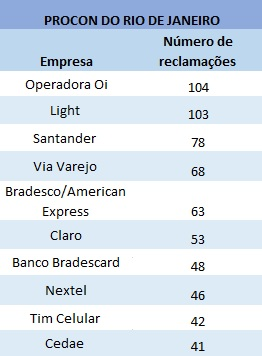
\includegraphics[width=2.72917in,height=3.70833in]{media/image30.jpeg}

Disponível em: \protect\hypertarget{_Hlk128145216}{}{}\textless{}
https://www.minhaoperadora.com.br/2018/07/teles-sao-as-mais-reclamadas-no-procon-do-rio-de-janeiro.html\textgreater{}.
Acesso em: 24 fev. 2023.

a) Qual é o título da tabela? Procon do Rio de Janeiro

\_\_\_\_\_\_\_\_\_\_\_\_\_\_\_\_\_\_\_\_\_\_\_\_\_\_\_\_\_\_\_\_\_\_\_\_\_\_\_\_\_\_\_\_\_\_\_\_\_\_\_\_\_\_\_\_\_\_\_\_\_\_\_\_

\_\_\_\_\_\_\_\_\_\_\_\_\_\_\_\_\_\_\_\_\_\_\_\_\_\_\_\_\_\_\_\_\_\_\_\_\_\_\_\_\_\_\_\_\_\_\_\_\_\_\_\_\_\_\_\_\_\_\_\_\_\_\_\_

b) Segundo dados da tabela, qual foi a empresa mais reclamada pelos
cariocas? A Operadora Oi, com 104 reclamações.

\_\_\_\_\_\_\_\_\_\_\_\_\_\_\_\_\_\_\_\_\_\_\_\_\_\_\_\_\_\_\_\_\_\_\_\_\_\_\_\_\_\_\_\_\_\_\_\_\_\_\_\_\_\_\_\_\_\_\_\_\_\_\_\_

\_\_\_\_\_\_\_\_\_\_\_\_\_\_\_\_\_\_\_\_\_\_\_\_\_\_\_\_\_\_\_\_\_\_\_\_\_\_\_\_\_\_\_\_\_\_\_\_\_\_\_\_\_\_\_\_\_\_\_\_\_\_\_\_

\_\_\_\_\_\_\_\_\_\_\_\_\_\_\_\_\_\_\_\_\_\_\_\_\_\_\_\_\_\_\_\_\_\_\_\_\_\_\_\_\_\_\_\_\_\_\_\_\_\_\_\_\_\_\_\_\_\_\_\_\_\_\_\_

c) E qual foi a empresa com o menor número de reclamações? A Cedae, com
41 reclamações.

\protect\hypertarget{_Hlk128145702}{}{}\_\_\_\_\_\_\_\_\_\_\_\_\_\_\_\_\_\_\_\_\_\_\_\_\_\_\_\_\_\_\_\_\_\_\_\_\_\_\_\_\_\_\_\_\_\_\_\_\_\_\_\_\_\_\_\_\_\_\_\_\_\_\_\_

\_\_\_\_\_\_\_\_\_\_\_\_\_\_\_\_\_\_\_\_\_\_\_\_\_\_\_\_\_\_\_\_\_\_\_\_\_\_\_\_\_\_\_\_\_\_\_\_\_\_\_\_\_\_\_\_\_\_\_\_\_\_\_\_

\_\_\_\_\_\_\_\_\_\_\_\_\_\_\_\_\_\_\_\_\_\_\_\_\_\_\_\_\_\_\_\_\_\_\_\_\_\_\_\_\_\_\_\_\_\_\_\_\_\_\_\_\_\_\_\_\_\_\_\_\_\_\_\_

d) Em sua opinião, essa tabela facilita a organização das informações?
Justifique sua resposta. Espera-se que os alunos respondam que sim, uma
vez que ela organiza e resume os dados.

\_\_\_\_\_\_\_\_\_\_\_\_\_\_\_\_\_\_\_\_\_\_\_\_\_\_\_\_\_\_\_\_\_\_\_\_\_\_\_\_\_\_\_\_\_\_\_\_\_\_\_\_\_\_\_\_\_\_\_\_\_\_\_\_

\_\_\_\_\_\_\_\_\_\_\_\_\_\_\_\_\_\_\_\_\_\_\_\_\_\_\_\_\_\_\_\_\_\_\_\_\_\_\_\_\_\_\_\_\_\_\_\_\_\_\_\_\_\_\_\_\_\_\_\_\_\_\_\_

\_\_\_\_\_\_\_\_\_\_\_\_\_\_\_\_\_\_\_\_\_\_\_\_\_\_\_\_\_\_\_\_\_\_\_\_\_\_\_\_\_\_\_\_\_\_\_\_\_\_\_\_\_\_\_\_\_\_\_\_\_\_\_\_
\end{quote}

\subsection{Treino}\label{treino-8}

\subsubsection{1.}\label{section-68}

(Fácil) Emerson mediu o comprimento dos filhotinhos de sua gatinha,
anotando os dados em uma tabela.

\begin{quote}
Arte: compor tabela conforme modelo
\end{quote}

\begin{longtable}[]{@{}ll@{}}
\toprule
& \textbf{Comprimento em centímetros}\tabularnewline
\midrule
\endhead
Filhote 1 & 10\tabularnewline
Filhote 2 & 11\tabularnewline
Filhote 3 & 12\tabularnewline
Filhote 4 & 9\tabularnewline
Filhote 5 & 10\tabularnewline
\bottomrule
\end{longtable}

Qual foi a medida de comprimento que apareceu mais vezes?

(A) 10 cm.

(B) 12 cm.

(C) 9 cm.

(D) 11 cm.

Saeb D3 - Estabelecer relação entre informações num texto ou entre
diferentes textos.

BNCC: Não há correspondência.

(A) Correta. A medida que mais apareceu foi 10, nos filhotinhos 1 e 5.

(B) Incorreta. A medida 12 cm aparece apenas uma vez.

(C) Incorreta. A medida 9 cm aparece apenas uma vez.

(D) Incorreta. A medida 11 cm aparece apenas uma vez.

\subsubsection{2. }\label{section-69}

(Médio) Fernanda realizou uma pesquisa em sua escola para descobrir quem
joga mais vôlei: meninas ou meninos.

\begin{quote}
Arte: fazer gráfico conforme o modelo. Trocar homens e mulheres por
meninas e meninos. Tirar porcentagem dos números, deixar 53 e 47
\end{quote}

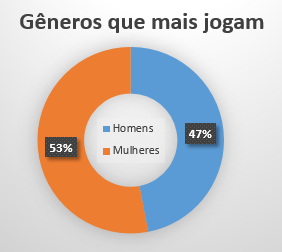
\includegraphics[width=2.60244in,height=2.32558in]{media/image31.png}

Pela pesquisa de Fernanda,

(A) as meninas jogam mais, pois tem 6 a mais que os meninos.

(B) os meninos jogam mais, pois tem 6 a mais que as meninas.

(C) as meninas jogam mais, pois tem 7 a mais que os meninos.

(D) os meninos jogam mais, pois tem 7 a mais que as meninas.

\begin{quote}
Saeb D1 - Localizar informações num texto.

BNCC: Não há correspondência.

(A) Correta. No gráfico, o gênero que mais joga é o das meninas por ser
o maior número. E a diferença entre eles é 6.

(B) Incorreta. O aluno se confundiu ao dizer qual o gênero que mais
joga.

(C) Incorreta. O aluno se confundiu ao dizer a diferença entre os
gêneros.

(D) Incorreta. O aluno se confundiu ao dizer a diferença entre os
gêneros e confundiu a diferença entre eles.
\end{quote}

\subsubsection{3. }\label{section-70}

(Difícil) Em 2015, o IBGE, Instituto Brasileiro de Geografia e
Estatística, fez uma pesquisa em relação à cor, raça e etnia das pessoas
por autodeclaração, ou seja, o próprio entrevistado respondeu a qual
grupo pertence. Observe no gráfico o resultado dessa pesquisa.

\textbf{\textless{}
https://educa.ibge.gov.br/criancas/brasil/nosso-povo/19624-cor-ou-raca.html\textgreater{}.
}

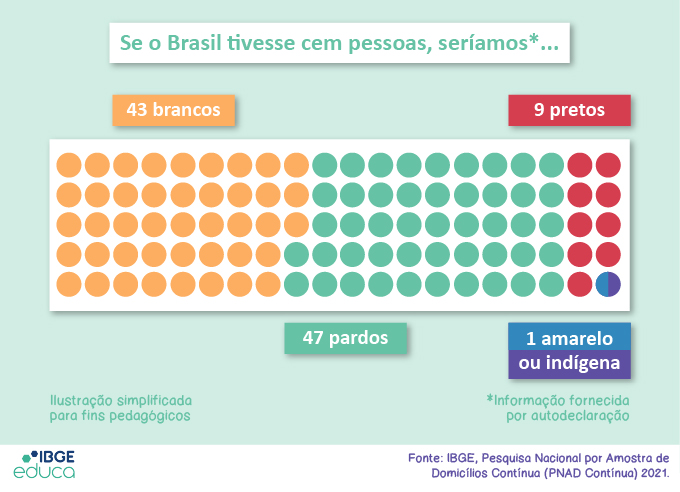
\includegraphics[width=5.51042in,height=3.98702in]{media/image32.jpeg}

\protect\hypertarget{_Hlk40547643}{}{}

Fonte: IBGE. Cor ou raça. Disponível em: \textless{}
https://educa.ibge.gov.br/criancas/brasil/nosso-povo/19624-cor-ou-raca.html\textgreater{}.
Acesso em 24 fev. 2023.

Conforme informações presentes no gráfico, a população do Brasil é
resultado da mistura de diversas raças, e

(A) os de cor parda representam a minoria.

(B) na pesquisa, várias pessoas se autodeclararam amarelas.

(C) metade da população respondeu que é da cor branca.

(D) a cada 100 pessoas entrevistadas, menos de 1 é indígena.

\begin{quote}
Saeb D3 - Estabelecer relação entre informações num texto ou entre
diferentes textos.

BNCC: Não há correspondência.

(A) Incorreta. A cor parda representa 45 pessoas de cada 100
entrevistada.

(B) Incorreta. Menos de 1 por cento se autodeclararam amarelas.

(C) Incorreta. Para ser metade, teriam que ser 50 pessoas e não 45, como
mostra o gráfico.

(D) Correta. Conforme o gráfico, é possível perceber como é a
diversidade populacional brasileira, e por meio da análise dos dados,
afirmar que de cada 100 pessoas entrevistadas menos de 1 é indígena.
\end{quote}

\section{Módulo 10}\label{muxf3dulo-10}

\begin{quote}
Nesta seção, os alunos vão analisar trecho de texto e compreender a
função dos pronomes pessoais; identificar pronomes pessoais no contexto
apresentado; recuperar relações entre partes do texto, identificando
substituições lexicais por pronomes pessoais; identificar em textos a
concordância entre substantivo ou pronome pessoal e verbo (concordância
verbal).
\end{quote}

\subsection{Conteúdo}\label{conteuxfado-9}

\begin{quote}
\url{https://www.istockphoto.com/br/vetor/ilustra\%C3\%A7\%C3\%A3o-conceitual-de-vetor-plano-isom\%C3\%A9trico-3d-do-vocabul\%C3\%A1rio-online-gm1357666281-431507042?utm_source=pixabay\&utm_medium=affiliate\&utm_campaign=SRP_illustration_sponsored\&utm_content=https\%3A\%2F\%2Fpixabay.com\%2Fpt\%2Fillustrations\%2Fsearch\%2Fl\%25C3\%25A9xico\%2F\%3Fmanual_search\%3D1\&utm_term=l\%C3\%A9xico}

\textbf{Pronomes pessoais}

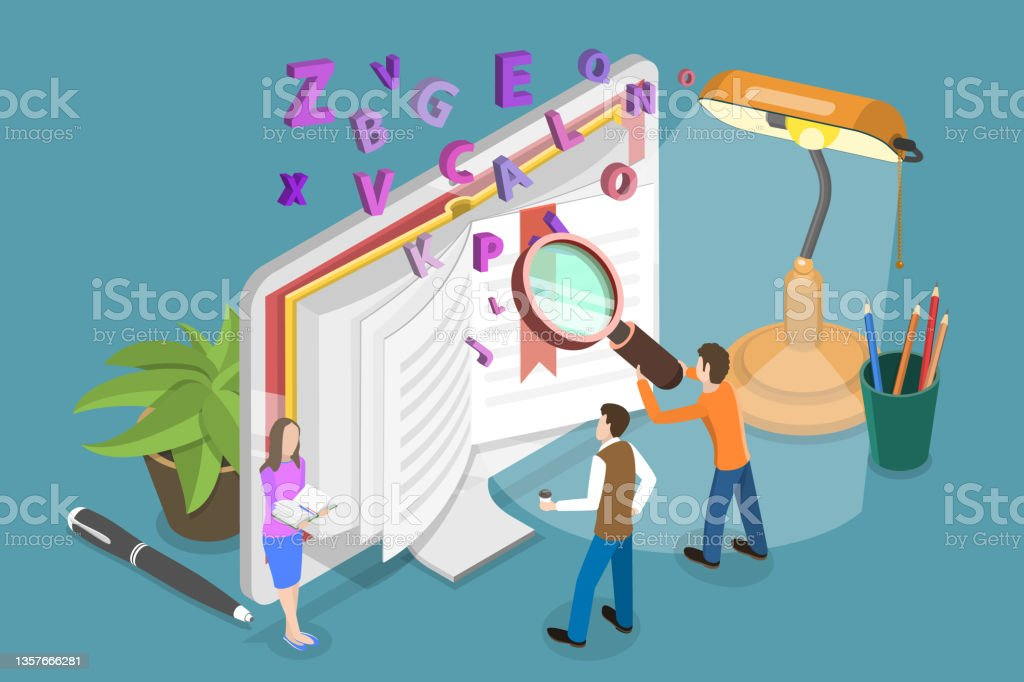
\includegraphics[width=4.81250in,height=3.20531in]{media/image33.jpeg}

Pronome consiste na palavra que substitui ou acompanha um nome, um
substantivo. Pode apresentar variação de gênero e número, de acordo com
o termo ao qual se refere, e desempenhar variadas funções em um texto.

Observe a seguir:
\end{quote}

\begin{longtable}[]{@{}l@{}}
\toprule
\begin{minipage}[t]{0.97\columnwidth}\raggedright\strut
\begin{itemize}
\item
  eu: 1ª pessoa do singular - nós: 1ª pessoa do plural;
\item
  tu: 2ª pessoa do singular - vós: 2ª pessoa do plural;
\item
  ele/ela: 3ª pessoa do singular - eles/elas: 3ª pessoa do plural.
\end{itemize}\strut
\end{minipage}\tabularnewline
\bottomrule
\end{longtable}

\begin{longtable}[]{@{}l@{}}
\toprule
\begin{minipage}[t]{0.97\columnwidth}\raggedright\strut
\begin{quote}
Os pronomes que apontam as pessoas do discurso denominam-se
\textbf{pronomes pessoais}:
\end{quote}

\begin{itemize}
\item
  quem fala -- 1ª pessoa;
\item
  com quem se fala -- 2ª pessoa;
\item
  de quem se fala -- 3ª pessoa.
\end{itemize}\strut
\end{minipage}\tabularnewline
\bottomrule
\end{longtable}

\begin{quote}
A utilização do pronome pessoal permite que o falante indique ao seu
interlocutor aquilo de que se fala (um ser, um objeto, entre outos), que
pode ou não estar presente no momento da interação.

O uso do pronome \textbf{tu} comumente acontece na região Sul do país e
em determinadas localidades das regiões Sudeste, Norte e Nordeste.

Todavia, na oralidade, nem sempre se flexiona o informal verbo na
segunda pessoa. É comum ouvir ``tu comeu'', ``tu sorriu'', que consiste
na variação linguística que ocorre no país.

As palavras utilizadas para nos dirigirmos às pessoas denominam-se
\textbf{pronomes de tratamento}. É o caso de \textbf{você}, uso mais
informal, e de \textbf{senhor} ou \textbf{senhora}, uso mais formal. São
utilizados do mesmo modo que os pronomes pessoais.
\end{quote}

\subsection{Atividades}\label{atividades-9}

\subsubsection{1. }\label{section-71}

\begin{quote}
Leia a narrativa a seguir. Sugere-se propor inicialmente uma leitura
silenciosa. Após a leitura, retomar os aspectos que chamaram a atenção
de cada aluno. Pode-se fazer, em seguida, uma leitura compartilhada,
parágrafo a parágrafo, conversando sobre as palavras desconhecidas e as
impressões relacionadas ao texto.

https://www.istockphoto.com/br/vetor/castelo-com-arquitetura-do-pal\%C3\%A1cio-majestic-e-conto-de-fadas-como-cen\%C3\%A1rio-em-desenho-gm1384445266-443752317?utm\_source=pixabay\&utm\_medium=affiliate\&utm\_campaign=SRP\_illustration\_sponsored\&utm\_content=https\%3A\%2F\%2Fpixabay.com\%2Fpt\%2Fillustrations\%2Fsearch\%2Fprincesa\%2F\%3Fmanual\_search\%3D1\&utm\_term=princesa

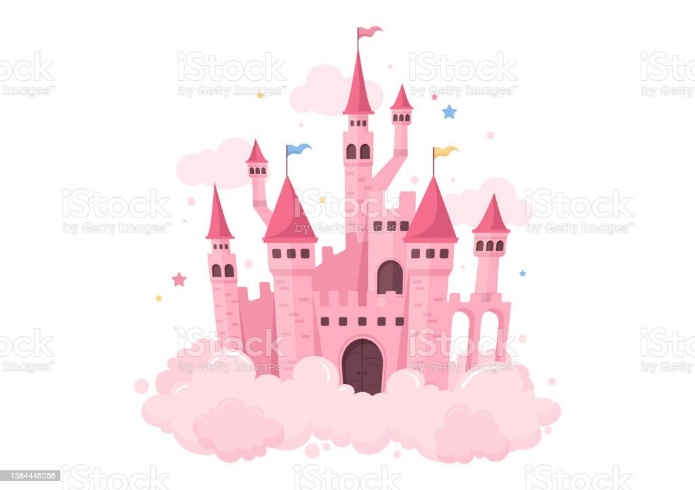
\includegraphics[width=3.15101in,height=2.21875in]{media/image34.jpeg}
\end{quote}

A princesa e a ervilha

~ ~ Era uma vez um príncipe que queria se casar com uma princesa, mas
uma princesa de verdade, de sangue real mesmo. Viajou pelo mundo
inteiro, à procura da princesa dos seus sonhos, mas todas as que ele
encontrava tinha algum defeito. Não é que faltassem princesas, não.
Havia de sobra, mas a dificuldade era saber se realmente eram de sangue
real. E o príncipe retornou ao seu castelo, muito triste e~desiludido,
pois queria muito casar com uma princesa de verdade.

~ ~ Uma noite desabou uma tempestade~medonha. Chovia desabaladamente,
com trovoadas, raios e relâmpagos. Um espetáculo tremendo!

~ ~ De repente bateram à porta do castelo, e o rei em pessoa foi
atender, pois os criados estavam ocupados enxugando as salas cujas
janelas foram abertas pela tempestade.

~ ~ Era uma moça, que dizia ser uma princesa. Mas estava encharcada de
tal maneira, os cabelos escorrendo, as roupas grudadas ao corpo, os
sapatos quase desmanchando\ldots{} que era difícil acreditar que fosse
realmente uma princesa real.

~ ~ A moça tanto afirmou que era uma princesa que a rainha pensou numa
forma de provar se o que ela dizia era verdade.

~ ~ Ordenou que sua criada de confiança empilhasse vinte colchões no
quarto de hóspedes e colocou sob eles uma ervilha. Aquela seria a cama
da ``princesa''.

~ ~ A moça estranhou a altura da cama, mas conseguiu, com a ajuda e uma
escada, se deitar.

~ ~ No dia seguinte, a rainha perguntou como ela havia dormido.

~ ~ -- Oh! Não consegui dormir -- respondeu a moça -- havia algo duro na
minha cama, e me deixou até manchas roxas no corpo!

~ ~ \protect\hypertarget{_Hlk128236047}{}{}O rei, a rainha e o príncipe
se olharam com surpresa. A moça era realmente uma princesa! Só mesmo uma
princesa verdadeira teria pele tão sensível para sentir um grão de
ervilha sob vinte colchões!!!

~ ~ O príncipe casou com a princesa, feliz da vida, e a ervilha foi
enviada para um museu, e ainda deve estar por lá \ldots{}

ANDERSEN, Hans Christian. \textbf{A princesa e a ervilha.} Disponível
em:
\url{https://alfabetizacao.mec.gov.br/images/conta-pra-mim/livros/versao_digital/a_princesa_e_a_ervilha_versao_digital.pdf}.
Acesso em: 25 fev. 2023.

a) Quem são as personagens da história? O príncipe, a princesa, a
rainha, o rei e os empregados.

\_\_\_\_\_\_\_\_\_\_\_\_\_\_\_\_\_\_\_\_\_\_\_\_\_\_\_\_\_\_\_\_\_\_\_\_\_\_\_\_\_\_\_\_\_\_\_\_\_\_\_\_\_\_\_\_\_\_\_\_\_\_\_\_

\_\_\_\_\_\_\_\_\_\_\_\_\_\_\_\_\_\_\_\_\_\_\_\_\_\_\_\_\_\_\_\_\_\_\_\_\_\_\_\_\_\_\_\_\_\_\_\_\_\_\_\_\_\_\_\_\_\_\_\_\_\_\_\_

\_\_\_\_\_\_\_\_\_\_\_\_\_\_\_\_\_\_\_\_\_\_\_\_\_\_\_\_\_\_\_\_\_\_\_\_\_\_\_\_\_\_\_\_\_\_\_\_\_\_\_\_\_\_\_\_\_\_\_\_\_\_\_\_

b) Há quantos parágrafos no texto? 11 parágrafos

\_\_\_\_\_\_\_\_\_\_\_\_\_\_\_\_\_\_\_\_\_\_\_\_\_\_\_\_\_\_\_\_\_\_\_\_\_\_\_\_\_\_\_\_\_\_\_\_\_\_\_\_\_\_\_\_\_\_\_\_\_\_\_\_

c) Qual era o desejo do príncipe? Ele queria se casar com uma princesa
de sangue real.

\_\_\_\_\_\_\_\_\_\_\_\_\_\_\_\_\_\_\_\_\_\_\_\_\_\_\_\_\_\_\_\_\_\_\_\_\_\_\_\_\_\_\_\_\_\_\_\_\_\_\_\_\_\_\_\_\_\_\_\_\_\_\_\_

\_\_\_\_\_\_\_\_\_\_\_\_\_\_\_\_\_\_\_\_\_\_\_\_\_\_\_\_\_\_\_\_\_\_\_\_\_\_\_\_\_\_\_\_\_\_\_\_\_\_\_\_\_\_\_\_\_\_\_\_\_\_\_\_

d) Por que a rainha ordenou que a criada colocasse um grão de ervilha na
cama da princesa? Para se certificar de que a moça era uma princesa de
verdade.

\_\_\_\_\_\_\_\_\_\_\_\_\_\_\_\_\_\_\_\_\_\_\_\_\_\_\_\_\_\_\_\_\_\_\_\_\_\_\_\_\_\_\_\_\_\_\_\_\_\_\_\_\_\_\_\_\_\_\_\_\_\_\_\_

\_\_\_\_\_\_\_\_\_\_\_\_\_\_\_\_\_\_\_\_\_\_\_\_\_\_\_\_\_\_\_\_\_\_\_\_\_\_\_\_\_\_\_\_\_\_\_\_\_\_\_\_\_\_\_\_\_\_\_\_\_\_\_\_

e) Como o rei, a rainha e o príncipe tiveram certeza de que ela era uma
princesa de verdade? Somente uma princesa verdadeira teria pele tão
sensível para sentir um grão de ervilha sob vinte colchões.

\_\_\_\_\_\_\_\_\_\_\_\_\_\_\_\_\_\_\_\_\_\_\_\_\_\_\_\_\_\_\_\_\_\_\_\_\_\_\_\_\_\_\_\_\_\_\_\_\_\_\_\_\_\_\_\_\_\_\_\_\_\_\_\_

\_\_\_\_\_\_\_\_\_\_\_\_\_\_\_\_\_\_\_\_\_\_\_\_\_\_\_\_\_\_\_\_\_\_\_\_\_\_\_\_\_\_\_\_\_\_\_\_\_\_\_\_\_\_\_\_\_\_\_\_\_\_\_\_

\_\_\_\_\_\_\_\_\_\_\_\_\_\_\_\_\_\_\_\_\_\_\_\_\_\_\_\_\_\_\_\_\_\_\_\_\_\_\_\_\_\_\_\_\_\_\_\_\_\_\_\_\_\_\_\_\_\_\_\_\_\_\_\_

\subsubsection{2. }\label{section-72}

Releia o trecho a seguir:

\begin{longtable}[]{@{}l@{}}
\toprule
\begin{minipage}[t]{0.97\columnwidth}\raggedright\strut
~ ~

A moça tanto afirmou que era uma princesa que a rainha pensou numa forma
de provar se o que ela dizia era verdade.\strut
\end{minipage}\tabularnewline
\bottomrule
\end{longtable}

\begin{itemize}
\item
  A palavra ela no trecho se refere
\end{itemize}

( x ) à moça ( ) à rainha

\subsubsection{3. }\label{section-73}

Siga o exemplo e escreva a forma verbal que corresponde à pessoa
destacada e complete as frases.

\begin{longtable}[]{@{}l@{}}
\toprule
\textbf{Eu dormi} sob a ervilha.\tabularnewline
\bottomrule
\end{longtable}

a) Nós \_\_dormimos\_\_\_\_\_\_\_\_\_\_\_\_\_\_ sob a ervilha.

b) Vocês \_\_\_\_dormiram\_\_\_\_\_\_\_\_\_\_ sob a ervilha.

c) Eles \_\_\_\_\_dormiram\_\_\_\_\_\_\_\_\_\_\_\_ sob a ervilha.

d) Você \_\_\_\_\_dormiu\_\_\_\_\_\_\_\_\_\_\_\_ sob a ervilha.

e) Ele \_\_\_\_\_\_\_dormiu\_\_\_\_\_\_\_ sob a ervilha

\subsubsection{4. }\label{section-74}

Substitua os termos destacados pelos pronomes pessoais adequados.

a) \textbf{O príncipe} casou com a princesa. Ele

\_\_\_\_\_\_\_\_\_\_\_\_\_\_\_\_\_\_\_\_\_\_\_\_\_\_\_\_\_\_\_\_\_\_\_\_\_\_\_\_\_\_\_\_\_\_\_\_\_\_\_\_\_\_\_\_\_\_\_\_\_\_\_\_

b) \textbf{O rei e a rainha} gostaram da princesa\textbf{.} Eles

\_\_\_\_\_\_\_\_\_\_\_\_\_\_\_\_\_\_\_\_\_\_\_\_\_\_\_\_\_\_\_\_\_\_\_\_\_\_\_\_\_\_\_\_\_\_\_\_\_\_\_\_\_\_\_\_\_\_\_\_\_\_\_\_

c) \textbf{O rei, a rainha e o príncipe} se olharam com surpresa. Eles

\_\_\_\_\_\_\_\_\_\_\_\_\_\_\_\_\_\_\_\_\_\_\_\_\_\_\_\_\_\_\_\_\_\_\_\_\_\_\_\_\_\_\_\_\_\_\_\_\_\_\_\_\_\_\_\_\_\_\_\_\_\_\_\_

d) \textbf{Eu e a princesa} casamos. Nós

\_\_\_\_\_\_\_\_\_\_\_\_\_\_\_\_\_\_\_\_\_\_\_\_\_\_\_\_\_\_\_\_\_\_\_\_\_\_\_\_\_\_\_\_\_\_\_\_\_\_\_\_\_\_\_\_\_\_\_\_\_\_\_\_

\subsubsection{5. }\label{section-75}

Releia as frases da atividade anterior, substituindo os termos
destacados pelos pronomes. A substituição dos pronomes altera os verbos?
Espera-se que os alunos percebam que não, os verbos permanecem, tendo em
vista que os pronomes substituem os termos destacados sem alterar as
pessoas do discurso.

\subsubsection{6. }\label{section-76}

Qual é a função dos termos que você usou na atividade 4?

\begin{quote}
( ) Indicar uma ação.

( x ) Substituir os nomes.
\end{quote}

\subsection{Treino}\label{treino-9}

\subsubsection{1.}\label{section-77}

\begin{quote}
(Fácil) Leia a charadinha a seguir.
\end{quote}

\begin{longtable}[]{@{}l@{}}
\toprule
\begin{minipage}[t]{0.97\columnwidth}\raggedright\strut
\begin{quote}
Por que a mula não usa chapéu? Porque ela não tem cabeça.
\end{quote}\strut
\end{minipage}\tabularnewline
\bottomrule
\end{longtable}

\begin{quote}
A palavra ``ela'' se refere a

(A) ``chapéu''.

(B) ``cabeça''.

(C) ``mula''.

(D) ``tem''.

Saeb D2 - Inferir uma afirmação implícita num texto.

BNCC Não há correspondência.

(A) Incorreta. A palavra ``ela'' não pode retomar ``chapéu''.

(B) Correta. A palavra ``ela'' não pode retomar ``cabeça''.

(C) Correta. O pronome ``ela'' está substituindo a palavra ``mula'',

(D) Incorreta. Pronomes retomam substantivos, e não verbos.
\end{quote}

\subsubsection{2. }\label{section-78}

\begin{quote}
(Médio) Leia a campanha publicitária a seguir.

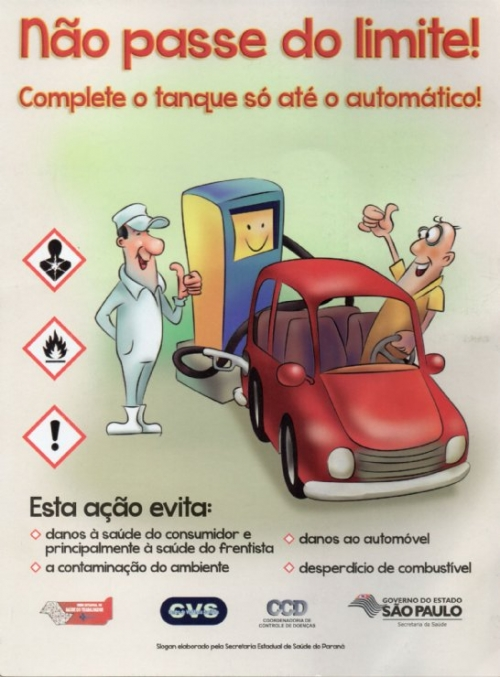
\includegraphics[width=5.20833in,height=7.05556in]{media/image35.jpeg}

GOVERNO DE OURINHOS. Vigilância sanitária alerta frentistas sobre a
campanha educativa ``Não passe do limite! Complete o tanque só até o
automático''. Disponível em:
\textless{}www.ourinhos.sp.gov.br/noticia/1910/vigilancia-sanitaria-alerta-frentistas-sobre-a-campanha-educativa-nao-passe-do-limite-complete-o-tanque-so-ate-o-automatico/\textgreater{}.
Acesso em: 25 fev. 2023.

Na frase ``Esta ação evita'', a palavra ``esta'' está se referindo

(A) ao ``desperdício de combustível''.

(B) a ``não passe do limite''.

(C) a ``complete o tanque até o automático''.

(D) a ``danos à saúde do consumidor''.

Saeb D2 - Inferir uma afirmação implícita num texto.

BNCC Não há correspondência.

(A) Incorreta. O ``desperdício de combustível'' é uma das consequências
a serem evitadas com essa ação.

(B) Incorreta. O pronome não tem relação com essa frase.

(C) Correta. O pronome demonstrativo ``esta'', refere-se a ``completar o
tanque só até o automático''.

(D) Incorreta. O pronome não se refere a ``danos à saúde''.
\end{quote}

\subsubsection{3. }\label{section-79}

(Difícil) Leia o trecho da reportagem sobre pais e filhos.

\begin{quote}
\textbf{Assando pães e pizzas, pais e filhos descobrem prazer de
cozinhar juntos}

A vida de Sofia Santos Vasconcelos, 10, era diferente e quase sem graça,
como ela diz. Entre receitas e pratos, podia, no máximo, ajudar com
colheradas de açúcar e farinha. Com a quarentena e mais tempo ao lado da
mãe, tudo mudou da água para o vinho.

{[}...{]}

Tudo começou comigo e meu marido pensando em como ocupar o tempo dela.
Um dia vi uma receita muito legal de pizza com farinha de amêndoas.
Resolvemos fazer'', lembra a mãe. ``Ficou maravilhosa, e passei a
incentivá-la a buscar mais''.

FRANCO, Marcella. Assando pães e pizzas, pais e filhos descobrem prazer
de cozinhar juntos.

Disponível em:
https://www1.folha.uol.com.br/folhinha/2020/05/assando-paes-e-pizzas-pais-e-filhos-descobrem-prazer-de-cozinhar-juntos.shtml.
Acesso em: 25 fev. 2023.

No trecho ``passei a incentivá-la a buscar mais'', ``la'' está sendo
usado no lugar

da palavra

(A) ``receita''.

(B) ``mãe''.

(C) ``Sofia''.

(D) ``maravilhosa''.

Saeb D2 - Inferir uma afirmação implícita num texto.

BNCC Não há correspondência.

(A) Incorreta. O pronome não está retomando ``receita''.

(B) Incorreta. O pronome não está retomando ``mãe''.

(C) Correta. ``la'' está substituindo ``Sofia''.

(D) Incorreta. O pronome não pode retomar um substantivo.
\end{quote}

\section{Simulado 1}\label{simulado-1}

\subsubsection{1. }\label{section-80}

\begin{quote}
Leia o trecho da notícia.

\textbf{Peça primorosa da Cia. Delas, ``Maria e os Insetos''; retrata
cientista como heroína}

Depois de ``Mary e os Monstros Marinhos'', a Cia. Delas volta com o tema
da invisibilidade das mulheres na ciência em ``Maria e os Insetos''.
Dirigida por uma das integrantes do grupo, Thaís Medeiros, a peça marca
a maturidade da companhia de mulheres, que estreou em 2001 trazendo o
universo de Clarice Lispector para crianças.

Com gestos coreografados que bem desenham mundos interiores​, as atrizes
Fernanda Castello Branco, Julia Ianina e Paula Weinfeld se revezam de
modo dinâmico no papel da protagonista, Maria Sibylla Merian,
ilustradora científica nascida na Alemanha, em 1647 --- uma mulher que
foi tão pioneira quanto esquecida em tudo o que fez.

ROMEU, Gabriela. Peça primorosa da Cia. Delas, ``Maria e os Insetos.
Disponível em:
https://guia.folha.uol.com.br/crianca/2020/02/peca-primorosa-da-cia-delas-maria-e-os-insetos-retrata-cientista-como-heroina.shtml.
Acesso em: 26 fev. 2023.

\textbf{primorosa}: encantadora.

O tema do texto é

(A) a Cia. Delas.

(B) a peça ``Maria e os Insetos''.

(C) o tema ``Mary e os monstros marinhos''.

(D) o grupo de Thaís Medeiros.

Saeb D1 - Localizar informações num texto.

BNCC EF35LP03: Identificar a ideia central do texto, demonstrando
compreensão global.

(A) Incorreta. Cia. Delas são os criadores da peça.

(B) Correta. A notícia trata em relação à peça ``Maria e os Insetos'',
criada pela Cia. Delas.

(C) Incorreta. ``Mary e os monstros marinhos'' é uma das peças criada
pela mesma companhia.

(D) Incorreta. Thaís Medeiros faz parte da Cia. Delas, grupo que criou a
peça ``Maria e os insetos'', tema da notícia.
\end{quote}

\subsubsection{2. }\label{section-81}

O texto a seguir conta a história de um acordo feito entre quatro
animais. Leia-o.

\textbf{O leão, a vaca, a cabra e a ovelha}

Um leão, uma vaca, uma cabra e uma ovelha combinaram de caçar juntos e
repartir o que conseguissem. {[}\ldots{}{]} logo, repartiram a carne em
quatro partes. o leão se apossou da primeira parte, dizendo:

--- esta é minha, como combinamos.

O LEÃO, a vaca, a cabra e a ovelha. Disponível em:
\textless{}www.dominiopublico.gov.br/download/texto/me000589.pdf\textgreater{}.
Acesso em: 27 fev. 2023.

Com quem ficou a primeira parte carne? Marque a alternativa correta.

\begin{quote}
(A) Com a ovelha.

(B) Com a cabra.

(C) Com a vaca.

(D) Com o leão.

Saeb D2 - Inferir uma afirmação implícita num texto.

BNCC EF15LP03: Localizar informações explícitas em textos.

(A) Incorreta. A ovelha não ficou com a minha primeira parte, foi o
leão.

(B) Incorreta. A cabra não ficou com a primeira parte da carne.

(C) Incorreta. A vaca não ficou com a primeira parte da carne.

(D) Correta. O texto deixa explícito que o animal que ficou com a
primeira parte da carne foi o leão, como visto em: ``o leão se apossou
da primeira parte''.
\end{quote}

\subsubsection{3. }\label{section-82}

\begin{quote}
Viagens de Gulliver é um livro em que se relata as viagens da personagem
principal, Gulliver. Leia um trecho.

\textbf{Viagens de Gulliver}

{[}\ldots{}{]} Desconheço qual tivesse sido a sorte dos meus
companheiros de lancha, nem dos que se salvaram do escolho,
{[}\ldots{}{]} mas desconfio que pereceram todos; quanto a mim nadei ao
acaso e fui levado para a terra pelo vento e pela maré. De vez em quando
estendia as pernas para ver se encontrava o fundo; por fim, estando
quase exausto, tomei pé. Por então, o temporal amainara {[}\ldots{}{]}
caminhei perto de meia légua pelo mar, antes que pusesse pé em terra
firme.

SWIFT, Jonathan. Viagens de Gulliver. Disponível em:

www.dominiopublico.gov.br/download/texto/ph000001.pdf. Acesso em: 27
fev. 2023.

\textbf{escolho}: rocha

\textbf{pereceram}: morreram

\textbf{amainara}: acalmara

Com base na leitura do trecho, a lancha

(A) colidiu com uma rocha e afundou.

(B) levou a personagem à praia.

(C) tinha só um tripulante.

(D) navegava em um dia de tempo bom.

Saeb D2 - Inferir uma afirmação implícita num texto.

BNCC EF35LP04: Inferir informações implícitas nos textos lidos.

(A) Correta. A lancha que levava a tripulação colidiu com uma rocha, e
afundou, o que pode ser inferido pela leitura de ``mas desconfio que
pereceram todos; quanto a mim nadei ao acaso e fui levado para a terra
pelo vento e pela maré''.

(B) Incorreta. A personagem chegou a nado até o local, visto que a
lancha afundou.

(C) Incorreta. Não tinha somente um tripulante na lancha.

(D) Incorreta. A lancha navegada em um dia de chuva.
\end{quote}

\subsubsection{4. }\label{section-83}

\begin{quote}
O conto ``Os sete corvos'' narra a história de um casal que teve os sete
filhos transformados em corvos. Leia o início do conto.

\textbf{Os sete corvos}

Era uma vez um homem que tinha sete filhos, todos meninos, e vivia
suspirando por uma menina. Afinal, um dia, a mulher anunciou-lhe que
estava mais uma vez esperando criança.

No tempo certo, quando ela deu à luz, veio uma menina. Foi imensa a
alegria deles. Mas, ao mesmo tempo, ficaram muito preocupados, pois a
recém-nascida era pequena e fraquinha, e precisava ser batizada com
urgência.

Então, o pai mandou um dos filhos ir bem depressa até a fonte e trazer
água para o batismo. O menino foi correndo e, atrás dele, seus seis
irmãos. Chegando lá, cada um queria encher o cântaro primeiro; na
disputa, o cântaro caiu na água e desapareceu.

{[}\ldots{}{]}

IRMÃOS GRIMM. \textbf{Os sete corvos}. Disponível em:

www.dominiopublico.gov.br/download/texto/me001614.pdf. Acesso em: 26
fev. 2023.

\textbf{cântaro}: jarra para guardar água.

A expressão ``estava mais uma vez esperando criança'' significa que

(A) os filhos não tinham voltado.

(B) o pai e a mãe esperavam mais um menino.

(C) a mulher estava grávida.

(D) a mulher não sabia onde era a fonte.

Saeb D5 - Inferir o sentido de uma palavra ou expressão a partir do
contexto imediato.

BNCC EF35LP05 - Inferir o sentido de palavras ou expressões
desconhecidas em textos, com base no contexto da frase ou do texto.

(A) Incorreta. Essa informação não se refere à expressão destacada.

(B) Incorreta. No texto, verifica-se que os pais estavam, dessa vez,
esperando uma menina.

(C) Correta. Infere-se que, ao estar ``esperando criança'', a mãe estava
grávida novamente.

(D) Incorreta. Essa informação não se refere à expressão destacada.
\end{quote}

\section{Simulado 2}\label{simulado-2}

\subsubsection{1. }\label{section-84}

\begin{quote}
Leia os dois textos a seguir, que apresentam trechos finais de duas
narrativas.

\textbf{I}

Chapeuzinho vermelho

{[}\ldots{}{]} --- Vovó, como são grandes os seus dentes!

--- É para te comer!

E assim dizendo, o malvado lobo se atirou sobre Chapeuzinho Vermelho e a
comeu.

PERRAULT, Charles. Chapeuzinho vermelho. Disponível em:

\href{http://www.dominiopublico.gov.br/download/texto/me000589.pdf}{www.dominiopublico.gov.br/download/texto/me000589.pdf}.
Acesso em: 27 fev. 2023.

\textbf{II}

\textbf{Chapeuzinho vermelho}

{[}\ldots{}{]} --- Oh, vovozinha, que boca enorme você tem!

--- É para engolir você melhor!!!

Assim dizendo, o lobo mau deu um pulo e, num movimento só, comeu a pobre
Chapeuzinho Vermelho. {[}\ldots{}{]}

Algumas horas mais tarde, um caçador passou em frente à casa da vovó,
ouviu o barulho e pensou: ``Olha só como a velhinha ronca! Estará
passando mal!? Vou dar uma espiada.''

Abriu a porta, chegou perto da cama e\ldots{} quem ele viu?

O lobo, que dormia como uma pedra, com uma enorme barriga parecendo um
grande balão!

O caçador ficou bem satisfeito. Há muito tempo estava procurando esse
lobo, que já matara

muitas ovelhas e cordeirinhos.

--- Afinal você está aqui, velho malandro! Sua carreira terminou. Já vai
ver! {[}\ldots{}{]}

IRMÃOS GRIMM. Chapeuzinho vermelho. Disponível em:

www.dominiopublico.gov.br/download/texto/me000589.pdf. Acesso em: 27
fev. 2023.

Os dois textos estabelecem uma relação entre si, sendo que o texto II
apresenta características do gênero textual

(A) reconto, porque traz novas informações à primeira versão.

(B) anedota, porque tem o objetivo de provocar o riso do leitor.

(C) poema visual, porque a história é narrada por meio de imagens.

(D) fábula, porque apenas as personagens animais falam.

Saeb D3 - Estabelecer relação entre informações num texto ou entre
diferentes textos.

BNCC EF35LP29: Identificar, em narrativas, cenário, personagem central,
conflito gerador, resolução e o ponto de vista com base no qual
histórias são narradas, diferenciando narrativas em primeira e terceira
pessoas.

(A) Correta. A versão de ``Chapeuzinho vermelho'' dos Irmãos Grimm
mostra um novo final para a narrativa tradicional, na qual a história
termina quando o Lobo Mau come a Chapeuzinho vermelho, caracterizando um
reconto.

(B) Incorreta. O texto II não apresenta uma construção de humor.

(C) Incorreta. Não há características de poema visual.

(D) Incorreta. O texto apresenta personagens humanos que falam, como a
Chapeuzinho Vermelho e o caçador.
\end{quote}

\subsubsection{2. }\label{section-85}

\begin{quote}
Leia o trecho que traz um diálogo entre os personagens Lola, o Gerente e
Gouveia, da peça teatral de Artur Azevedo, A capital federal.

\textbf{A capital federal}

{[}\ldots{}{]}

--- Cena VI ---

{[}\ldots{}{]}

Lola (Entrando.) --- Então? Estou esperando há uma hora!...

{[}\ldots{}{]}

Lola --- {[}\ldots{}{]} O que eu quero é falar ao Gouveia!

O Gerente --- Já o mandei chamar. (Vendo o Gouveia que desce a escada.)
E ele aí vem descendo a escada. {[}\ldots{}{]} (Sai.)

Gouveia (Que tem descido.) --- {[}\ldots{}{]} Não te disse que não me
procurasses aqui? Este hotel...

AZEVEDO, Artur. A capital federal. Disponível em:

www.dominiopublico.gov.br/download/texto/bn000020.pdf. Acesso em: 27
fev. 2023.

Peças teatrais devem ser encenadas por atores em teatros. Elas são
parecidas com

(A) entrevista.

(B) reportagem.

(C) roteiro de cinema.

(D) jornal de rádio.

Saeb D3 - Estabelecer relação entre informações num texto ou entre
diferentes textos.

BNCC EF35LP29: Identificar, em narrativas, cenário, personagem central,
conflito gerador, resolução e o ponto de vista com base no qual
histórias são narradas, diferenciando narrativas em primeira e terceira
pessoas.

(A) Incorreta. Entrevistas são gêneros informativos que podem ser
veiculados por variados meios de comunicação e têm entrevistador e
entrevistado.

(B) Incorreta. Reportagens são textos informativos veiculados por vários
meios de comunicação, os quais têm informações reais e atuais.

(C) Correta. Roteiros de cinema, como as peças teatrais, são escritos
para serem encenados por atores em filmes.

(D) Incorreta. Jornal radiofônico é aquele que transmite as notícias da
atualidade por meio de uma rádio.
\end{quote}

\subsubsection{3. }\label{section-86}

\begin{quote}
Leia o trecho a seguir que mostra uma entrevista com um químico que
trabalha no Centro de Tecnologia de Chocolate da Nestlé, na Inglaterra.

\textbf{Doutor chocolate}

\textbf{CHC:\emph{~Para muitos, o senhor tem o melhor emprego do mundo.
O senhor come chocolate todos os dias?}}\\
Josélio Vieira:~Além de ser o melhor emprego do mundo, trabalhar com
chocolate é fascinante do ponto de vista científico. As tecnologias
estão cada vez mais sofisticadas! Não digo que como chocolates todos os
dias, mas muitas das reuniões envolvem degustar várias amostras.
{[}...{]}

\emph{\textbf{Como é seu dia a dia?}}\\
Sou responsável pela busca de novas tecnologias e por fornecer
direcionamento e conselhos técnicos a projetos de desenvolvimento de
produtos. Meu dia a dia é repleto de reuniões com técnicos internos e
externos. {[}...{]}

Doutor chocolate. \textbf{CHC}. Disponível em:
\url{https://chc.org.br/doutor-chocolate/}. Acesso em: 27 fev. 2023.

Na entrevista, os trechos em negrito são as

(A) perguntas do entrevistador.

(B) respostas do entrevistado.

(C) informações sobre o chocolate.

(D) falas dos personagens.

Saeb D4 - Identificar o tema central do texto.

BNCC EF35LP16: Identificar e reproduzir, em notícias, manchetes, lides e
corpo de notícias simples para público infantil e cartas de reclamação
(revista infantil), digitais ou impressos, a formatação e diagramação
específica de cada um desses gêneros, inclusive em suas versões orais.

.

(A) Correta. Em entrevistas, as perguntas feitas pelo entrevistador
normalmente são apresentadas em negrito para que possam ser
diferenciadas das respostas do entrevistado.

(B) Incorreta. As respostas do entrevistado normalmente são apresentadas
da forma normal, sem estar em negrito.

(C) Incorreta. Os trechos em negrito não mostram esse assunto.

(D) Incorreta. Essa é uma característica de um texto narrativo e não de
um texto informativo como a entrevista.
\end{quote}

\subsubsection{4. }\label{section-87}

\begin{quote}
Observe como fazer uma peteca de palha de banana no texto a seguir.

\textbf{Descubra como fazer uma peteca usando palha de banana}

Não é só de palha de milho que vivem as petecas pelo Brasil. Em Abadia
(Minas Gerais), as meninas usam a casca da bananeira para
confeccioná-las.

Siga os passos {[}\ldots{}{]}:

1. Pegue um pouco de cascas da bananeira.

2. Dobre uma parte da casca até que fique com um volume pequeno.

3. Corte um outro pedaço da casca e embrulhe numa trouxinha o volume da
casca que está

dobrado.

4. Amarre com fios da própria casca ou barbante para amarrar a ponta da
peteca.

5. Depois de amarrada, coloque penas {[}\ldots{}{]} na ponta.

E pronto.

MEIRELLES, Renata. Descubra como fazer uma peteca usando palha de
banana. EBC. Disponível

em:
www.ebc.com.br/infantil/2016/11/descubra-como-fazer-uma-peteca-usando-palha-de-banana.

Acesso em: 27 fev. 2023 (Adaptado).

confeccioná-las: fabricar, produzir, fazer.

Qual é a finalidade do texto?

(A) Explicar que as petecas foram inventadas em Abadia, Minas Gerais.

(B) Instruir como se faz uma peteca com a casca da bananeira.

(C) Mostrar como se faz uma peteca de palha de milho.

(D) Explicar a origem das petecas de palha de milho.

Saeb D7 - Relacionar, na compreensão do texto, informações textuais com
conhecimentos de senso comum.

BNCC EF03LP11: Ler e compreender, com autonomia, textos injuntivos
instrucionais (receitas, instruções de montagem etc.), com a estrutura
própria desses textos (verbos imperativos, indicação de passos a ser
seguidos) e mesclando palavras, imagens e recursos gráfico- visuais,
considerando a situação comunicativa e o tema/assunto do texto.

(A) Incorreta. A finalidade do texto, além de ensinar a se fazer petecas
de palha de bananeira, é mostrar que a origem delas é de Abadia, Minas
Gerais, e não explicar a invenção do brinquedo.

(B) Correta. Pela leitura do trecho, pode-se compreender que a
finalidade do texto é instruir o leitor a montar uma peteca a partir da
casca de bananeira, o que pode ser observado pelo uso das instruções
passo a passo.

(C) Incorreta. O texto mostra como se faz uma peteca com a palha de
bananeira, e não de palha de milho.

(D) Incorreta. O texto apresenta a origem e o modo de se confeccionar
uma peteca de palha de banana, em oposição à peteca de palha de milho.
\end{quote}

\section{Simulado 3}\label{simulado-3}

\subsubsection{1. }\label{section-88}

\begin{quote}
Leia o texto a seguir.

\textbf{O assustador livro vermelho}

No final de 2014, foi publicado um dos livros mais aterrorizantes que
nós já lemos: o livro vermelho. Não é uma história de terror comum, com
monstros ou facas, e sim a lista dos animais brasileiros ameaçados de
extinção. Pesquisadores estudaram 12.256 animais de todos os tipos e
viram que quase uma espécie em cada dez está ameaçada. {[}...{]}

No Brasil, a instituição responsável por realizar esta pesquisa é~o
Instituto Chico Mendes de Conservação da Biodiversidade~(ICMBio). Um
trabalho \textbf{ingrato}, não acha? Mas muito importante. Afinal,
conhecendo exatamente as ameaças à nossa fauna, podemos pensar em
soluções para preservá-la.

O assustador livro vermelho. CHC. Disponível em:
\url{https://chc.org.br/o-assustador-livro-vermelho/}. Acesso em: 28
fev. 2023.

A palavra em destaque é formada pela junção de duas partes. A mesma
formação de palavras ocorre na palavra

(A) triste.

(B) felizes.

(C) informal.

(D) inveja.

Saeb D5 - Inferir o sentido de uma palavra ou expressão a partir do
contexto imediato.

BNCC EF03LP10 - Reconhecer prefixos e sufixos produtivos na formação de
palavras derivadas de substantivos, de adjetivos e de verbos,
utilizando-os para compreender palavras e para formar novas palavras.

(A) Incorreta. A palavra ``triste'' não é formada pela junção de duas
partes como acontece em ``ingrato''.

(B) Incorreta. A palavra ``felizes'' não é formada pela junção de duas
partes, como acontece em ``ingrato''.

(C) Correta. A palavra destacada é feita pela junção do prefixo ``in''
mais a palavra ``grato''. Assim, o mesmo ocorre em ``informal'' em que
se tem a junção de ``in'' com a palavra ``formal'', dando a ela um novo
sentido.

(D) Incorreta. A palavra ``inveja'' não é formada pela junção de duas
partes, como acontece na palavra ``ingrato''. O aluno que marca essa
alternativa reparou apenas no começo de ambas as palavras, que
apresentam ``in'', sem compreender que na palavra ``inveja'' não há a
junção de ``in'' mais ``veja''.
\end{quote}

\subsubsection{2. }\label{section-89}

\begin{quote}
O trecho a seguir é o início do conto \textbf{Ali Babá e os quarenta
ladrões}, leia para compreender como o personagem convivia com todos.

\textbf{Ali Babá e os quarenta ladrões}

Numa distante cidade do Oriente, vivia um homem bom e justo, chamado Ali
Babá.

Ali Babá era muito pobre. Morava numa tenda, entre um vasto deserto e um
grande oásis. Para sustentar a mulher, Samira, e os quatro filhos, Ali
Babá oferecia seus serviços às caravanas de mercadores que passavam por
ali. Estava sempre pronto para cuidar dos camelos, lavá-los, escová-los
e dar-lhes água e alimento.

Os ricos comerciantes já conheciam Ali Babá e gostavam muito de seu
serviço. Ele sempre cobrava o preço justo pelo trabalho, porém, muitas
vezes, os mercadores davam-lhe mais, pois sabiam que ele vivia em
dificuldades.

{[}\ldots{}{]}

ALI BABÁ e os quarenta ladrões. Disponível em:
www.dominiopublico.gov.br/download/texto/me001614.pdf. Acesso em: 28
fev. 2023.

\textbf{oásis}: pequena região fértil no deserto, com presença de água.

\textbf{caravanas}: grupos de mercadores viajantes.

Considerando-se o trecho, Ali Babá

\protect\hypertarget{_Hlk128465624}{}{}(A) trabalhava para os
comerciantes ricos.

(B) cuidava dos camelos de Samira e seus quatro filhos.

(C) cobrava um preço mais alto dos mercadores.

(D) entregava água e alimento para os mercadores venderem.

Saeb D2 - Inferir uma afirmação implícita num texto.

BNCC EF35LP04 - Inferir informações implícitas nos textos lidos.

(A) Correta. Ali Babá trabalhava para comerciantes ricos, informação
implícita no trecho ``Os ricos comerciantes já conheciam Ali Babá e
gostavam muito de seu serviço''.

(B) Incorreta. Os camelos eram dos ricos comerciantes.

(C) Incorreta. Os mercadores davam dinheiro a mais para Ali Babá por
terem simpatia com ele.

(D) Incorreta. A água e o alimento eram para os camelos dos viajantes.
\end{quote}

\subsubsection{3. }\label{section-90}

\begin{quote}
Leia o trecho que conta a história de um reino e seus moradores.

\textbf{No reino das letras felizes}

Num lugar muito distante, existia um reino silencioso, habitado apenas
por letras. Elas eram muito desunidas: vivia cada uma para si, e nunca
se reuniam para formar uma palavra sequer.

HECK, Lenira Almeida. No reino das letras felizes. Disponível em:

www.dominiopublico.gov.br/download/texto/eu00005a.pdf. Acesso em: 28
fev. 2023.

No reino silencioso moravam

(A) letras felizes.

(B) letras desunidas.

(C) animais silenciosos.

(D) palavras formadas.

Saeb D1 - Localizar informações num texto.

BNCC EF15LP03 - Localizar informações explícitas em textos.

(A) Incorreta. O reino era das letras felizes.

(B) Correta. Os habitantes do ``reino silencioso'' eram letras
desunidas.

(C) Incorreta. Não há animais mencionados.

(D) Incorreta. As palavras não moravam nesse reino.

\textbf{4.}

O conto ``O avô e o netinho'', de Figueiredo Pimentel, conta a história
de tio Benedito.

\textbf{O avô e o netinho}

{[}...{]}

Bastante velho já, fatigado por uma longa existência de trabalhos e
canseiras, exausto de forças e doente de velhice -- porque a velhice é,
também, uma doença -- estava tio Benedito, o bom e estimado velhote tio
Benedito: oitenta anos pesavam-lhe às costas, como um grande fardo que
ele a custo carregasse.

Na sua mocidade, e mesmo durante parte da velhice, ninguém trabalhara
mais que ele, honesto sempre, mourejando, dia e noite, para sustento de
sua família.

Não podendo fazer serviço algum, alquebrado pela idade, veio morar em
casa de Augusto, seu filho mais moço, já com um filhinho de três para
quatro anos, o pequenino e interessante Luís, vivo e esperto como
poucos.

PIMENTEL, Figueiredo. O avô e o netinho. Disponível em:

www.dominiopublico.gov.br/download/texto/bn000137.pdf. Acesso em: 28
fev. 2023.

fatigado: cansado

mourejando: trabalhando muito

alquebrado: abatido; cansado

A ideia central do trecho apresentado é

(A) mostrar a família do tio Benedito.

(B) mostrar o que é a velhice.

(C) explicar o título do conto.

(D) apresentar o tio Benedito.

Saeb D4 - Identificar o tema central do texto.

BNCC EF35LP03 - Identificar a ideia central do texto, demonstrando
compreensão global.

(A) Incorreta. Só se mencionou a família para mostrar com quem ele vai
morar.

(B) Incorreta. A intenção é mostrar quem é a personagem; as descrições
sobre a velhice são feitas com base na situação da personagem.

(C) Incorreta. O neto Luís é citado, mas não há esclarecimentos sobre a
relação que os dois têm para o conto ter o título ``o avô e o netinho''.

(D) Correta. Os trechos selecionados do conto apresentam o personagem
tio Benedito.
\end{quote}

\section{Simulado 4}\label{simulado-4}

\subsubsection{1. }\label{section-91}

\begin{quote}
Leia o cartaz referente a uma forma de se prevenir contra o Covid-19
para responder à questão.

https://diamantina.mg.gov.br/coronavirus-covid-19-em-diamantina-2/

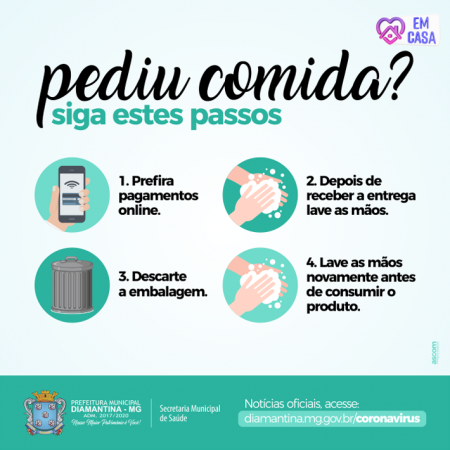
\includegraphics[width=4.68750in,height=4.68750in]{media/image36.png}

Glossário:

\textbf{consumir}: usar.

\textbf{descarte}: jogar no lixo.

PREFEITURA DE DIAMANTINA. Coronavírus -- Covid-19 em Diamantina.
Disponível em:

https://diamantina.mg.gov.br/coronavirus-covid-19-em-diamantina-2/.
Acesso em: 28 fev. 2023.

Com base na leitura do cartaz, as mãos devem ser lavadas

(A) duas vezes após receber a entrega.

(B) depois de usar o produto.

(C) ao descartar a embalagem no lixo.

(D) depois da entrega e antes de usar o produto.

Saeb D6 - Utilizar informações oferecidas por um glossário, verbete de
dicionário ou texto informativo na compreensão ou interpretação do
texto.

BNCC EF15LP03: Localizar informações explícitas em textos.

(A) Incorreta. Embora o cartaz indique que se lave as mãos duas vezes,
nessa ação não ocorre após receber a entrega, mas sim uma vez ao receber
a entrega e outra antes de consumir o produto.

(B) Incorreta. As mãos devem ser lavadas antes de consumir o produto, e
não depois.

(C) Incorreta. No cartaz, não há informações para lavar as mãos ao jogar
descartar a embalagem no lixo.

(D) Correta. Ao ler o cartaz da campanha, identifica-se que ela
incentiva e instrui o leitor a lavar as mãos duas vezes, após a pessoa
receber a entrega e antes de usar o produto.

\textbf{2.}

Leia o início do conto maravilhoso ``Os quatro irmãos espertos''.

\textbf{Os quatro irmãos espertos}

Era uma vez um pobre homem que tinha quatro filhos; muito lhe custou a
educá-los, mas enfim sempre o conseguiu. Quando já estavam crescidos,
disse-lhes:

``Meus ricos filhos, não posso de modo algum continuar a sustentá-los.
Precisam, pois, ir pelo mundo fora e aprender um ofício para que possam
ganhar a vida.''

Depois de lhes ter ainda dado a cada um meio quilo de pão e um bom
cajado, despediram-se do pai e saíram juntos da cidade. {[}\ldots{}{]}

OS QUATRO irmãos espertos. \textbf{Contos dos Irmãos Grimm}. Rio de
Janeiro: Livraria Garnier, 1932, p. 59. Disponível em:
https://digital.bbm.usp.br/handle/bbm/7812. Acesso em: 28 fev. 2023.

\textbf{Glossário}

ofício: trabalho.

A história é narrada

(A) por um dos irmãos da história.

(B) pelos quatro irmãos, personagens da história.

(C) por um narrador-observador.

(D) pelo personagem ``pobre homem''.

Saeb D6 - Utilizar informações oferecidas por um glossário, verbete de
dicionário ou texto informativo na compreensão ou interpretação do
texto.

BNCC EF35LP26: Ler e compreender, com certa autonomia, narrativas
ficcionais que apresentem cenários e personagens, observando os
elementos da estrutura narrativa: enredo, tempo, espaço, personagens,
narrador e a construção do discurso indireto e discurso direto.

(A) Incorreta. Não existe narrador-personagem.

(B) Incorreta. Os irmãos não narram a história.

(C) Correta. A história é apresentada por meio de um
narrador-observador.

(D) Incorreta. O narrador da história é observador.
\end{quote}

\subsubsection{3. }\label{section-92}

\begin{quote}
Os objetivos dos jornais são informar a população. Leia a capa do jornal
a seguir.

https://auniao.pb.gov.br/noticias/primeira-pagina/capa-26-02.2023

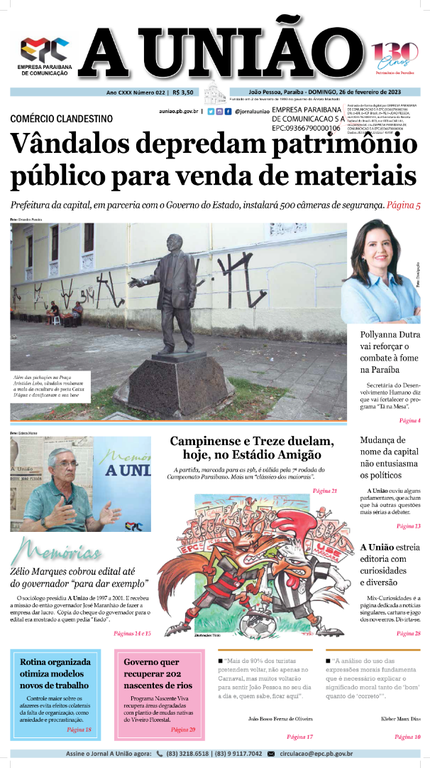
\includegraphics[width=4.47917in,height=8.00000in]{media/image37.png}

A UNIÃO. Capa: 26.02.2023. Disponível em:
https://auniao.pb.gov.br/noticias/primeira-pagina/capa-26-02.2023.
Acesso em: 28 fev. 2023.

O trecho ``Vândalos depredam patrimônio público para venda de
materiais'' é uma

(A) manchete de jornal.

(B) chamada de jornal.

(C) informação sobre esporte.

(D) notícia sobre saúde.

Saeb D3 - Estabelecer relação entre informações num texto ou entre
diferentes textos.

BNCC EF35LP16 - Identificar e reproduzir, em notícias, manchetes, lides
e corpo de notícias simples para público infantil e cartas de reclamação
(revista infantil), digitais ou impressos, a formatação e diagramação
específica de cada um desses gêneros, inclusive em suas versões orais.

(A) Correta. A manchete de uma notícia aparece sempre em negrito e com
letras maiores que o restante do texto.

(B) Incorreta. A chamada está logo após a manchete, em letras menores e
introduz aquilo que foi apresentado na manchete.

(C) Incorreta. A informação contida na manchete não é sobre esporte,
refere-se à \protect\hypertarget{_Hlk128473874}{}{}ação de vândalos que
depredaram patrimônio público para venda de materiais.

(D) Incorreta. Não se trata de uma notícia sobre saúde, e sim sobre a
ação de vândalos que depredaram patrimônio público para venda de
materiais.

\textbf{4.}

Observe as frutas e, com base em seus nomes, responda à questão.

\href{https://www.istockphoto.com/br/foto/ma\%C3\%A7\%C3\%A3-vermelha-com-folha-isolada-no-fundo-branco-gm185262648-19966694?phrase=ma\%C3\%A7\%C3\%A3}{https://www.istockphoto.com/br/foto/ma\%C3\%A7\%C3\%A3-vermelha-com-folha-isolada-no-fundo-branco-gm185262648-19966694?phrase=ma\%C3\%A7\%C3\%A3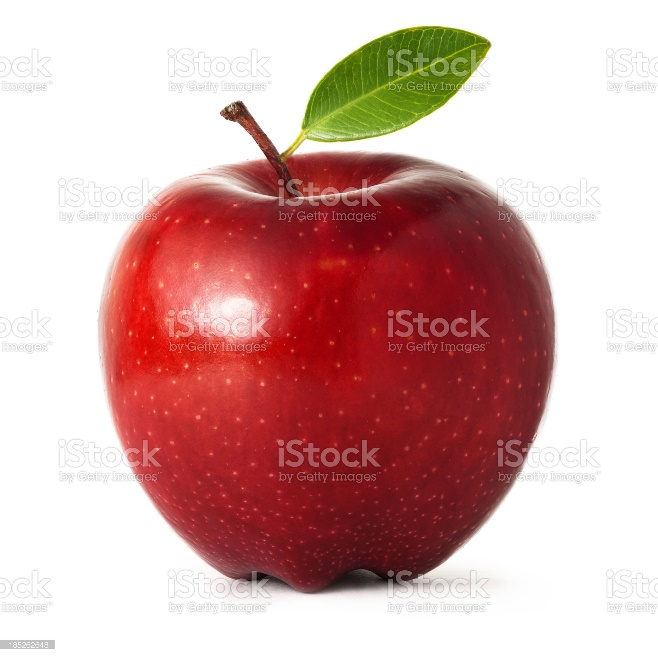
\includegraphics[width=2.98958in,height=2.98958in]{media/image38.jpeg}}

https://www.istockphoto.com/br/foto/mel\%C3\%A3o-honeydew-gm146890371-13998859?phrase=mel\%C3\%A3o

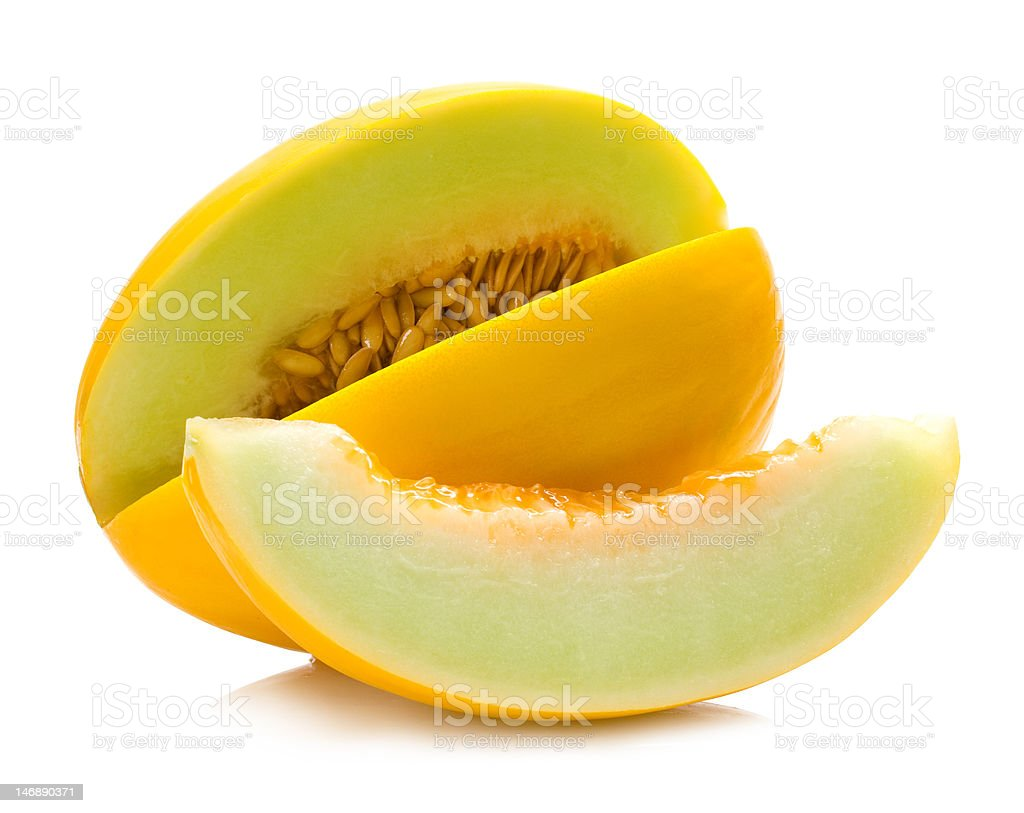
\includegraphics[width=3.33412in,height=2.64722in]{media/image39.jpeg}

https://mail.google.com/mail/u/0/?tab=rm\&ogbl\#search/EF03lp10/FMfcgxwHMGLSpFBBGCZGcQSzrSfLHRQZ?projector=1\&messagePartId=0.1

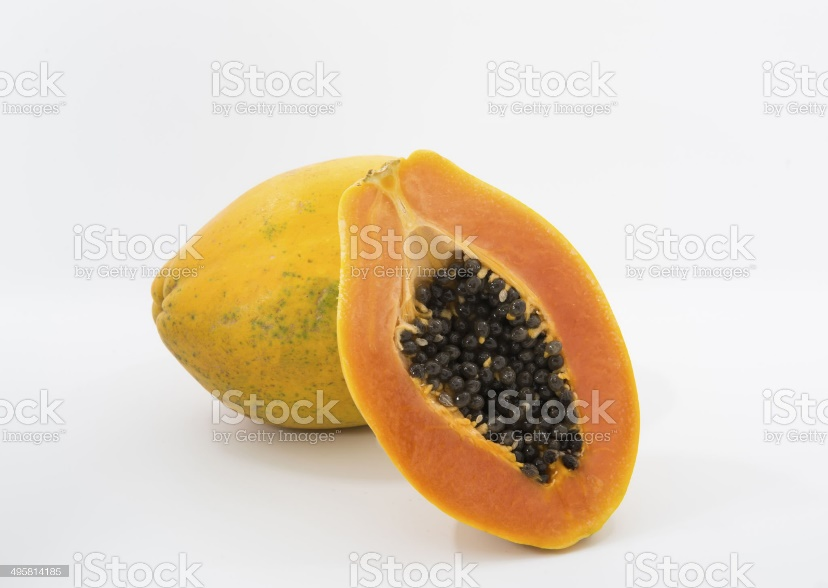
\includegraphics[width=3.76501in,height=2.67500in]{media/image40.jpeg}

A partir da aplicação do sufixo -eiro/-eira nos nomes das frutas, tem-se
o nome das árvores em que esses frutos nascem. Elas são,
respectivamente,

(A) maçãzeira, melãozeiro e mamãozeiro.

(B) maceiro, meleiro, mameiro.

(C) macieira, meloeiro, mamoeiro.

(D) maçãozeira, melãoeiro, mamãoeiro.

Saeb D4 - Identificar o tema central do texto.

BNCC EF03LP10: Reconhecer prefixos e sufixos produtivos na formação de
palavras derivadas de substantivos, de adjetivos e de verbos,
utilizando-os para compreender palavras e para formar novas palavras.

(A) Incorreta. O aluno acrescentou os sufixo -zeiro/-zeira em vez do
sufixo -eiro / -eira.

(B) Incorreta. O aluno retirou incorretamente alguns fonemas para formar
o nome das árvores.

(C) Correta. Maçã, melão e mamão, palavras relativas às imagens, formam:
macieira, meloeiro e mamoeiro.

(D) Incorreta. O aluno apenas acrescentou o sufixo às palavras, sem
entender a regra.
\end{quote}

\section{REFERÊNCIAS}\label{referuxeancias}

\begin{quote}
BRASIL. Ministério da Educação. \textbf{Base nacional comum curricular}:
educação é a base.

BRASIL. Ministério da Educação. \textbf{Pacto nacional pela
alfabetização na idade certa}. Disponível em:
\textless{}http://www.serdigital.com.br/gerenciador/clientes/ceel/material/149.pdf\textgreater{}.
Acesso em: fev. 2023.

KAUFMAN, Ana María; RODRÍGUEZ, María Helena. \textbf{Escola, leitura e
produção de textos}. Porto Alegre: Artmed, 1995.

KOCH, Ingedore G. Villaça. \textbf{Ler e escrever}: estratégias de
produção textual. São Paulo: Contexto, 2010.

LERNER, Delia. \textbf{Ler e escrever na escola}: o real, o possível e o
necessário. Porto Alegre: Artmed, 2002.

NÓBREGA, Maria José. \textbf{Ortografia}. São Paulo: Melhoramentos,
2013.
\end{quote}

\section{SITES}\label{sites}

\begin{quote}
\textbf{Ciência Hoje das Crianças}. Disponível em:
\textless{}http://chc.org.br/\textgreater{}. Acesso em: fev. 2023.

\textbf{DOMÍNIO PÙBLICO}. Disponível em:
\url{http://www.dominiopublico.gov.br/pesquisa/PesquisaObraForm.jsp}.
Acesso em: 28 fev. 2023.

\textbf{RÁDIOS EBC}. Disponível em: https://radios.ebc.com.br/. Acesso
em: 23 fev. 2023.

\textbf{PORTAL Teatro na escola}. Disponível em:
\url{https://www.teatronaescola.com/}. Acesso em: 28 fev. 2023.
\end{quote}
